

%%%%%%%%%%%%%%%%%%%%%%%%%%%%%%%%%%%%%%%%%
% The Legrand Orange Book
% LaTeX Template
% Version 2.4 (26/09/2018)
%
% This template was downloaded from:
% http://www.LaTeXTemplates.com
%
% Original author:
% Mathias Legrand (legrand.mathias@gmail.com) with modifications by:
% Vel (vel@latextemplates.com)
%
% License:
% CC BY-NC-SA 3.0 (http://creativecommons.org/licenses/by-nc-sa/3.0/)
%
% Compiling this template:
% This template uses biber for its bibliography and makeindex for its index.
% When you first open the template, compile it from the command line with the 
% commands below to make sure your LaTeX distribution is configured correctly:
%
% 1) pdflatex main
% 2) makeindex main.idx -s StyleInd.ist
% 3) biber main
% 4) pdflatex main x 2
%
% After this, when you wish to update the bibliography/index use the appropriate
% command above and make sure to compile with pdflatex several times 
% afterwards to propagate your changes to the document.
%
% This template also uses a number of packages which may need to be
% updated to the newest versions for the template to compile. It is strongly
% recommended you update your LaTeX distribution if you have any
% compilation errors.
%
% Important note:
% Chapter heading images should have a 2:1 width:height ratio,
% e.g. 920px width and 460px height.
%
%%%%%%%%%%%%%%%%%%%%%%%%%%%%%%%%%%%%%%%%%

%----------------------------------------------------------------------------------------
%	PACKAGES AND OTHER DOCUMENT CONFIGURATIONS
%----------------------------------------------------------------------------------------

\documentclass[11pt,fleqn]{book} % Default font size and left-justified equations





\usepackage[dvipsnames]{xcolor}






\input{WaterTreatment structure.tex} % Insert the commands.tex file which contains the majority of the structure behind the template

%\hypersetup{pdftitle={Title},pdfauthor={Author}} % Uncomment and fill out to include PDF metadata for the author and title of the book

%----------------------------------------------------------------------------------------

\begin{document}

%----------------------------------------------------------------------------------------
%	TITLE PAGE
%----------------------------------------------------------------------------------------

\begingroup
\thispagestyle{empty} % Suppress headers and footers on the title page
%\begin{center}
%
\includegraphics[scale=0.6]{Blank.png}\\
%
\includegraphics[scale=0.6]{SCC_Logo_Primary.png}
%\end{center}
\newpagecolor{BurntOrange}\afterpage{\restorepagecolor}
\begin{tikzpicture}[remember picture,overlay]
%\node[inner sep=0pt] (background) at (current page.center) {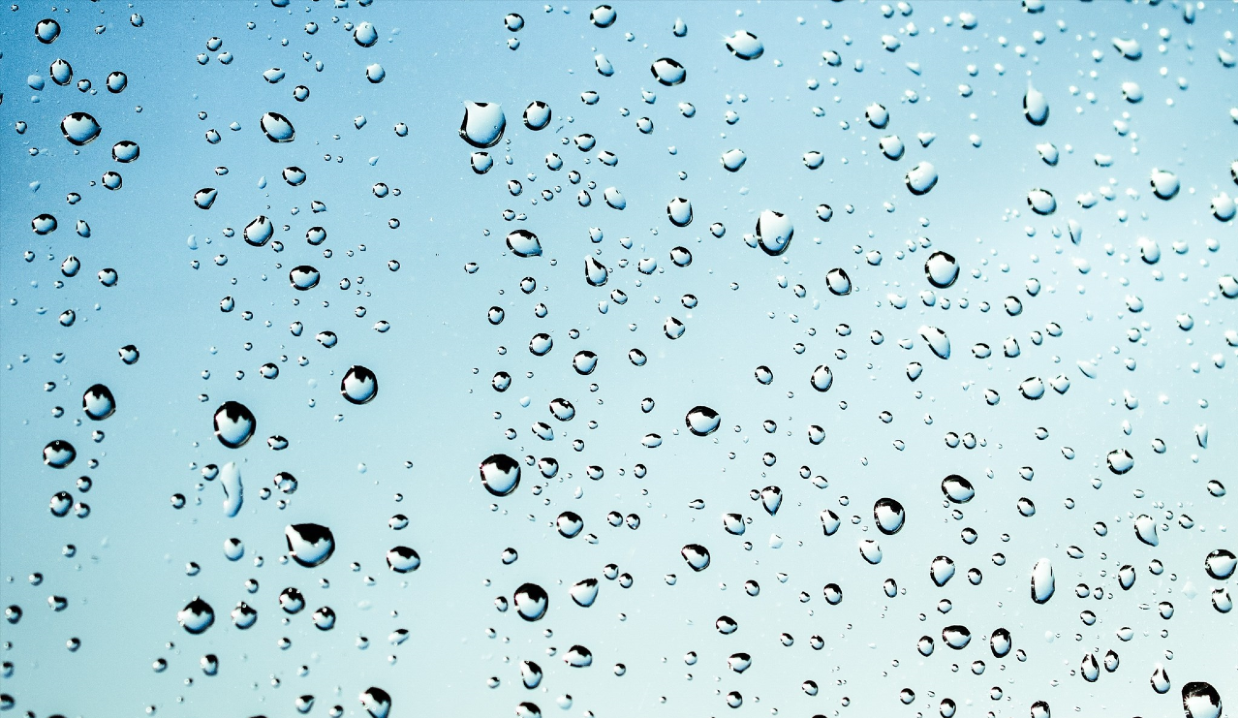
\includegraphics[width=\paperwidth]{Water3.png}};

\node[inner sep=0pt] (background) at (current page.center) {\includegraphics[width=\paperwidth]{WaterBackground1.png}};


\draw (current page.center)node [fill=blue!1!white!10,fill opacity=.3,text opacity=1,inner sep=2cm] { \Huge\centering\bfseries\sffamily\parbox[c][][t]{\paperwidth}{\centering \textcolor{Bittersweet}{} \\\textcolor{BurntOrange}{Water Treatment}\\[15pt] % Book title
% {\Large A Profound Subtitle}\\[20pt] % Subtitle
{\large Shabbir Basrai}}}; % Author name
\end{tikzpicture}
\begin{center}

\includegraphics[scale=1]{BassettCTCLogo.png}
\end{center}
\vfill
\endgroup

%----------------------------------------------------------------------------------------
%	COPYRIGHT PAGE
%----------------------------------------------------------------------------------------

\newpage
~\vfill
\thispagestyle{empty}

\noindent Copyright \copyright\ 2022 Shabbir Basrai\\ % Copyright notice
%
%\noindent \textsc{Published by Publisher}\\ % Publisher
%
%\noindent \textsc{book-website.com}\\ % URL
%
%\noindent Licensed under the Creative Commons Attribution-NonCommercial 3.0 Unported License (the ``License''). You may not use this file except in compliance with the License. You may obtain a copy of the License at \url{http://creativecommons.org/licenses/by-nc/3.0}. Unless required by applicable law or agreed to in writing, software distributed under the License is distributed on an \textsc{``as is'' basis, without warranties or conditions of any kind}, either express or implied. See the License for the specific language governing permissions and limitations under the License.\\ % License information, replace this with your own license (if any)

\noindent \textit{Revision Date: August, 2022} % Printing/edition date

%----------------------------------------------------------------------------------------
%	TABLE OF CONTENTS
%----------------------------------------------------------------------------------------

%\usechapterimagefalse % If you don't want to include a chapter image, use this to toggle images off - it can be enabled later with \usechapterimagetrue

\chapterimage{Preliminary.jpg} % Table of contents heading image

\pagestyle{empty} % Disable headers and footers for the following pages

\tableofcontents % Print the table of contents itself

\cleardoublepage % Forces the first chapter to start on an odd page so it's on the right side of the book

\pagestyle{fancy} % Enable headers and footers again

%----------------------------------------------------------------------------------------
%	PART
%----------------------------------------------------------------------------------------

\part{Week 1}
%\documentclass{article}
%%\usepackage[english]{babel}%
%\usepackage{graphicx}
%\usepackage{tabulary}
%\usepackage{tabularx}
%\usepackage[table,xcdraw]{xcolor}
%\usepackage{pdflscape}
%\usepackage{lastpage}
%\usepackage{multirow}
%\usepackage{afterpage}
%\usepackage{rotating}
%\usepackage{pdfpages}
%\usepackage{cancel}
%\usepackage{amsmath}
%\usepackage[table]{xcolor}
%\usepackage{caption}
%\captionsetup{font=scriptsize,labelfont=scriptsize}
%\usepackage{pdflscape}
%\usepackage{fixltx2e}
%\usepackage[T1]{fontenc}
%\usepackage[utf8]{inputenc}
%\usepackage{multirow}
%\usepackage{ifthen}
%\usepackage{fancyhdr}
%\usepackage[document]{ragged2e}
%\usepackage[margin=1in,top=1.2in,headheight=57pt,headsep=0.1in]
%{geometry}
%\usepackage{ifthen}
%\usepackage{fancyhdr}
%\everymath{\displaystyle}
%\usepackage[document]{ragged2e}
%\usepackage{fancyhdr}
%\usepackage[table,xcdraw]{xcolor}
%% If you use beamer only pass "xcolor=table" option, i.e. \documentclass[xcolor=table]{beamer}
%\usepackage[normalem]{ulem}
%\useunder{\uline}{\ul}{}
%\everymath{\displaystyle}
%\linespread{2}%controls the spacing between lines. Bigger fractions means crowded lines%
%%\pagestyle{fancy}
%%\usepackage[margin=1 in, top=1in, includefoot]{geometry}
%%\everymath{\displaystyle}
%\linespread{1.3}%controls the spacing between lines. Bigger fractions means crowded lines%
%%\pagestyle{fancy}
%\pagestyle{fancy}
%\setlength{\headheight}{56.2pt}
%
%
%\chead{\ifthenelse{\value{page}=1}{
\includegraphics[scale=0.3]{BassettCTCLogo}\\ \textbf \textbf Water - General Introduction}}
%\rhead{\ifthenelse{\value{page}=1}{Shabbir Basrai}{Shabbir Basrai}}
%\lhead{\ifthenelse{\value{page}=1}{}{\textbf Water - General Introduction}}
%
%
%\cfoot{}
%\lfoot{Page \thepage\ of \pageref{LastPage}}
%\rfoot{}
%\renewcommand{\headrulewidth}{2pt}
%\renewcommand{\footrulewidth}{1pt}
%\newcommand{\comment}[1]{\hspace{0em}{\small\textit{#1}}\bigskip\par}
%\begin{document}


\chapterimage{WaterChapterImage1}
\chapter{Water - General Introduction}

\vspace{0.2cm}
\begin{center}
\textbf{\textit{“If there is magic on this planet, it is contained in water.”}}
\end{center}
\begin{flushright}
\textit{Loren Eiseley}
\end{flushright}
\vspace{0.2cm}


\section{Regulations}\index{Regulations}
\begin{itemize}
\item USEPA administers the nationwide drinking water program as authorized under the 1974 federal SDWA, which was substantially amended in 1986 and 1996. The federal program consists of the establishment of drinking water standards, monitoring and reporting requirements, and public notification, which are applicable to all public water systems.
USEPA can directly enforce compliance of these standards, or authorize primary enforcement of the federal SDWA to any state that has an authorizing state statute at least as stringent as the federal SDWA, and a state regulatory program for public water systems that meets various enforcement, planning, and record keeping requirements.
Authorization of primary enforcement of the federal SDWA to a state is known as "primacy." As part of the delegation of primacy to a state, USEPA provides oversight and partial grant funding of the state program as well as annual capitalization grants under the Drinking Water State Revolving Fund (DWSRF). The oversight by USEPA requires an annual work plan, an annual (DWSRF) Intended Use Plan, and specific reporting requirements including an annual PWS compliance report.
\item The federal Safe Drinking Water Act (SDWA) establishes the foundation and standards for each state to be the primacy agency for the enforcement of the SDWA for public water systems (PWS) within their boundaries. California has carried out the drinking water program as the primacy agency since the inception of the federal SDWA. The fundamental requirement for primacy is that California adopt and implement standards that are at least as stringent as the federal drinking water standards. Under primacy, each state is free to adopt standards that are more stringent than those adopted at the federal level.
The regulation of drinking water in California has developed over the last 45 years under the SDWA. 
\item A major milestone in this development was the transfer of the Drinking Water Program to the State Water Board in 2014. Since that transfer, many facets of the drinking water program within the State Water Board have been bolstered by the growing coordination and assistance of other divisions and programs within the State Water Board. \item Although the State Water Board has the fundamental responsibility for the regulatory oversight of drinking water, other agencies play important roles. Because of the importance of drinking water, there has been an increased focus on coordination and communication of the roles and responsibilities.
State Agencies
\item The regulation of water supply, water quality, and the various types of water systems that serve drinking water is shared among several agencies, including local agencies, in California. However, California took a major step forward in integrating the regulation of water quality when it transferred the state’s Drinking Water Program from the California Department of Public Health (CDPH) to the State Water Board on July 1, 2014. One of the Administration’s goals in transferring the program was to promote safe drinking water through more integrated water quality management, from source to tap.
Most of the statutory authority for regulation of drinking water is in the California Health and Safety (H\&S) Code. Under the H\&S Code, the State Water Board has primary responsibility for regulating all public water systems. There are three other state agencies that also regulate certain aspects of specific classes of systems including:
The California Public Utilities Commission (CPUC) for investor-owned systems
The Division of Corporations (DOC) for mutual water companies
The Department of Housing and Community Development (DHCD) for mobile home parks.
Additionally, the Department of Water Resources (DWR), the Office of Environmental Health Hazard Assessment (OEHHA), the Secretary of State, and the Department of Real Estate are also involved in activities impacting public water systems.
\item The State Water Board carries out the responsibilities as the federally designated primacy agency for the drinking water program in California. This includes responsibility for the implementation of the federal Safe Drinking Water Act (SDWA). Additionally, the State Water Board carries out the responsibility for implementation of the California SDWA. These responsibilities are set forth in Chapter 4 of Part 12 (Drinking Water) of Division 104 (Environmental Health) of California H\&S Code (Section116270 et seq.) and Articles 1 and 2 of Group 4, of Subchapter 1 of Chapter 5 (Sanitation) of Division 1 (Department of Health Services) of Title 17 and Chapters 1 through 19 of Division 4 (Environmental Health) of Title 22 of the California Code of Regulations (CCR). The DDW within the State Water Board carries out the drinking water regulatory responsibilities.
DDW implements the Safe Drinking Water Act and California regulations applicable to public water systems. This direct implementation of the program is carried out at the local and regional level by DDW District Offices and Local Primacy Agencies. The overall management, support and control of the program is accomplished through the larger management structure, ultimately under the State Water Board members. The program includes a broad range of elements and functions discussed further below.
DDW includes the Environmental Laboratory Accreditation Program (ELAP) which is responsible for accreditation of laboratories that analyze environmental samples for regulatory purposes, including drinking water laboratories performing analyses pursuant to the California SDWA. The ELAP program is of critical importance to a range of programs other than drinking water within the State Water Board and other partner agencies.
DDW is also responsible for adopting uniform criteria for the use of recycled water that is protective of public health. The Regional Water Boards or the Division of Water Quality (DWQ) within the State Water Board incorporate DDW-developed criteria in Water Reclamation Permits or Waste Discharge Requirements, which set out the specific requirements that a water recycling project must meet.
DDW and the Regional Water Boards/DWQ work cooperatively on regulating water recycling projects including those that are designed to augment drinking water supplies, including recharging groundwater supplies and augmenting surface water supplies such as reservoirs, as well as implementing statutory requirements with the goal of developing standards for the safe use of recycled water for direct potable reuse.
To better demonstrate the work performed by DDW, program metrics on completed sanitary surveys and permits are reported by the State Water Board annually as part of the annual performance report available to view on the State Water Board website. The most recent annual performance report is for the Fiscal Year 2018-19 posted here: 
\item DWQ and the Regional Water Boards are responsible for protecting the quality of surface and groundwater (namely lakes, rivers, and groundwater basins) for all beneficial uses including municipal and domestic supply. DWQ and the Regional Water Boards adopt statewide and regional water quality control plans that establish beneficial uses of surface and groundwaters, water quality objectives for a variety of constituents to protect those uses, and a program of implementation to achieve the water quality objectives. The program of implementation typically includes monitoring and surveillance, permitting, and enforcement. DWQ and the Regional Water Boards have the authority to issue waste discharge permits to the following:
\begin{itemize}
\item any entity that discharges wastes to surface or groundwaters including municipal or
\item industrial wastewater treatment plants
\item municipalities or facilities that discharge stormwater
\item agricultural operations
\item food processing facilities
\item mining facilities
\item timber harvest operations
\end{itemize}
As a part of these permitting programs, DWQ and the Regional Water Boards also issue orders to clean up and abate spills and leaks.
DWQ administers the state’s GAMA program, which collects data from private wells and groundwater basins and makes it available through the GeoTracker GAMA online data system. The GAMA program coordinates and shares monitoring data with DDW to avoid duplication of effort and increase the amount of data that DDW can use to advise water systems about the underlying groundwater quality.
DWQ establishes statewide policies for water quality control such as the Recycled Water Policy. The Recycled Water Policy establishes monitoring requirements for water recycling facilities including those that propose to produce recycled water for indirect potable reuse.
\item The CPUC is responsible for ensuring that California’s investor-owned water utilities deliver clean, safe, and reliable water to their customers at reasonable rates. As of November 2020, the CPUC Water Division regulates 93 investor-owned water and 12 sewer utilities under the CPUC’s jurisdiction providing water service to about 16 percent of California’s residents. Approximately 98 percent of is the customers are served by 9 large water utilities each serving more than 10,000 connections. Annual water and wastewater revenues under the CPUC’s regulation total \$1.96 billion.
The CPUC's five commissioners are appointed by the Governor and confirmed by the state Senate. The CPUC's primary source of funding is from a "user fee" that is assessed on utility customers as a percentage of each regulated utility’s gross in-state operating revenues.
The CPUC ensures that customers of regulated water utilities receive safe and reliable water service while allowing the utility to earn a reasonable return on its investment. Its functions include: (1) authorizing utility service within defined service areas, (2) setting rates, and (3) regulating the quality of service.
As a result of shared responsibility for the regulation of investor-owned utilities with respect to water quality, the CPUC and the State Water Board’s DDW have maintained a formal memorandum of understanding (MOU) to ensure consistency and coordination between the agencies’ two programs. This memorandum defines common objectives, principles, agency responsibilities, and project coordination. The staff of the two agencies routinely meet to ensure that the goals of the MOU are being complied with, and to coordinate the
\item activities between the two agencies. The large (Class A) investor-owned utilities have acknowledged the coordination between the two organizations and may participate in joint meetings with the staff of both agencies. The CPUC can impose stricter water quality requirements; an example being the CPUC requirement that Class A utilities implement the distribution system operations plan of the California Water Works Standards, which is a more stringent requirement than that which DDW mandates.
Issues related to the small investor-owned utilities continue to be difficult to resolve because these systems may lack the Technical, Managerial and Financial (TMF) capacity to secure rate relief and have an insufficient number of customers to properly fund infrastructure improvements. There has been some success in reducing the number of CPUC-jurisdictional water utilities by one-third over the last twenty years. Many of the  small investor-owned utilities experience significant infrastructure problems, such as leaking water pipes, undersized water storage facilities, inadequate fire service, and their revenue from water sales being insufficient to address these problems. In addition, present state infrastructure funding opportunities are underutilized by investor owned utilizes given the taxability of grants under the Tax Cuts and Jobs Act of 2017. Thus, the small companies are limited to seeking loans, for which they may have difficulty meeting the TMF capacity requirements, which would demonstrate their capability of managing the infrastructure project and paying back the loan.
In 2012, the Legislature passed Chapter 539, Statutes of 2012 (AB 1830), amending Public Utilities Code Section 2705.6 which allowed complaints to be filed by tenants of mobile home parks claiming that their water rates were not just and reasonable or that the service was inadequate. The CPUC reported to State Water Board staff that the Commission has received two Section 2705.6 complaints as of September 2019.
\item the United States Environmental Protection Agency (USEPA)is responsible for implementing federal drinking water law, setting national drinking water requirements.

\item The regulation of the state’s drinking water is primarily the responsibility of the State Water Board. 

\item Along with the regulation of drinking water, the State Water Board and the Regional Water Quality Control Boards (Regional Water Boards), (collectively the “Water Boards”) are responsible for protecting the waters of the state.

\item the Office of Environmental Health Hazard Assessment (OEHHA) is responsible for providing the State Water Board with health- based risk assessments for contaminants, which are used to develop primary drinking water standards that protect public health.

\item the California Public Utilities Commission (CPUC) shares regulatory responsibility for ensuring the quality of water supplied by investor-owned water utilities subject to its jurisdiction and is responsible for overseeing their rate structures.


\item Local agencies also have a role in drinking water regulation through direct oversight of certain PWS and through activities that affect a PWS service area.


\item Local Agency Formation Commissions (LAFCO) oversee the expansion of service areas of public agencies that are PWS and can review them to determine if an agency is operating acceptably including the delivery of safe drinking water.

However, the regulation of water supply, water quality, and the types of water systems that serve drinking water remains divided in California. There are several agencies within the state that have a role in regulating PWS, including formation, design, construction, operations, and the rates they can charge customers.
 This includes drinking water sources, both surface water and groundwater supplies. Other state agencies are involved too. For example,  As another example, 
, and overseeing the State Water Board’s exercise of primary

\begin{figure}
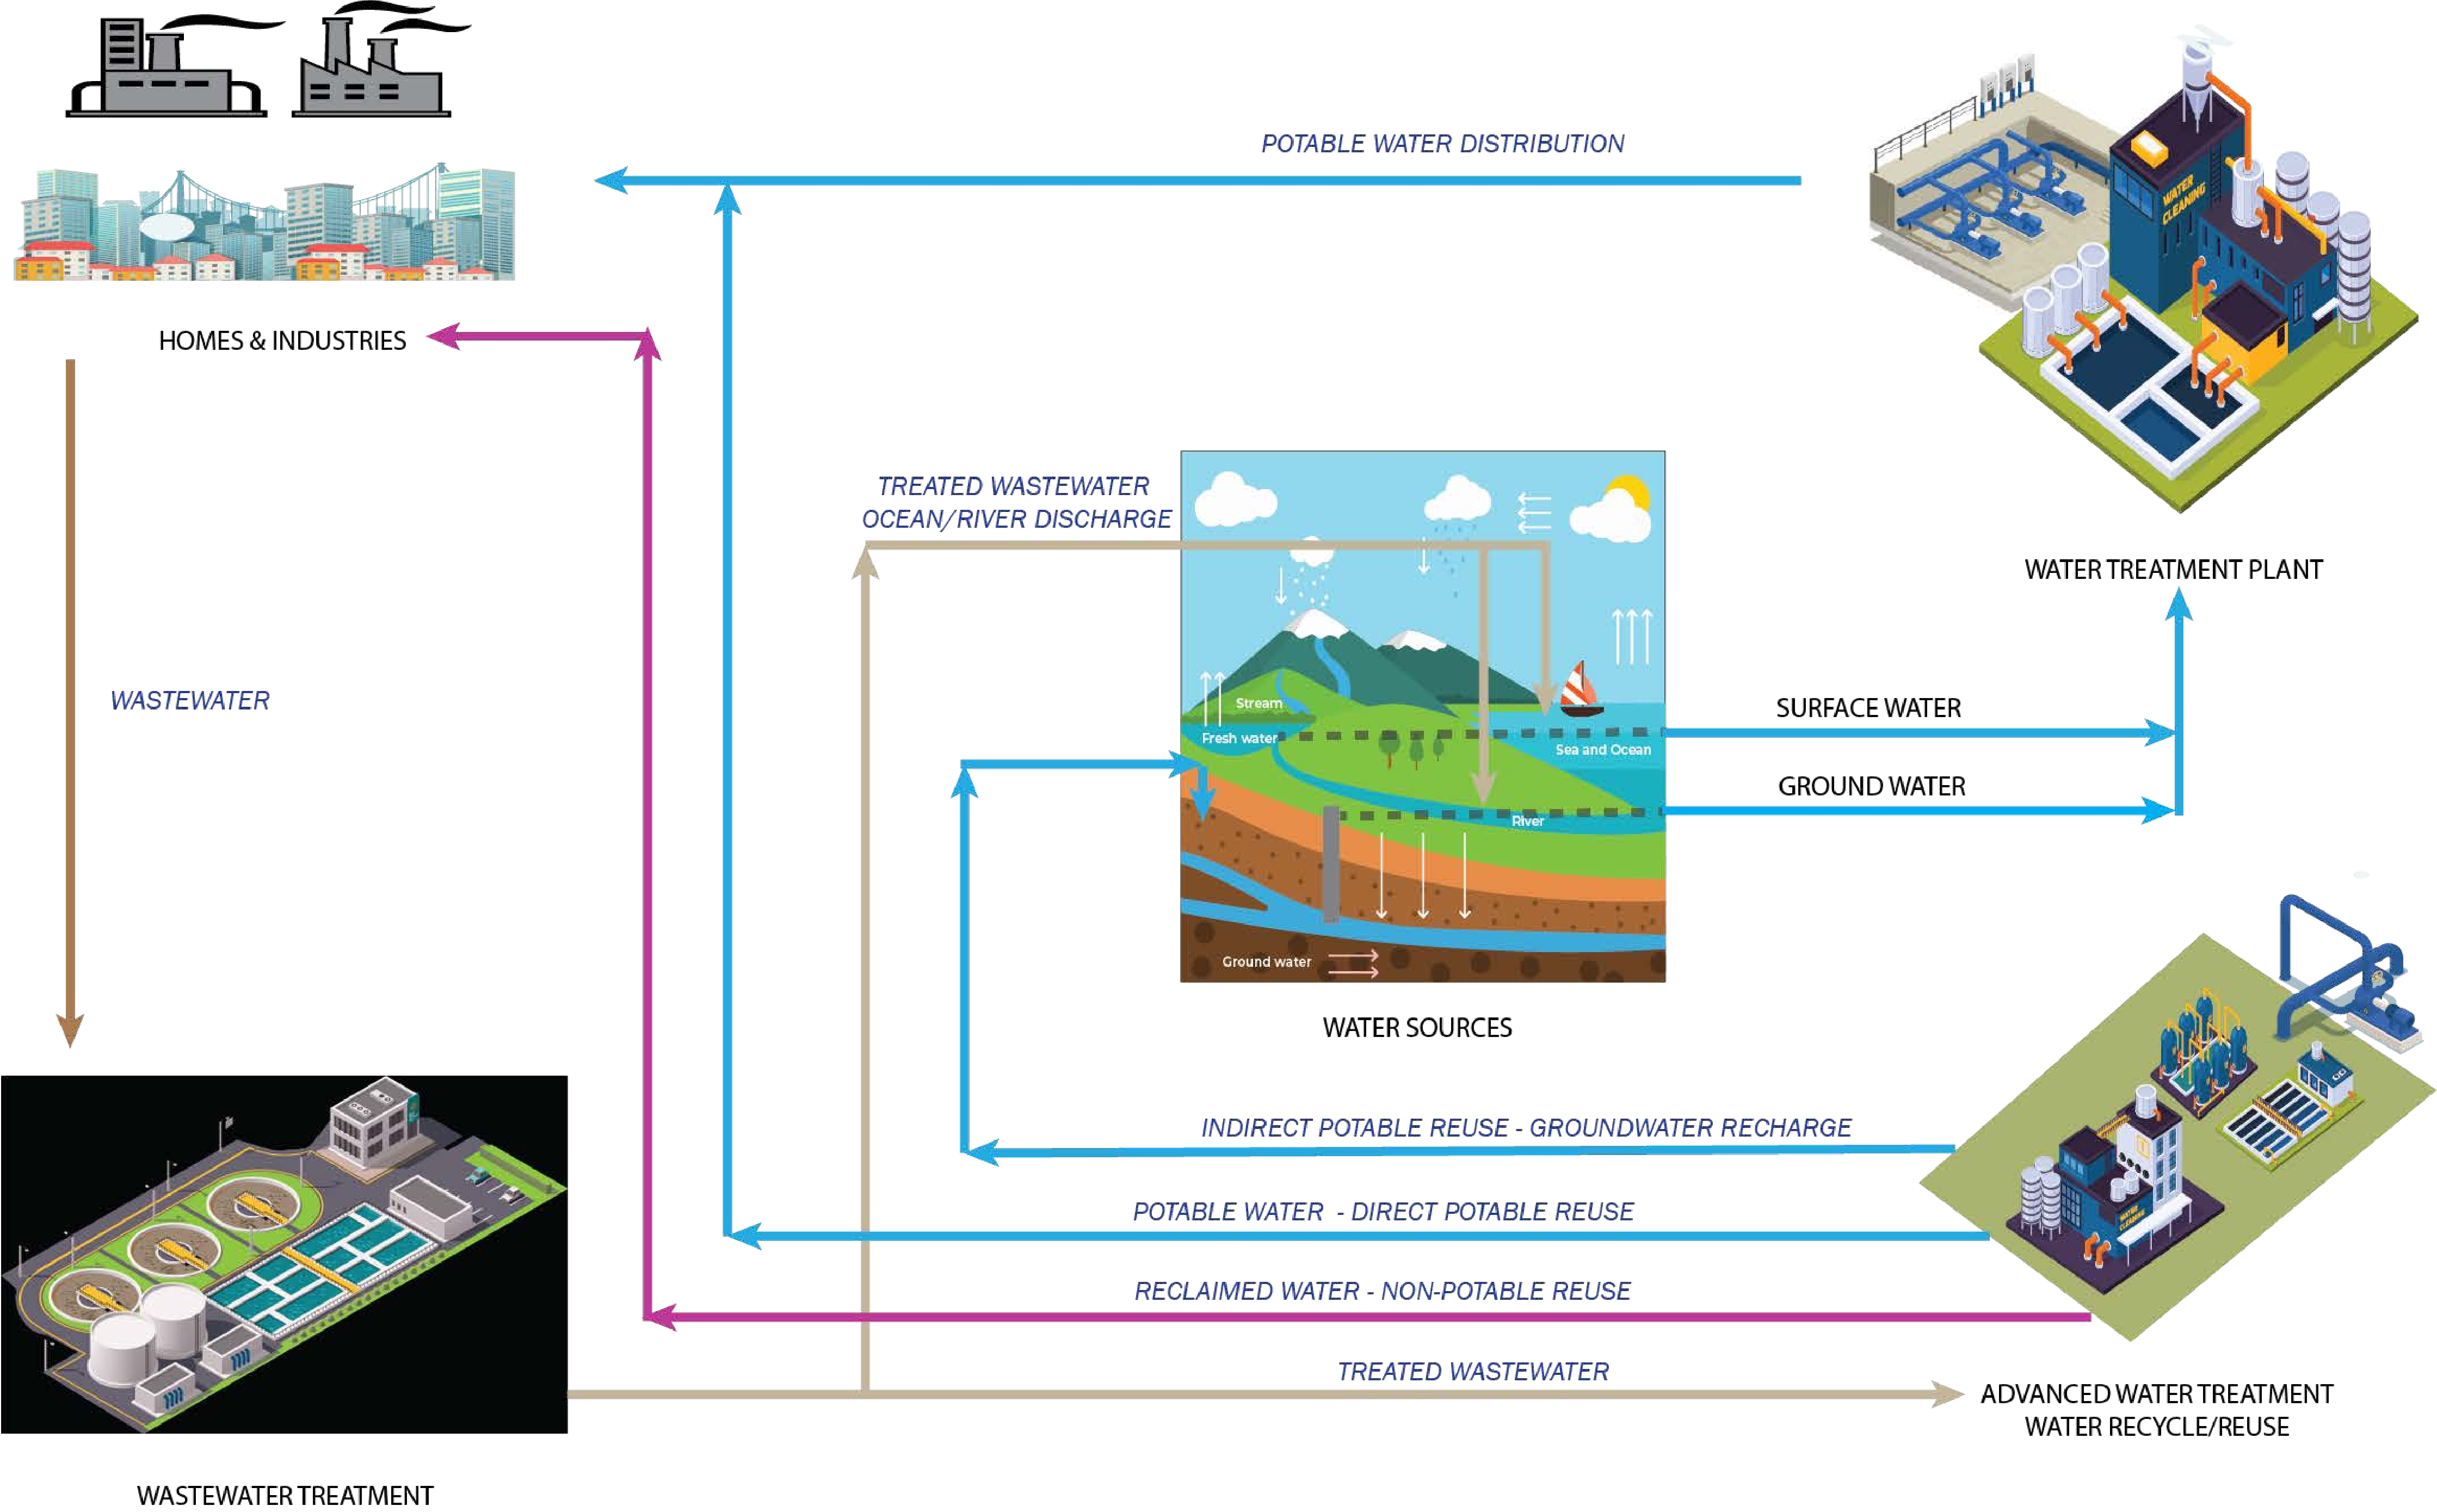
\includegraphics[scale=0.2]{Test4}\\
\captionof{figure}{TypesofPWS1}%\caption{}
\end{figure}


\item In 1989, the California Legislature enacted Assembly Bill (AB) 21 (Chapter 823, Statutes of 1989) which directed the California Department of Health Services (CDHS) to undertake a comprehensive assessment of drinking water in California: its quality and safety, types of problems, overall health risks, current and projected costs, and current regulatory programs. From this assessment, CDHS was directed to develop a plan, containing specific recommendations, to resolve any problems and improve the overall quality and safety of California's drinking water.
\item In 2012, California became the first state to enact a Human Right to Water statute (Chapter 524, Statutes of 2012 (AB 685, Eng)) declaring that it is “the established policy of the state that every human being has the right to safe, clean, affordable, and accessible water adequate for human consumption, cooking, and sanitary purposes.”
\item The Sustainable Groundwater Management Act (SGMA) became law in 2014 based on a three-bill legislative package, composed of AB 1739 (Dickinson), SB 1168 (Pavley), and SB 1319 (Pavley). As a result, for the first time California has a framework for sustainable, groundwater management. As stated in the statutes, this means that many basins are now required to undertake “management and use of groundwater in a manner that can be maintained during the planning and implementation horizon without causing undesirable results.”



\item Any water system serving 15 residences or an average of at least 25 people more than 60 days out of the year is a public water system. A source of confusion is the term “public water system” that is established in federal law and is used in California as well. The handout titled “What is a Public Water System” provides additional clarification. “Public” water systems serve the public but can be either publicly-owned or privately-owned.  Public water systems can be broken down into community and non-community systems and non-community systems can either be transient or non-transient, resulting in three types of water systems (community, transient non-community and non-transient non- community).

\item There are approximately 7,369 PWS
\item Approximately eight percent serve large communities with more than 10,000 service
\item Many of the small PWS are challenged by lack of technical, managerial, and financial (TMF) capacity and do not provide water that meets drinking water standards.
\item 63 percent serve small communities with fewer than 200 service connections (corresponding to fewer than 660 people)
\item More than 100 voluntary physical and managerial consolidations and water partnerships have occurred since 2017. Most of the consolidations addressed bacteriological contamination (coliform), chemical contaminants (arsenic, nitrate, volatile organic compounds, and disinfection byproducts), or radiological contamination (uranium). Some consolidations addressed water outages and reliability issues associated with a single source of supply, while other consolidations addressed lead and copper violations, lack of TMF capacity, and systems destroyed by wildfire.
\item Benefits are: increased reliability and sustainability of system, increased customer base and ability to afford system upgrades
\item the State Water Board also initiated 17 mandatory consolidations of small systems serving disadvantaged communities.

\item Small water systems have several barriers to funding their operations. As mentioned above, they often lack managerial and financial capacity because they may not have the experience or skill set to run a
\item public water system properly. Their customer base may be too small to generate enough revenue to meet their operational costs or to qualify for wholesale pricing of materials that may be available to larger systems. They often appear reluctant to raise the water rates of their customers to cover the costs of operations and maintenance and may delay system repair and replacement activities because of inadequate funding.
In addition, water system customers in small communities, particularly economically disadvantaged ones, may have difficulties paying their water bills, regardless of whether the rates are high enough to support an adequately run system. When customers cannot pay and are cut off from service, this further contributes to inadequate funding for the small water system.
\item Over the past decades, the cost of drinking water, adjusted for inflation, has been on the rise and this trend is expected to continue. To address the issue of affordability, there is a need for a statewide rate assistance program
\end{itemize}
enforcement responsibility, which means that the State Water Board has the main responsibility for enforcing drinking water regulations.
 The State Water Board may opt to allow 
Mirroring the regulatory scope of the State Water Board, the scope of this Plan focuses on the state’s PWS, as defined in Health and Safety Code 116275(h). These are systems that either have (a) 15 or more service connections or (b) systems that serve at least 25 individuals daily at least 60 days out of
the year. There were 7,369 PWS in the state as of November 2020. This is a significant decrease from the more than 10,000 systems that existed in 1993. Additionally, California’s population has grown from approximately 29 million at that time to over 40 million.
Figure 1 shows the breakdown  connections (corresponding to approximately 33,000 people). The number of large community water systems is surpassed by the number of small community water systems.
Of the current number of community water systems, .


%\section{Water Parameters}\index{Water Parameters}
%\section{Physical}\index{Physical}
%\section{Chemical}\index{Chemical}
%\section{Contaminants}\index{Contaminants}
%\section{Monitoring and Sampling}\index{Monitoring and Sampling}
%\section{Laboratory and Field Analysis}\index{Laboratory and Field Analysis}
%\section{Water Treatment}\index{Water Treatment}
%\section{Screening}\index{Screening}
%\section{Coagulation}\index{Coagulation}
%\section{Flocculation}\index{Flocculation}
%\section{Sedimentation}\index{Sedimentation}
%\section{Filtration}\index{Filtration}
%\section{Hardness Treatment}\index{Hardness Treatment}
%\section{Fluoridation}\index{Fluoridation}
%\section{Organic Removal}\index{Organic Removal}
%\section{Inorganic Removal}\index{Inorganic Removal}
%
%\section{Water introduction}\index{Water introduction}
%\subsection{Water properties}\index{Water properties}

\begin{minipage}{.7\textwidth} 
\begin{itemize}
\item Its chemical formula, H$_2$O, indicates that each of its molecules contains one oxygen and two hydrogen atoms, connected by covalent bonds. The hydrogen atoms are attached to the oxygen atom at an angle of 104.45\si{\degree}
\end{itemize}.
    \end{minipage}%
        \begin{minipage}{0.3\textwidth}
        \centering
        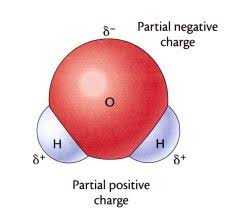
\includegraphics[scale=0.4]{Waterpolarity}
    \end{minipage}\\
\vspace{0.5cm}
\begin{itemize}
\item Unique properties of water arise from the shape of its molecule which is comprised of a much larger oxygen atom and two smaller hydrogen atoms.  Even though the water molecule is overall neutral, its bent shape results in the accumulation of positive charge near the oxygen end and negative charge near the hydrogen.  This differential in charges makes the water molecule polar. 

\item The constituents, size and polarity of the water molecule imparts unique properties which makes water vital not only for the existence of all biological lifeforms and for other non-biological aspects critical for the survival and progress of the human race.

\item Water makes up 60-75\% of human body weight. A loss of just 4\% of total body water leads to dehydration, and a loss of 15\% can be fatal. A person could survive a month without food but wouldn’t survive 3 days without water.\\
\end{itemize}

\subsection{Water use}\index{Water use}
\begin{itemize}
\item Besides it being needed for basic sustenance of all living beings, water is vital element for the world economy and sustenance of the human society in various ways including:
\begin{itemize}
\item As a food source - fishing
\item For commerce - shipping, trade and transportation
\item For recreation - swimming, skiing, surfing etc.
\end{itemize}
\item Breakdown of global freshwater use:\\
70\% is used for agriculture\\
19\% is used by industries, and \\
11\% is for municipal use

\item In the USA, average water consumption per person is about 80-100 gallons per day.

\end{itemize}

\section{Water Supplies}\index{Water Supplies}
\begin{itemize}
\item The water on our Earth today is the same water that has been here for nearly 5 billion years.\\
\item Water molecules were formed in interstellar space by chemical reactions between hydrogen molecules and oxygen-bearing molecules such as carbon monoxide and the Earth inherited its water from asteroids and comets crashing into it.
\item The only thing that changes is the form that water takes as it travels through the water cycle.
\item On Earth, water is the only substance that can occur naturally in its three states of matter -  gas, liquid and solids, circulates naturally through its five principal realms:
\begin{itemize}
\item Oceans
\item Atmosphere
\item Lakes and rivers
\item Icecaps and glaciers
\item Underground
\end{itemize}
This is the planetary Water Cycle.
\item Life on earth is dependent on the Earth's water cycle
\item Civilizations have always formed near water sources - on the banks of rivers. Ancient Egyptians - on the Nile, Mesopotamians in the Fertile Crescent on the Tigris/Euphrates rivers, Ancient Chinese on the Yellow River, and the Ancient India on the Indus.
\newpage
\begin{figure}[]
\begin{center}
\includegraphics[scale=0.8]{Watercycle1}
\caption{Water Cycle}
\textit{(Credit:David Cain/NWS)}
\end{center}
\end{figure}
\item Water covers about 71\% of Earth's surface.  The distribution of Earth's water is provided in the below table.

% Please add the following required packages to your document preamble:
% \usepackage{multirow}
\begin{table}[ht]
\begin{center}
\begin{tabular}{|l|l|llll}
\hline
\multirow{9}{*}{Fresh water} & \multirow{9}{*}{2.50\%} & \multicolumn{1}{l|}{\multirow{7}{*}{Surface water}} & \multicolumn{1}{l|}{\multirow{7}{*}{1.20\%}} & \multicolumn{1}{l|}{Atmosphere}                & \multicolumn{1}{l|}{3.00\%}  \\ \cline{5-6} 
                             &                         & \multicolumn{1}{l|}{}                               & \multicolumn{1}{l|}{}                        & \multicolumn{1}{l|}{Living things}             & \multicolumn{1}{l|}{0.26\%}  \\ \cline{5-6} 
                             &                         & \multicolumn{1}{l|}{}                               & \multicolumn{1}{l|}{}                        & \multicolumn{1}{l|}{Rivers}                    & \multicolumn{1}{l|}{0.49\%}  \\ \cline{5-6} 
                             &                         & \multicolumn{1}{l|}{}                               & \multicolumn{1}{l|}{}                        & \multicolumn{1}{l|}{Swamps, marshes}           & \multicolumn{1}{l|}{2.60\%}  \\ \cline{5-6} 
                             &                         & \multicolumn{1}{l|}{}                               & \multicolumn{1}{l|}{}                        & \multicolumn{1}{l|}{Soil moisture}             & \multicolumn{1}{l|}{3.80\%}  \\ \cline{5-6} 
                             &                         & \multicolumn{1}{l|}{}                               & \multicolumn{1}{l|}{}                        & \multicolumn{1}{l|}{Lakes}                     & \multicolumn{1}{l|}{20.90\%} \\ \cline{5-6} 
                             &                         & \multicolumn{1}{l|}{}                               & \multicolumn{1}{l|}{}                        & \multicolumn{1}{l|}{Ground ice and permafrost} & \multicolumn{1}{l|}{69.00\%} \\ \cline{3-6} 
                             &                         & \multicolumn{1}{l|}{Ground water}                   & \multicolumn{1}{l|}{30.10\%}                 &                                                &                              \\ \cline{3-4}
                             &                         & \multicolumn{1}{l|}{Glaciers and ice caps}          & \multicolumn{1}{l|}{68.70\%}                 &                                                &                              \\ \cline{1-4}
Other saline   water         & 0.90\%                  &                                                     &                                              &                                                &                              \\ \cline{1-2}
Oceans                       & 96.50\%                 &                                                     &                                              &                                                &                              \\ \cline{1-2}
\end{tabular}
\caption{Distribution of Earth's Water}
\textit{(From:  Igor Shiklomanov's chapter "Worlds fresh water resources" in Peter H. Gleick (editor), \\1993, Water in Crisis: A guide to the world's Fresh water resources)}
\end{center}
\end{table}
\item 97\% of the Earth's water can be found in our ocean and freshwater is only 2.5\% of all the water on earth
\item Most of the fresh water is in form of ice in glaciers, ice caps and permafrost.  
\item A very very small fraction - about 0.006\% of the total water is the freshwater in lakes and rivers.  Most of the remaining freshwater is in groundwater - about 0.75\% of the total water or about 30\% of the total freshwater.
\item Source water refers to bodies of water (such as rivers, streams, lakes, reservoirs, springs, and ground water) that provide water to public drinking-water supplies and private wells. Water sources can include:

\begin{itemize}
\item Surface water (for example, a lake, river, or reservoir)
\item Ground water (for example, an aquifer)
While the volume of groundwater in California is very large, aquifers can be over drafted when groundwater is removed more rapidly than it is replenished.
\item Recycled water external icon (also called reused water)\\
\end{itemize}




\item Within the Water Cycle, there are many subcycles which can be regional or local.
\item One such cycle is the local cycle which involves water use and reuse.\\

\begin{figure}
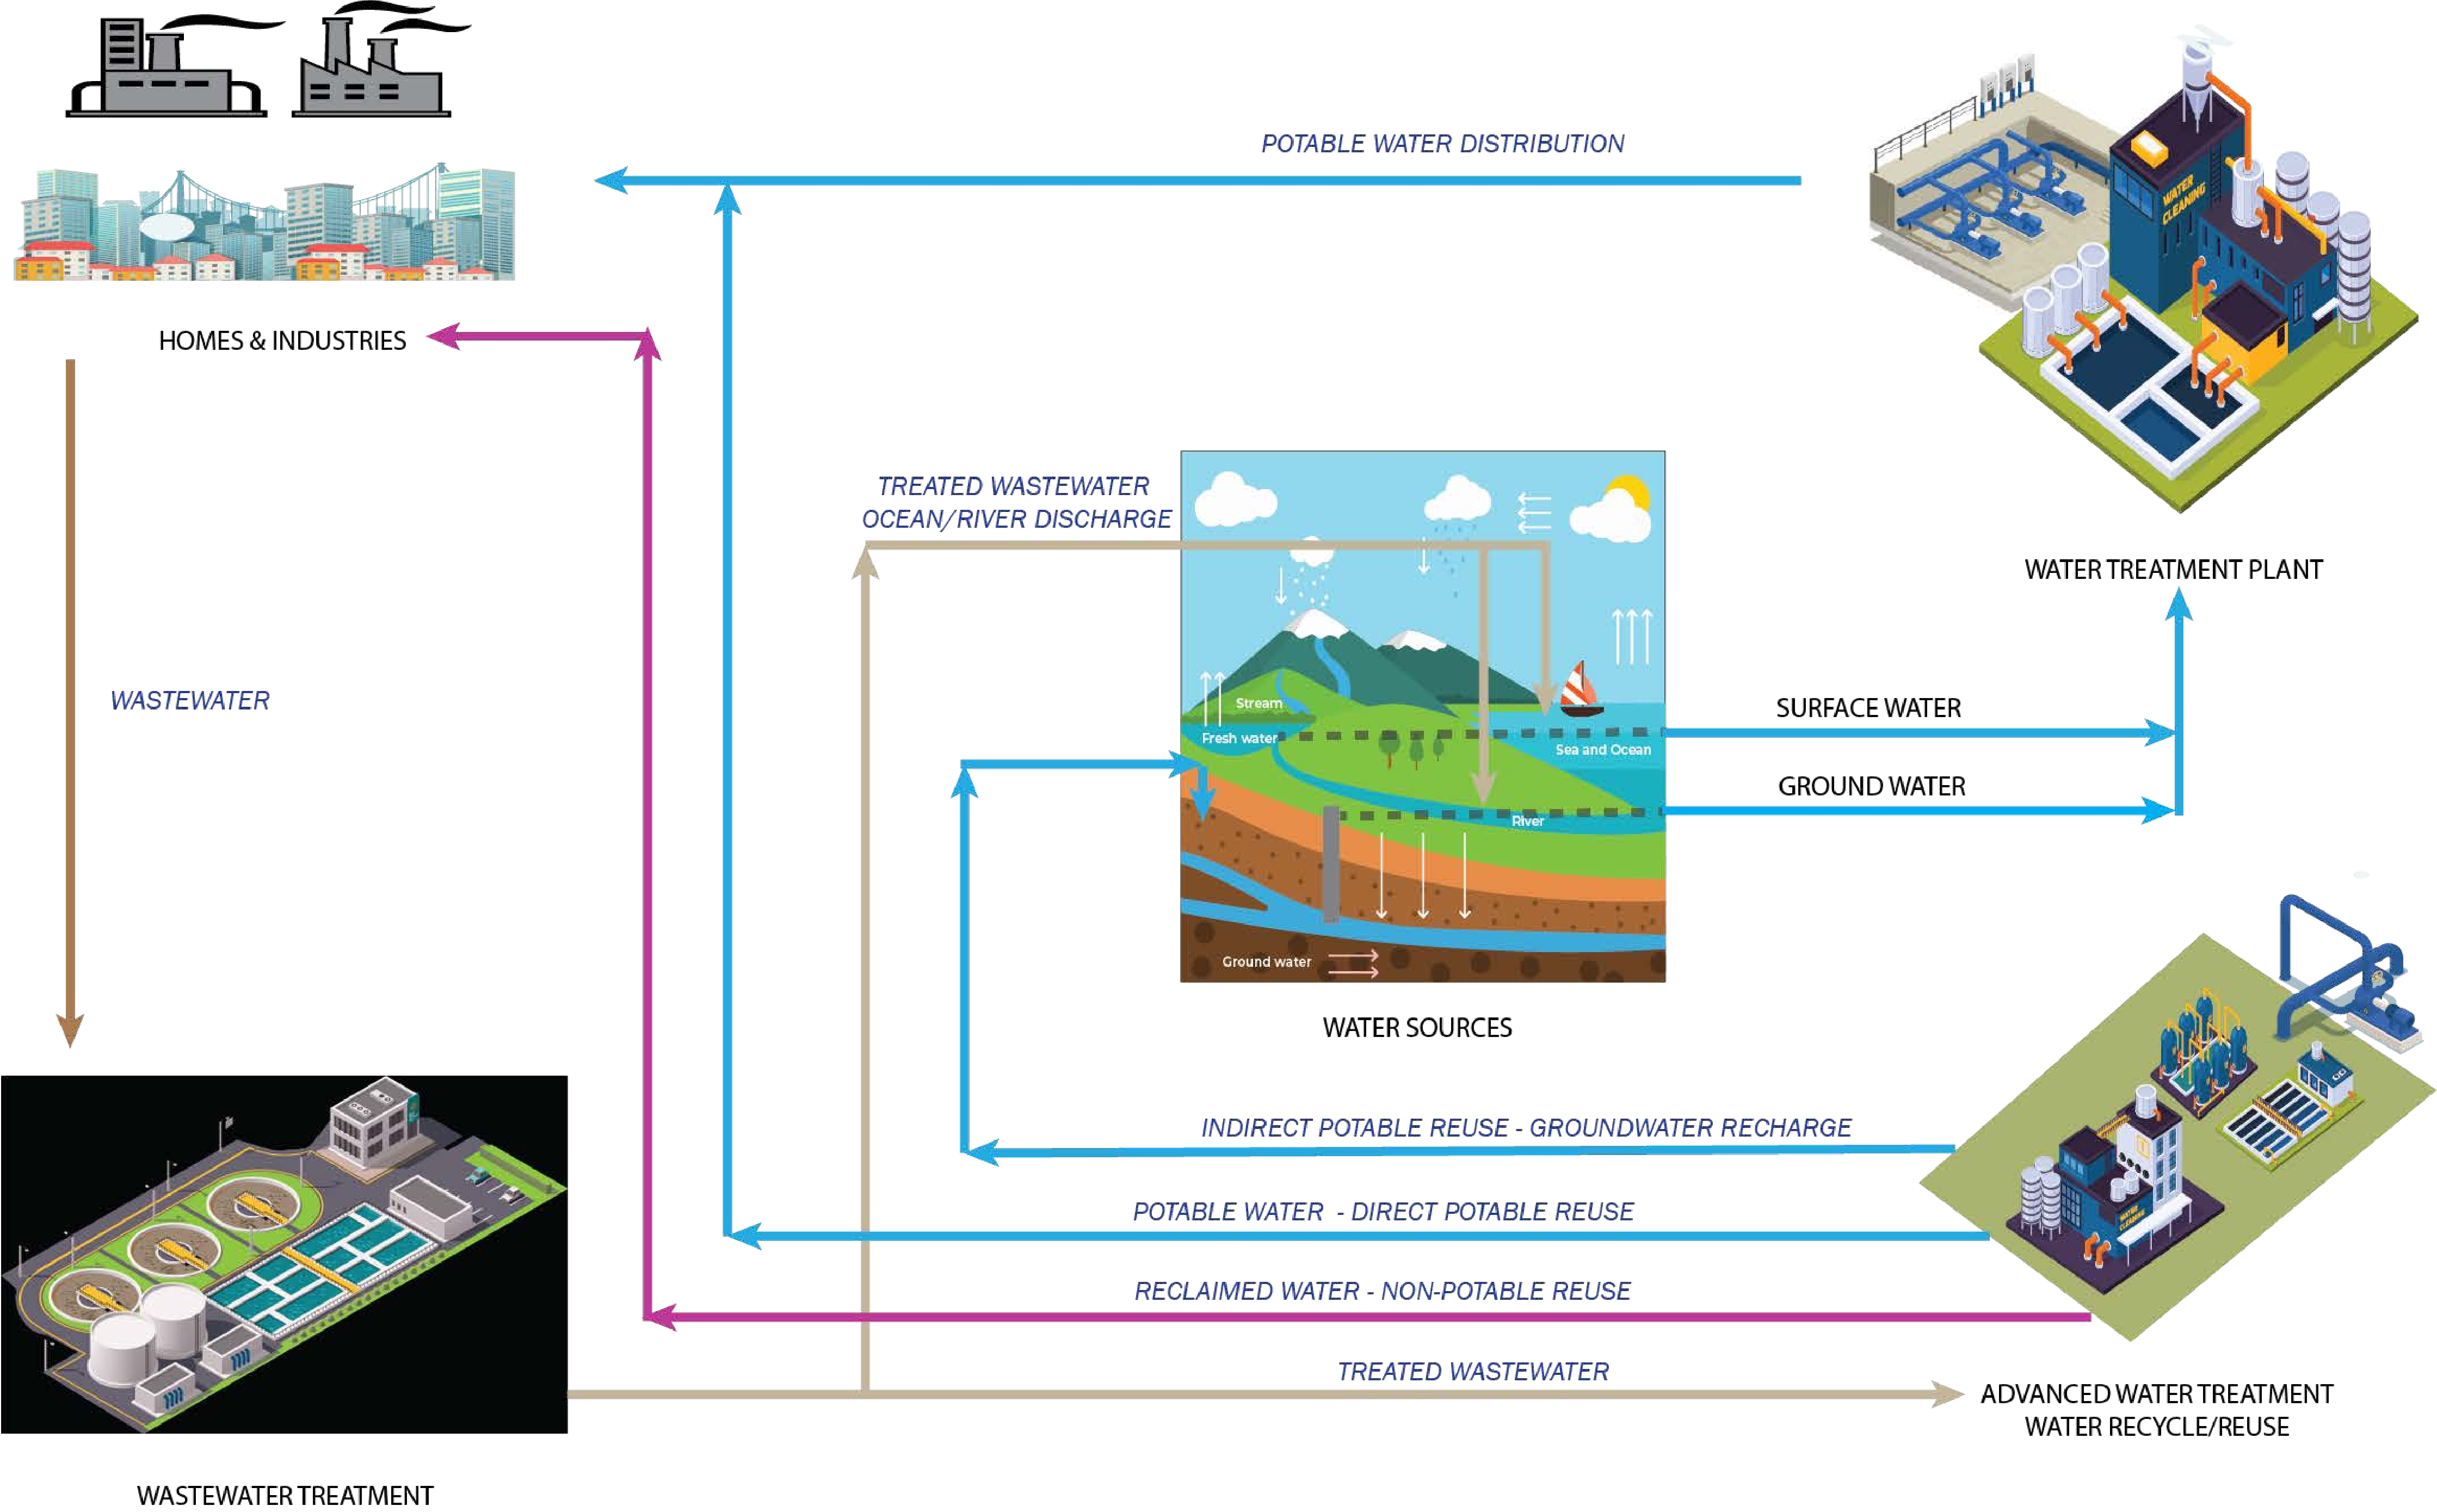
\includegraphics[scale=0.2]{Test4}\\
\captionof{figure}{Water Use - Reuse Cycle}%\caption{}
\end{figure}

\item Water reuse (also commonly known as water recycling or water reclamation) reclaims water from a variety of sources then treats and reuses it for beneficial purposes such as agriculture and irrigation, potable water supplies, groundwater replenishment, industrial processes, and environmental restoration.
\item Water reuse can provide alternatives to existing water supplies and be used to enhance water security, sustainability, and resilience.

\item Unplanned or de facto reuse refers to situations in which a source of water is substantially composed of previously-used water. An example of unplanned water reuse occurs when communities draw their water supplies from rivers, such as the Colorado River and the Mississippi River, that receive treated wastewater discharges from communities upstream.



\item Clean water is vital to our health, communities, and economy. 
\item There is no universally accepted definition of “safe drinking water.” Generally speaking, safe drinking water, is defined as the water that does not represent any significant risk to health over a lifetime of consumption.
\item The water cycle is primarily water exchange between the ocean and atmosphere
\item The amount of water that is available for use is only a very small fraction of the total amount of water in existence.
\item Water scarcity can be caused by a mix of hydrological, infrastructural, political and social issues. 
\item In developing countries, water supply and sanitation related factors cause more than 20 percent of deaths of people under age 14. Nearly
half of all people in developing countries have infections or diseases associated with inadequate water supply and sanitation.
\item Chemical contaminants in drinking water arise including arsenic, fluoride or nitrate, emerging contaminants such as pharmaceuticals, pesticides, per- and polyfluoroalkyl substances (PFASs) and microplastics generate public concern.
\item Microbiologically contaminated drinking water can transmit diseases such as diarrhoea, cholera, dysentery, typhoid and polio and is estimated to cause 485 000 diarrhoeal deaths each year.
\item The amount of water that is available for sustenance including agriculture, sanitation and hygiene is limited in many areas of the world.  Billions of people throughout the world are battling daily against enormous difficulties accessing the most basic services.\\
\item Some 1.1 billion people worldwide lack access to water, and a total of 2.7 billion find water scarce for at least one month of the year.
\item Inadequate sanitation is also a problem for 2.4 billion people—they are exposed to diseases, such as cholera and typhoid fever, and other water-borne illnesses. Two million people, mostly children, die each year from diarrheal diseases alone.\\
\item Many of the water systems that keep ecosystems thriving and feed a growing human population have become stressed. Rivers, lakes and aquifers are drying up or becoming too polluted to use. More than half the world’s wetlands have disappeared.
\item Climate change is altering patterns of weather and water around the world, causing shortages and droughts in some areas and floods in others, changing large-scale hydrological cycle.\\
\item At the current consumption rate, this situation will only get worse. By 2025, two-thirds of the world’s population may face water shortages. And ecosystems around the world will suffer even more\\
\item Factors affecting water supplies include:
\begin{enumerate}
\item Pollution\\
Surface waters - streams, rivers, lakes which may be the source of drinking water supply are easily contaminated by agricultural and urban runoffs with fertilizer, pesticides, oil, dirt, bacteria and other pollutants.\\
\vspace{0.2cm}
Even groundwater is not safe from pollution, as many pollutants can leach into underground aquifers. Some effects are immediate, as when harmful bacteria from human waste contaminate water and make it unfit to drink or swim in.\\
\vspace{0.2cm}
Even trace levels of heavy metals, dyes, and microbes are hazardous to human health, aquatic systems, and the environment.\\
\vspace{0.2cm}
In other instances—such as toxic substances from industrial processes—it may take years to build up in the environment and food chain before their effects are fully recognized.\\
\begin{figure}[htp]
\begin{center}
%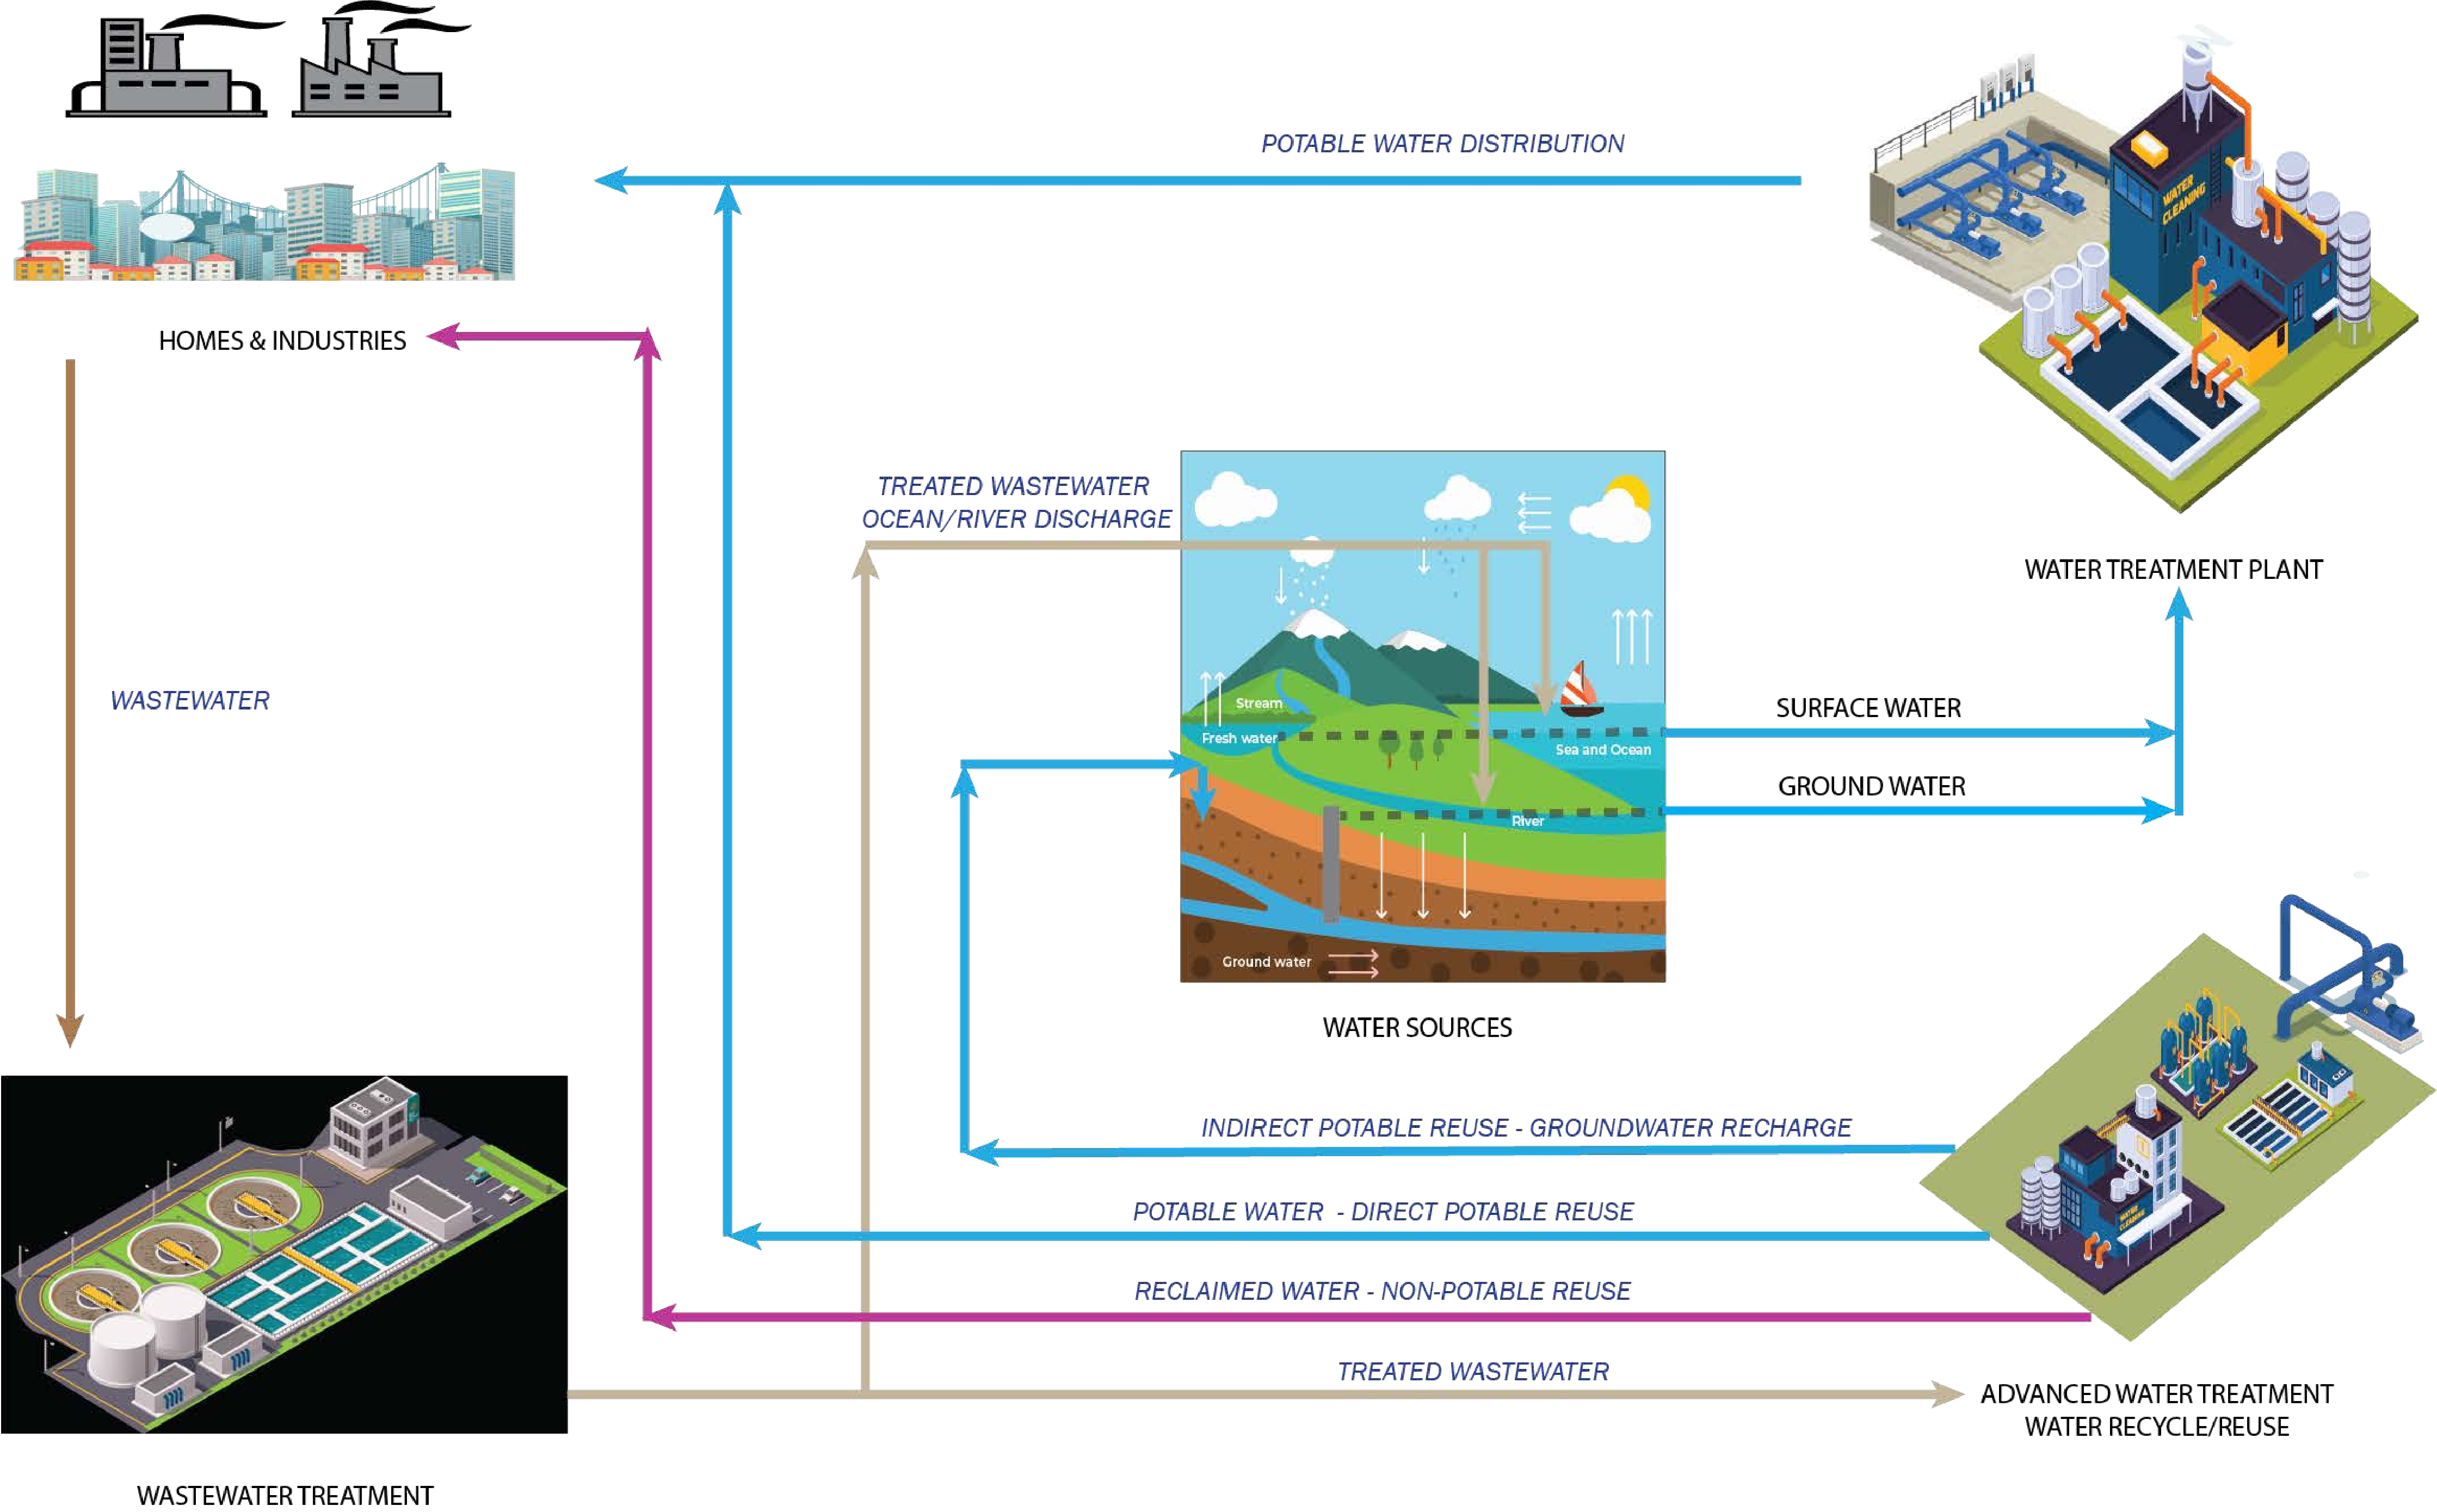
\includegraphics[landscape=true]{Test4.pdf}
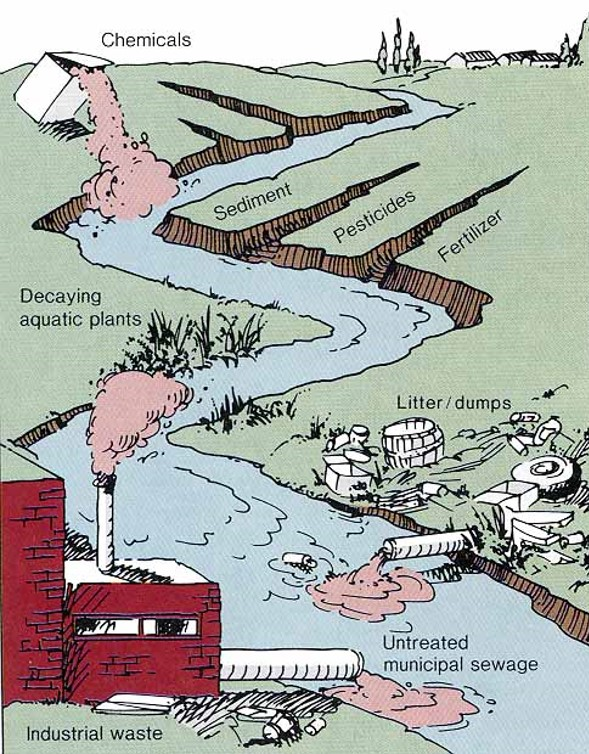
\includegraphics{WaterContamination}\\
\captionof{figure}{Water Contamination}
\end{center}
\end{figure}


\item The state’s water supplies are from surface water sources such as rivers, streams, and lakes and from groundwater sources, which are present in groundwater basins throughout the state. The amount of drinking water derived from surface water sources versus groundwater sources can vary annually depending on rainfall and snowpack conditions. In general, surface water sources provide a larger portion of the drinking water supply than
\item groundwater sources; however, 90 percent of the public water systems only have groundwater. For example, the United States Geological Survey (USGS) estimated that, in 2015 in California, 54 percent of the drinking water provided by public water systems was from surface water sources (https://pubs.er.usgs.gov/publication/cir1441). This is down dramatically from the 2010 report, were it was over 80 percent of the state’s drinking water was from surface water sources. This change may be due to drought conditions, which significantly increases reliance on groundwater sources. Table 3-1 shows over 90 percent of the source drinking water facilities are groundwater wells.
\item As most of the surface water sources are already allocated, additional water needs have been met through groundwater sources. Historically, the use of groundwater was not regulated. As demand for groundwater continued to increase, effective management was needed to protect the future availability and quality of the supply. In September 2014, Governor Edmund G. Brown Jr. signed a three-bill package known as the Sustainable Groundwater Management Act (SGMA). The legislation allows local agencies to adapt groundwater sustainability plans to their regional economic and environmental needs. The Act creates a framework for sustainable, local groundwater management for the first time in California history. The primary responsibility assigned to the State Water Board is to protect groundwater resources if a local agency cannot or will not manage its groundwater sustainably. If local efforts fail to adequately manage groundwater, the State Water Board has the authority to step in and collect groundwater data, designate the basin as probationary, develop groundwater management plans, and collect fees for these activities. 
\item Over-extraction of groundwater to meet community and agricultural needs, particularly during times of drought, can reduce the availability of this important source of drinking water. Monthly monitoring of both the static and pumping water levels will provide information on the effects of drought-related and overdrafting stresses on groundwater sources. The California Water Plan Update 2018 points out the significance of groundwater withdrawal, particularly to the Central Valley, where most of California’s groundwater extraction occurs (https://water.ca.gov/Programs/California-Water- Plan/Update-2018).
The loss of groundwater can lead to increased pumping costs to access water from greater soil depths. In addition, groundwater loss from its aquifers can result in land subsidence, which can damage water-related infrastructure such as canals, resulting in water loss. The associated collapse of the hydrogeological structure of aquifers is problematic for their ability to rehydrate, and can interfere with the functionality of drinking water wells. A 2019 DWR press release on subsidence in the Sacramento Valley presents an example of the problems that subsidence presents
\item Alternative or Supplemental Sources of Drinking Water
In addition to the usual surface and groundwater sources of drinking water, there are alternative or supplemental sources of water, which may be used to augment drinking water supplies. These include recycled water and desalination, which may be used to treat seawater or brackish groundwater.
\begin{itemize}
\item Recycled Water\\
There has been considerable development in the use of recycled water to supplement drinking water supplies. Recycled water is obtained from municipal wastewater (sewage)
treatment plants and is treated prior to its reuse. It is likely that recycled water will become a more significant source of drinking water in some areas of California.
Recycled water may be used as an indirect source of drinking water (called indirect potable reuse), wherein recycled water is used to augment groundwater or surface water sources, by being introduced into those sources after additional treatment and prior to further treatment before it is made available for consumption by drinking water customers.
Most of the indirect potable reuse water activity to date has been in Orange County, in San Bernardino County, and in Los Angeles County, where recycled water has been highly treated and reintroduced to groundwater by direct injection or by the use of recharge basins, from which the recycled water percolates into underground aquifers. New projects are also planned in Monterey County. In addition, the City of San Diego is planning a surface water augmentation project. San Diego has extensively studied the use of highly treated recycled water to supplement its surface water drinking water supplies.
Indirect potable reuse projects operate under permits issued by the Regional Water Boards, who consult with DDW to establish conditions necessary to protect drinking water supplies. In addition, the State Water Board now has authority to issue indirect potable reuse permits.
To assist in the development of recycled water projects for groundwater replenishment that are protective of public health, regulations for such projects were adopted and became effective on June 18, 2014.
Since the 2015 Plan, as required by Chapter 700, Statutes of 2010 (SB 918), the State Water Board adopted regulations for surface water augmentation in December 2016. These regulations were developed following the findings of the Expert Panel formed pursuant to SB 918 that such regulations would be protective of public health for this use. The regulations are found at the DDW website mentioned above.
Recycled water is also being considered as a direct source of drinking water, which would be introduced directly into a public water system’s distribution system for customer use (direct potable reuse). Under SB 918 and SB 322 (Chapter 637, Statutes of 2013), the State Water Board was required to investigate and report on the feasibility of developing uniform water recycling criteria for direct potable reuse. A report to the legislature was submitted in December 2016; it concluded that the development of such criteria was feasible, but that there were significant data gaps and research needs to ensure adequate public health protection.
Use of alternative water supplies such as indirect potable reuse for groundwater replenishment and surface water augmentation for drinking water requires considerable treatment to provide adequate public health protection. Care must be taken to ensure the required high level of water treatment does not fail, so customers do not receive unsafe
drinking water. For direct potable reuse projects, where the connection between highly treated wastewater and treated drinking water is more proximal and immediate than it is in indirect potable reuse projects, more treatment and highly focused operations will be required for the protection of public health.
The purpose of current and potential future State Water Board water recycling regulations is to ensure that project design, construction, and operation are protective of public health. \\
In 2019, the State Water Board completed a revision to the Framework (Framework Second Edition) to reflect the State Water Board’s current thinking on regulating direct potable reuse. The Framework Second Edition includes a discussion of the regulatory approach for direct potable reuse, as well as an update on the consideration of drinking water treatment plants. The Framework Second Edition is presented in a format that highlights the revisions that were made.
\item Desalination
Desalination of water that is otherwise not fit for consumption may provide another source of supplemental water supply. Typically, desalination is either categorized as seawater or brackish water desalination. Seawater desalination treats ocean water obtained from either an open water intake or a subsurface intake to a treatment plant is located near the coast, Brackish water desalination treats groundwater with elevated salt levels and can occur in both inland and coastal areas.
There are four seawater desalination facilities in California that produce drinking water. The permitted seawater desalination facilities are shown in Table 3-2. Other coastal counties have proposed desalination facilities but have not yet begun construction.
\end{itemize}

\begin{table}[]
\begin{tabular}{|l|l|l|}
\hline
Desalination   Project                                   & Production                                 & County   Served           \\ \hline
Claude   "Bud"   Lewis   Carlsbad   Desalination   Plant & 56,000   acre-ft   per   year   (50   MGD) & San   Diego               \\ \hline
Charles   E.   Meyer   Desalination   Plant              & 3,125   acre-ft   per   year   (2.8 MGD)   & Santa   Barbara           \\ \hline
Santa   Catalina   Island   Desalination   Plant         & 364   acre-ft   per   year   (0.33   MGD)  & Santa   Catalina   Island \\ \hline
Sand   City   Coastal Desalination   Plant               & 336   acre-ft   per   year   (0.30   MGD)  & Monterey                  \\ \hline
\end{tabular}
\caption{Permitted De-Salination Facilities in California}
\end{table}



\begin{table}[]
\begin{tabular}{|l|l|}
\hline
Water   Source                                                  & Number   of   Facilities \\ \hline
Surface   Water                                                 & 939                      \\ \hline
Groundwater   under   direct   influence   of   surface   water & 281                      \\ \hline
Groundwater                                                     & 15,041                   \\ \hline
\end{tabular}
\caption{Water System Facilities (2020 Data)}
\end{table}



\item Water supply diversion for agriculture and energy production\\
Agriculture uses 70\% of the world’s accessible freshwater.  Water diversions for agriculture usage, for supplying urban populations and for energy generations have significantly affected local water supplies both for human consumption and for sustaining the natural habitat and ecosystems.

\item Population growth\\
In the last 50 years, the human population has more than doubled. This rapid growth — with its accompanying economic development and industrialization—has transformed water ecosystems around the world and resulted in a massive loss of biodiversity.
\vspace{0.2cm}
The population increase exercises Concern about water availability grows as freshwater use continues at unsustainable levels. Furthermore, these new faces also need food, shelter, and clothing, thus resulting in additional pressure on freshwater through the production of commodities and energy.\\

\item Climate change\\
Climate change increases the odds of worsening drought in many parts of the world. In many places, droughts are expected to get more frequent, intense, and longer lasting.\\

How climate change contributes to drought:\\

\begin{itemize}
\item Warmer temperatures enhance evaporation, making periods with low precipitation drier than they would be in cooler conditions.
\item Climate change alters the timing of water availability. Warmer winter temperatures are causing less precipitation to fall as snow resulting in a decreased snowpack which:
\item Impact water management systems which rely on spring snowpack melt
\item Impact certain ecosystems which depend on snow melt to supply cold water for species like salmon. 
\item Exacerbates drought because of because of increases surface temperatures caused by a decreased reflective surface of the snow.
\item Warming increases precipitation variability, meaning there will be more periods of both extreme precipitation and drought. This creates the need for expanded water storage during drought years and increased risk of flooding and dam failure during periods of extreme precipitation.\\
\end{itemize}
\end{enumerate}


\begin{figure}
\begin{center}
\includegraphics[scale=0.5]{WaterSources}\\
\captionof{figure}{Water Supply Sources}%\caption{}
\end{center}
\end{figure}
\begin{enumerate}
\item Groundwater
\begin{itemize}
\item Groundwater is considered to be water that is below the earth’s crust, but not more than 2500 feet below the crust. Water between the earth’s crust and the 2500-foot level is considered usable fresh water.\\

\item A watershed is an area of land that contributes water to a given location, such as a reservoir, a confluence of two streams, or the ocean. Within a watershed, water from rain or snow flows down the slope, through the soil, or via groundwater flow – and usually by a combination of these routes – to reach the stream and contribute to the flow of the stream. Watersheds are
important sources of drinking water, as well as a habitat for many aquatic species. Healthy watersheds with intact native vegetation and wetlands provide important functions such as water purification, flood control, nutrient recycling, and groundwater recharge.

\item An aquifer is a body of porous rock or sediment saturated with enough groundwater that it can be pumped to the surface and used for drinking water, irrigation, industry, or other uses. . Groundwater enters an aquifer as precipitation seeps through the soil. It can move through the aquifer and resurface through springs and wells.

\item Where groundwater can move rapidly, such as through gravel and sandy
deposits, an aquifer can form.  

\item There are two general types of aquifers: confined and unconfined. Confined aquifers have a layer of impenetrable rock or clay above them, while unconfined aquifers lie below a permeable layer of soil.

\item A common misconception about aquifers is that they are underground rivers or lakes. While groundwater can seep into or out of aquifers due to their porous nature, it cannot move fast enough to flow like a river. The rate at which groundwater moves through an aquifer varies depending on the rock’s permeability.

\item Much of the water we use for domestic, industrial, or agricultural purposes is groundwater. Most groundwater, including a significant amount of our drinking water, comes from aquifers. In order to access this water, a well must be created by drilling a hole that reaches the aquifer. While wells are manmade points of discharge for aquifers, they also discharge naturally at springs and in wetlands.

\item Groundwater can become depleted if we use it at a faster rate than it can replenish itself. The replenishment of aquifers by precipitation is called recharging. Depletion of aquifers has increased primarily due to expanding agricultural irrigation. Groundwater can become contaminated when an excessive amount of pesticides and herbicides are sprayed on agricultural fields, septic tanks leak, or landfills are improperly lined or managed and toxic materials seep through the soil into the aquifer.

\item Aquifers naturally filter groundwater by forcing it to pass through small pores and between sediments, which helps to remove substances from the water. This natural filtration process, however, may not be enough to remove all of the contaminants.

\item Groundwater is obtained from the following:\\
\begin{itemize}
\item Wells
\item Springs that are not influenced by surface water or a local hydrologic event
\item When a well or spring is influenced by an adjacent surface water source or by a local hydrological event, the supply is said to be groundwater under the direct influence of surface water (GUDISW).
\end{itemize}
\item Advantages of groundwater with respect to surface water:\\
\begin{itemize}
\item Groundwater is not as easily contaminated as surface water.
\item The quality of groundwater, while not always as good as would be preferred, is stable throughout the year.
\item Groundwater sources are generally lower in bacteriological count than surface water sources.
\item Groundwater is available in most locations throughout the continental US and Alaska.
\end{itemize}
\item Disdvantages of groundwater with respect to surface water:\\
\begin{itemize}
\item Once a groundwater source is contaminated, it is difficult for it to recover. There is no easy way to remove the contaminants.
\item Groundwater usually contains more minerals than surface water, including increased levels of hardness. Because groundwater is in contact longer with minerals, there is more time to bring them into solution.
\item Removal of groundwater normally requires a pump, thus increasing operation cost.
\item Groundwater is more susceptible to long-term contamination from fuel spills.
\item Groundwater supplies often have high levels of iron and manganese, thus increasing treatment cost and/or causing stains on plumbing and the clothing of customers.
\item Wells in the coastal areas are subject to salt water intrusion into the aquifer20
and well. This contamination is difficult to predict and costly to treat.
\item Sources of contamination can be hidden from sight.
\end{itemize}
\end{itemize}

\item Surface water\\
\begin{itemize}
\item Surface water is water that is open to the atmosphere and results from overland flow. It is also said to be the result of surface runoff 3. These are two ways of saying the same thing.
\item Examples of surface water include:
\begin{itemize}
\item Streams, Rivers, Lakes
\item Man-made impoundments - Reservoirs
\item Wells drilled next to or in a stream or river
\item Rain catchments
\end{itemize}

\item Advantages of surface water with respect to groundwater:
\begin{itemize}
\item It is easily located. It takes no sophisticated equipment to find a surface water source.
\item In many parts of the US, considerable data is available on quantity and quality of existing surface water supplies.
\item Surface water is generally softer than groundwater, which makes treatment much simpler.
\end{itemize}
\item Disadvantages of surface water with respect to groundwater:
\begin{itemize}
\item Surface waters can be easily contaminated with microorganisms that cause waterborne diseases and chemicals that enter the stream from surface runoff and upstream discharges.
\item The turbidity of a surface water source often fluctuates with the amount of precipitation. Increases in turbidity increase treatment cost and operator time.
\item The temperature of surface water fluctuates with the ambient temperature. This makes it difficult to produce consistent water quality at a water treatment plant.
\item The intake structure may become clogged or damaged from winter ice, or the source may be so shallow that it completely freezes in the winter. This is a common problem with surface water sources in the arctic.
\item Removing surface water from a river, lake, or reservoir requires a legal right, referred to as a water right. 
\item Using surface water as a source means that the purveyor is obligated to meet the requirements of the Surface Water Treatment Rule (SWTR) of the State Drinking Water Regulations. This rule requires that, in most instances, any surface water source must have a filtration system.
\item Surface waters that are high in color, especially color that is the result of decaying vegetation, have the potential to produce high levels of Total Trihalomethanes (TTHM). These chemical compounds are formed when chlorine is added to the water. The problem with the TTHM is that some of them are carcinogenic (can cause cancer) and are referred to as disinfection by-products (DBP).
\end{itemize}
\end{itemize}
\end{enumerate}

In the United States, 9 out of 10 people get their water from one of more than 148,000 public water systems. To make sure water from these systems is safe to drink, federal, state, and local authorities regulate and monitor public water systems.\\

\begin{figure}
\begin{center}
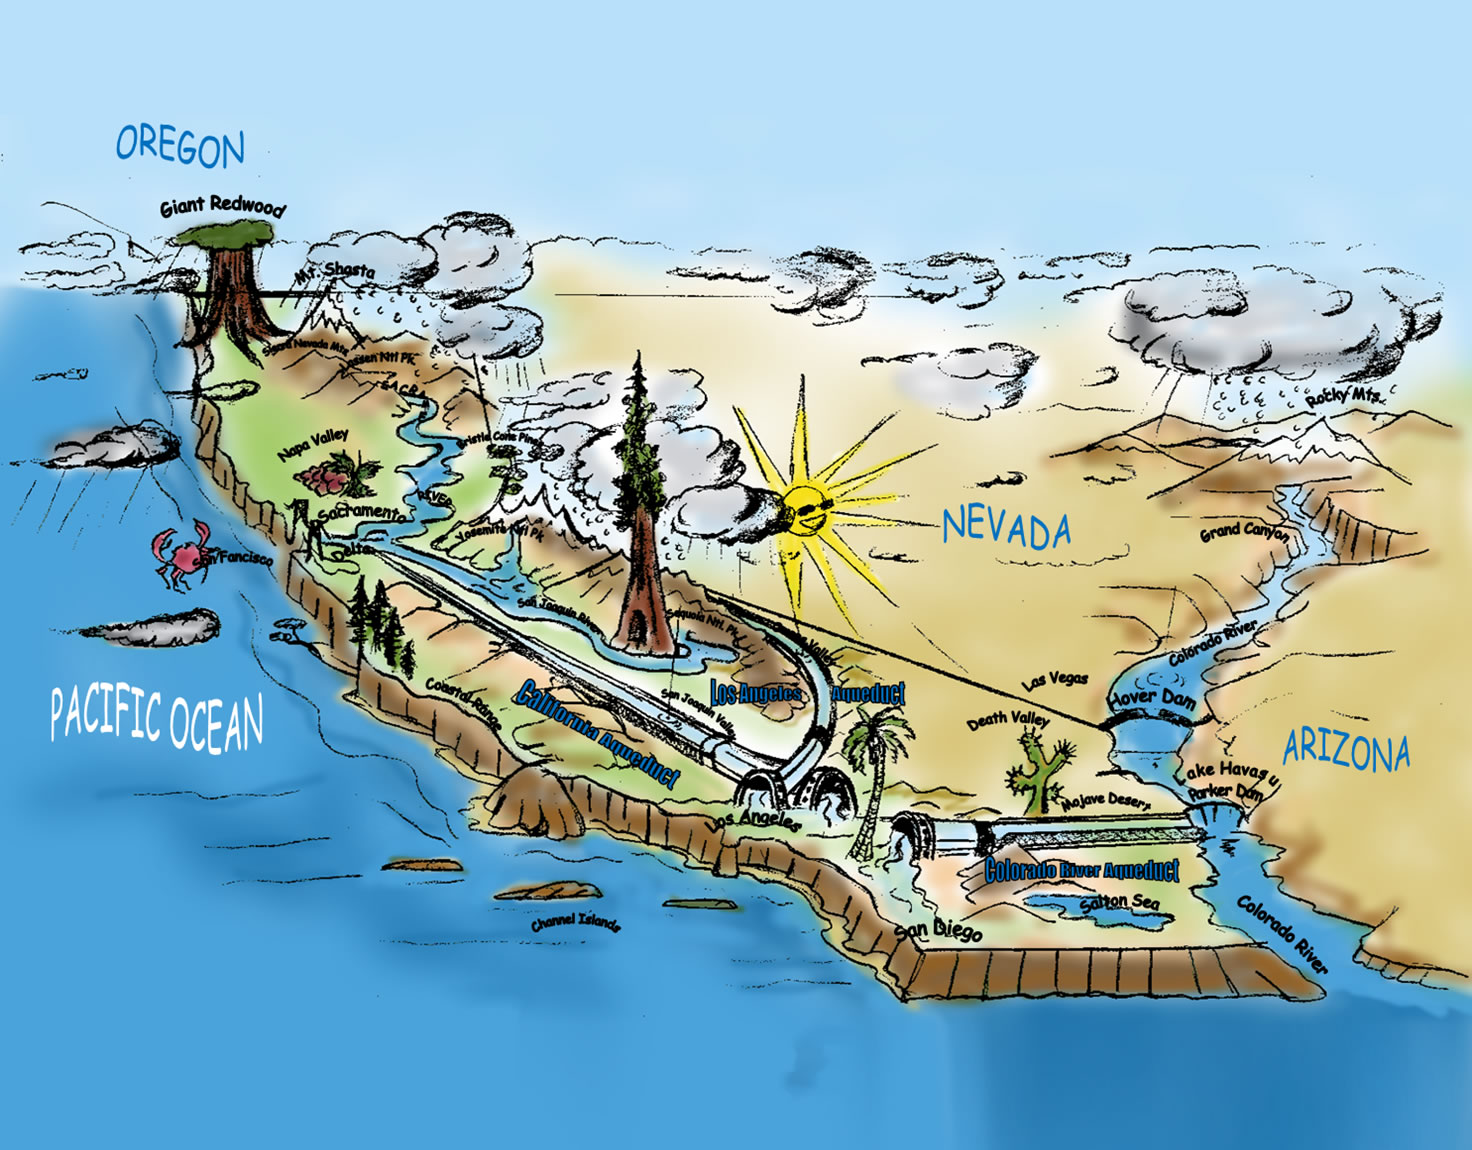
\includegraphics[scale=0.24]{waterSupplyIllustration1}\\
\captionof{figure}{Southern California Water Supply Illustration}%\caption{}
\end{center}
\end{figure}

\begin{figure}
\begin{center}
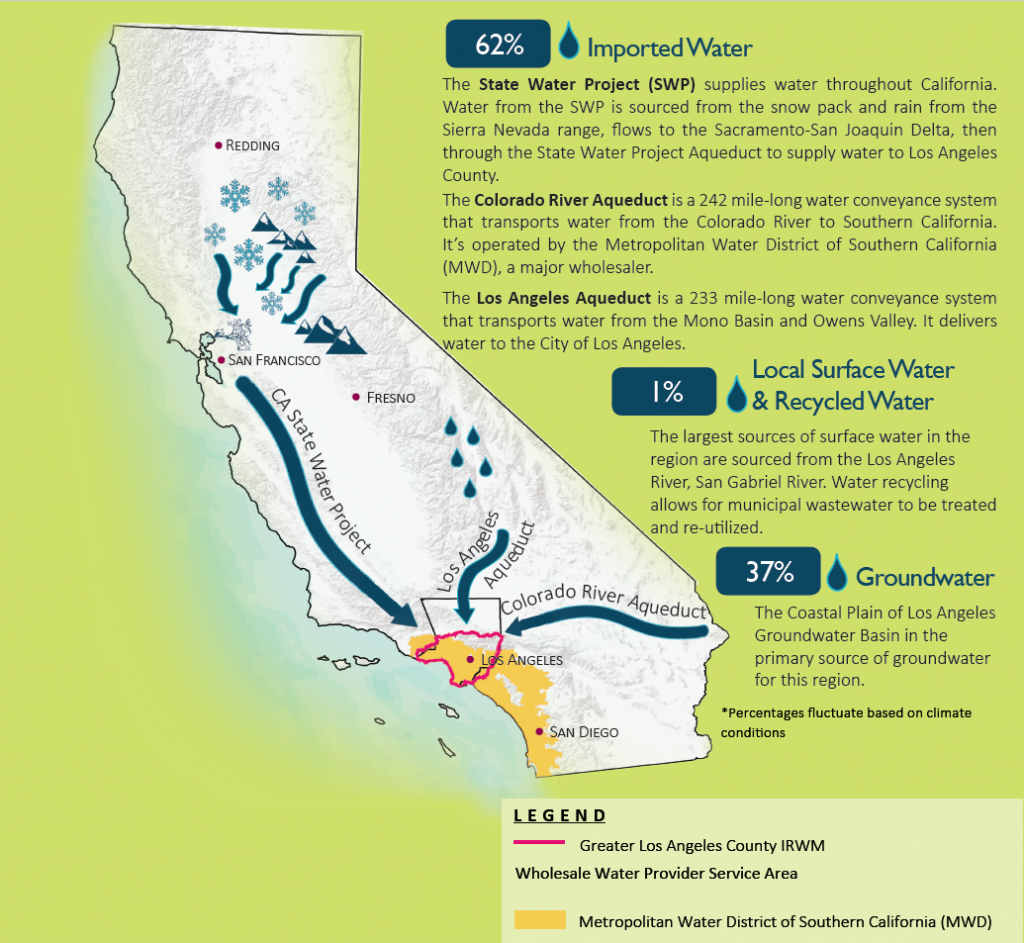
\includegraphics[scale=0.40]{LosAngelesWaterSupply}\\
\captionof{figure}{Los Angeles County Water Supply Sources}%\caption{}
\end{center}
\end{figure}

California primarily relies on a mixture of surface water and groundwater supplies for drinking water. The balance of supplies used in a given year is dependent upon the region of the state, water needs, water resource availability, and long-term weather conditions within the state. During periods of normal to high rainfall, surface water sources make up a higher percentage of the overall drinking water supplies across the state. However, use of groundwater increases and surface water supplies are strained during periods of lower than average rainfall.\\


The California State Water Project (SWP):\\

Managing water remains one of the great challenges for California. Population growth, a shifting climate, and declining ecosystem health are putting pressure on the state’s water supply and flood management systems.\\

 is a multi-purpose water storage and delivery system that extends more than 705 miles -- two-thirds the length of California. A collection of canals, pipelines, reservoirs, and hydroelectric power facilities delivers clean water to 27 million Californians, 750,000 acres of farmland, and businesses throughout our state.\\

 Such valuable
functions are sometimes referred to as “ecosystem services” (Revenga et al. 1998).\\
Californians rely on both surface and ground water sources for their domestic water supply. Unfortunately, the watersheds that yield water to these sources face many sources of degradation including sedimentation and pollution from residential and industrial development, timber harvests, agricultural production, land clearing, and mining (Revenga et al. 1998, Bolund and Hunhammar 1999). While these types of degradation can affect both surface
and groundwater, this report focuses on surface drinking water sources and watersheds. However, protecting and/or restoring native vegetation in these watersheds can also improve groundwater supply by maintaining or increasing groundwater recharge rates.\\
Mapping the watersheds that supply drinking water to people is a crucial first step to ensure they remain healthy and protected. Previous studies have listed sources or mapped a subset of the watersheds (e.g., the watersheds for one city), but none of these explicitly mapped all 
watersheds that supply drinking water to Californians1
\end{itemize}
\section{Cost of Water}\index{Cost of Water}
\begin{itemize}
\item Water costs have, on average over a five- year period from 2012 to 2017, increased about 35 percent within all size groups of water systems (range of 23 to 40 percent). \item Average water costs remain highest in the San Francisco Bay Area, Central Coast, and Southern California, and lowest in the Central Valley/Agricultural (including Imperial County), Foothill, and Mountain/Desert regions. 
\item On average, customers of small water systems (PWS serving fewer than
200 service connections) pay approximately 21 percent more for water than those customers served by larger systems.
\item Many economically disadvantaged communities are served by small water systems. As a result, water affordability has become a significant issue among residents in these communities.

\item Small water systems continue to have the largest percent of water quality problems and the highest rate of noncompliance with drinking water standards. In particular, small water systems serving between 15 and
200 service connections have the greatest noncompliance rates, especially those that serve disadvantaged communities.
Many of these small water systems lack the necessary resources to comply. 

\item There are more than 1,300 State Small water systems servicing about 32,000 people. Many of these systems are vulnerable to the same problems that small public water systems confront. However, State Small water system requirements are much less strict than those placed on PWS and those systems are not subject to addressing water quality problems unless they become PWS.

\end{itemize}

\section{Drinking Water Regulations}\index{Drinking Water Regulations}
\begin{itemize}
\item Timeline of key legislation on regulating water quality is given below.
\begin{enumerate}
\item 1893 – U.S. Public Health Service (USHPS) enacts Interstate Quarantine Act, a regulation prohibiting use of a common drinking cup by passengers on commercial transportation carriers traveling between states.
\item 1914 - Federal standard for bacteriological water quality developed.
\item USPHS expanded standards to include guidelines for bacteriological sampling and maximum levels for lead, fluoride, arsenic, selenium, and chromium. Generally, these were non-enforceable guidelines.
\item 1962 – Guidelines are expanded to include additional constituents. Limits on many constituents made mandatory.
\item 1974 – Congress passes Safe Drinking Water Act.
\item 1986 and 1996 - Safe Drinking Water Act amended.
\end{enumerate}

\item United States Environmental Protection Agency (EPA)  is mandated by Congress through the Safe Drinking Water Act to establish drinking water regulations and periodically review these regulations to update them.

\item EPA studies health issues related to water quality and develops regulations, standards, and guidance documents related to drinking water. It legislates specific minimum requirements that the states must meet, though the states are generally permitted to enact more stringent requirements.

\item The United States Environmental Protection Agency (EPA) defines a Public Water System as “a system for the provision to the public of water for human consumption through pipes or other constructed conveyances, if such system has at least fifteen service connections or regularly serves an average of at least twenty-five individuals daily at least 60 days out of the year.”

\item Each Public Water System is required to have domestic water supply permits and is responsible for providing affordable, safe drinking water to their customers 24 hours a day, 7 days a week, 365 day a year.

\item All public water systems are subject to the same health based standards and laws whether they are a big city, a small community, or a rural restaurant. However, there are some minor adjustments that are made to monitoring frequencies based on population and water system type.

\item Requirements of a Public Water Agency in California include:

\begin{itemize}

\item Permitting engineering and technical reports, including pump tests, at least two water supply well sources for communities, a 50-foot radius source protection zone around all new wells, a minimum of a 50-foot annular seal on new wells , a well flow meter and initial monitoring \\
\item  Construction, including elevated storage or backup electricity for pumps to maintain 40 pounds per square inch (psi) minimum pressure at all times, proper construction of distribution systems, adequate storage capacity and fire fighting capacity \\
\item  As-built maps.\\
\item  Annual water-treatment chemicals and equipment for distribution monitoring of any added chemical treatment (dependent on the type of needed treatment) \\
\item  Ongoing raw water chemical monitoring sampling and analysis. \\
\item  Ongoing raw water bacteriological monitoring sampling and analysis. \\
\item  Ongoing treated water bacteriological monitoring sampling and analysis.\\
\item  Maintenance of bacteriological plans and emergency notification plans for water quality emergencies . \\
\item  Ongoing lead and copper monitoring including sampling and analysis and maintenance of a lead and copper plan. \\
\item  Ongoing disinfection byproducts monitoring and maintenance of an associated plan.\\
\item  Maintaining a customer water quality complaint program.\\
\item  Main flushing, valve and meter maintenance, and maintaining system maps.\\
\item  Cross connection program and annual back-flow device testing.\\
\item  Licensed water treatment operator and distribution staff.\\
\item  Written procedures for system maintenance, for example pipeline break procedures, etc.\\
\item  Source capacity planning studies and permit amendments for any additional growth.\\
\item  Annual Consumer Confidence Report preparation and distribution. Requirements continue on next page.\\
\item  Annual Electronic Report submittal to State Water Resource Control Board-Division of Drinking Water \\
\item  Records of the estimated life of all pumps, treatment, storage, and distribution system and an annual capital improvement plan to fund infrastructure replacement.\\
\item  Metering and billing staff.\\
\item  Emergency reserves for drought, regulatory changes, public notice of bacteriological or chemical failures, etc. (CHSC §116540) \\
\item  Maintaining of business licenses, annual drinking water permit fees and payment of any State enforcement fees for actions resulting from water system non-compliance .\\
\item  Appropriate working area for staff, chemicals, and records \\
\item  Insurance and liability for staff, with duties including climbing tanks, handling hazardous chemicals, etc. \\
\item  Management staff that is knowledgeable about drinking water. Staff coordinate the above and maintain financial controls.\\
\item  If the source is surface water, there may be additional requirements: o A water treatment plant meeting all Surface Water Treatment Rule requirements  Continuous operator supervision of the water treatment plant when in service o Chemical monitoring equipment, at minimum turbidity and chlorine  o Operations Plan and Alarms. Monthly monitoring reports to the Division of Drinking Water o Additional raw water sampling requirements.



\end{itemize}

\item Different types of water systems have different treatment requirements. Water systems are classified on this basis. Regulatory requirements vary from one class to another, and operator certifications are specific to certain classifications of systems.

\item Types of Public Water Systems
\begin{enumerate}
\item Community Water Systems:\\
These include city, county, regulated utilities, regional water systems and even small water companies and districts where people live.  The Community Water Systems can be either:
\begin{enumerate}
\item Small Water Systems - Water systems that serve 3,300 persons or fewer.
\item Large Water Systems - Water systems that serve more than 3,300 people.  For certain specific regulations, a system must serve more than 10,000 people or 50,000 to be considered a “Large Water System.”  Large water systems have to meet more stringent monitoring requirements under certain regulations.
\end{enumerate}

\item Noncommunity Water Systems:\\
The Noncommunity water system include:
\begin{itemize}
\item Nontransient water systems are places like schools and businesses that provide their own water. The same people have a regular opportunity to consume the water, but they do not reside there.

\item Transient water systems include entities like rural gas stations, restaurants and State and National parks that provide their own potable water source.  Most people that consume the water neither reside nor regularly spend time there.
\end{itemize}
\end{enumerate}

\end{itemize}


%\section{Drinking Water Conveyance and Distribution}\index{Drinking Water Conveyance and Distribution}
%\section{Microbiological Drinking Water Parameters}\index{Microbiological Drinking Water Parameters}
%\section{Physical Drinking Water Parameters}\index{Physical Drinking Water Parameters}
%\section{Taste and Odor}\index{Taste and Odor}
%\section{Color}\index{Color}
%\section{Temperature}\index{Temperature}
%\section{Turbidity}\index{Turbidity}
%\section{Solids}\index{Solids}
%\section{pH}\index{pH}
%\section{Alkalinity}\index{Alkalinity}
%\section{Hardness}\index{Hardness}
%\section{Solubility}\index{Solubility}
%\section{Summary}\index{Summary}
%\section{Chemical Drinking Water Parameters}\index{Chemical Drinking Water Parameters}
%\section{Organic Chemicals}\index{Organic Chemicals}
%\section{Synthetic Organic Chemicals}\index{Synthetic Organic Chemicals}
%\section{Volatile Organic Chemicals}\index{Volatile Organic Chemicals}
%\section{Total Dissolved Solids}\index{Total Dissolved Solids}
%\section{Fluoride}\index{Fluoride}
%\section{Heavy Metals}\index{Heavy Metals}
%\section{Nutrients}\index{Nutrients}
%\section{Water Pollution}\index{Water Pollution}
%\section{Sources of Contaminants}\index{Sources of Contaminants}
%\section{Radionuclides}\index{Radionuclides}
%\section{The Chemical Cocktail}\index{The Chemical Cocktail}
%\section{Chlorine Disinfectant Byproduct Regulations}\index{Chlorine Disinfectant Byproduct Regulations}
%\section{Flocculants}\index{Flocculants}
%\section{Groundwater Contamination}\index{Groundwater Contamination}
%\section{Underground Storage Tanks}\index{Underground Storage Tanks}
%\section{MtBE and Ethanol}\index{MtBE and Ethanol}
%\section{Industrial Waste}\index{Industrial Waste}
%\section{Septic Tanks}\index{Septic Tanks}
%\section{Landfills}\index{Landfills}
%\section{Agriculture}\index{Agriculture}
%\section{Saltwater Intrusion}\index{Saltwater Intrusion}
%\section{Other Sources of Groundwater Contamination}\index{Other Sources of Groundwater Contamination}
%\section{ Drinking Water Monitoring}\index{ Drinking Water Monitoring}
%\section{Is the Water Good or Bad?}\index{Is the Water Good or Bad?}
%\section{State Water Quality Standards Programs}\index{State Water Quality Standards Programs}
%\section{Designing a Water Quality Monitoring Program}\index{Designing a Water Quality Monitoring Program}
%\section{General Preparation and Sampling Considerations}\index{General Preparation and Sampling Considerations}
%\section{Preparation of Sampling Containers}\index{Preparation of Sampling Containers}
%\section{Collecting Samples from a Stream}\index{Collecting Samples from a Stream}
%\section{Sample Preservation and Storage}\index{Sample Preservation and Storage}
%\section{Test Methods}\index{Test Methods}
%\section{Titrimetric}\index{Titrimetric}
%\section{Colorimetric}\index{Colorimetric}
%\section{Visual Methods}\index{Visual Methods}
%\section{Electronic Methods}\index{Electronic Methods}
%\section{Dissolved Oxygen and Biochemical Oxygen Demand}\index{Dissolved Oxygen and Biochemical Oxygen Demand}
%\section{Sampling and Equipment Considerations}\index{Sampling and Equipment Considerations}
%\section{Biochemical Oxygen Demand}\index{Biochemical Oxygen Demand}
%\section{Sampling and Equipment Considerations}\index{Sampling and Equipment Considerations}
%\section{Hardness}\index{Hardness}
%\section{Measuring Hardness}\index{Measuring Hardness}
%\section{pH}\index{pH}
%\section{Turbidity}\index{Turbidity}
%\section{Sampling and Equipment Considerations}\index{Sampling and Equipment Considerations}
%\section{Orthophosphates}\index{Orthophosphates}
%\section{Nitrates}\index{Nitrates}
%\section{Total Solids}\index{Total Solids}
%\section{Conductivity}\index{Conductivity}
%\section{Total Alkalinity}\index{Total Alkalinity}
%\section{Fecal Bacteria}\index{Fecal Bacteria}
%\section{Apparent Color}\index{Apparent Color}
%\section{Odor}\index{Odor}

\section{Water Treatment}\index{Water Treatment}
\begin{itemize}
\item Water is essential to life. A human can only survive 5-7 days without water. However, consuming contaminated water can cause disease and death. Water can be contaminated by:
\begin{itemize}
\item Suspended material.
\item Chemical contaminants.
\item Biological contaminants.
\end{itemize}
\item Uncontaminated natural water sources are rare. Most water sources are contaminated by:
\begin{itemize}
\item Natural impurities
\item Dissolved naturally occurring minerals and chemicals, e.g., arsenic, radon.
\item Animal waste.
\item Algae, decaying leaves, and other organic material.
\item Man-made impurities
\item Industrial waste discharges.
\item Human waste discharges, e.g., malfunctioning septic systems, and sewage treatment plant discharges.
\item Agricultural activities, e.g., soil erosion, chemical fertilizers, and animal wastes/manure.
\end{itemize}
\item For the public water supplier there are two major considerations related to water supply: Quantity and Quality.  Goal is to ensure clean, wholesome and safe water in adequate quantity to meet the demands - at a reasonable cost.

\item Water treatment is necessary to ensure availability of clean, safe, potable drinking water is essential to public health. 

In order to safeguard public health, water treatment must achieve the following objectives:
\begin{itemize}
\item Remove turbidity (suspended) material.
\item Reduce concentrations of chemical contaminants to levels low enough that they do not pose a health risk and meet or exceed regulatory requirements.
\item Remove or inactivate pathogenic protozoans, bacteria, and viruses.
\item Produce water that is clear, with no objectionable colors, odors or taste.
\item Produce water that is chemically stable, and is not corrosive to metal piping and fixtures.

\end{itemize}
\end{itemize}
\section{Water Treatment Processes}\index{Water Treatment Processes}
\subsection{Conventional Water Treatment}\index{Conventional Water Treatment}
\subsection{Screening}\index{Screening}
\subsection{Coagulation}\index{Coagulation}
\subsection{Flocculation}\index{Flocculation}
\subsection{Sedimentation}\index{Sedimentation}
\subsection{Filtration}\index{Filtration}
\subsection{Hardness Treatment}\index{Hardness Treatment}
\subsection{Disinfection}\index{Disinfection}
\subsection{Nonconventional Water Treatment Technologies}\index{Nonconventional Water Treatment Technologies}
\subsection{Fluoridation}\index{Fluoridation}
\subsection{Water Treatment of Organic and Inorganic Contaminants}\index{Water Treatment of Organic and Inorganic Contaminants}
\subsection{Aeration}\index{Aeration}
\subsection{Oxidation}\index{Oxidation}
\subsection{Adsorption}\index{Adsorption}
\subsection{Demineralization}\index{Demineralization}
\subsection{Membrane Processes}\index{Membrane Processes}
\subsection{Advanced Treatment of Wastewater to Drinking Water Quality}\index{Advanced Treatment of Wastewater to Drinking Water Quality}

\begin{table}[]
\begin{tabular}{|l|l|l|l|}
\hline
System   Size (service   Connections) & Number   of Systems & Number   of Groundwater   Treatment   Facility & Number   of Surface water   Treatment   Facility \\ \hline
\textless{}200                        & 3,170               & 4,777                                          & 1,904                                            \\ \hline
200 to   999                          & 471                 & 941                                            & 1,020                                            \\ \hline
1,000   to   10,000                   & 437                 & 1,041                                          & 1,354                                            \\ \hline
\textgreater{}10,000                  & 190                 & 517                                            & 1,613                                            \\ \hline
\end{tabular}
\end{table}


\begin{table}[]
\begin{tabular}{|l|l|l|l|l|}
\hline
Water   System   Type              & Number   of   CWS & Median   population served & Number   of CWS   with violations & Average   Number   of violations   per   CWS6 \\ \hline
All CWS                            & 2,895             & 287                        & 854                               & 2.27                                          \\ \hline
Publicly   Owned   CWS             & 1,166             & 2,984                      & 295                               & 1.92                                          \\ \hline
City1                              & 317               & 22,795                     & 80                                & 1.43                                          \\ \hline
County2                            & 183               & 350                        & 55                                & 3.08                                          \\ \hline
Joint   Powers   Authority         & 12                & 109,254                    & 0                                 & —                                             \\ \hline
Independent   Special   Districts3 & 566               & 1,885                      & 132                               & 1.8                                           \\ \hline
State   and   Federal4             & 88                & 2,200                      & 28                                & 2.36                                          \\ \hline
Privately   Owned   CWS            & 1729              & 126                        & 559                               & 2.51                                          \\ \hline
Investor   Owned   Utility         & 220               & 1,695                      & 39                                & 1.49                                          \\ \hline
Mobile   Home   Parks              & 375               & 108                        & 124                               & 2.3                                           \\ \hline
User   Owned   Utilities5          & 652               & 124                        & 218                               & 2.34                                          \\ \hline
Other   private   systems          & 482               & 79                         & 178                               & 3.36                                          \\ \hline
\end{tabular}
\end{table}



























\begin{center}
\begin{table}[]

\begin{tabular}{|l|l|l|l|l|l|}
\hline
Most Common   Treatment Method             & Corrosion   Control & Disinfection   Byproduct Control & Inorganic   Removal & Organic   Removal & Radionuclide   Removal \\ \hline
Aeration                                   & 17                  & 34                               & 1                   & 52                & 1                      \\ \hline
Biological                                 & 0                   & 0                                & 11                  & 1                 & 0                      \\ \hline
Blending                                   & 0                   & 0                                & 91                  & 25                & 4                      \\ \hline
Chlorine   Dioxide                         & 0                   & 7                                & 0                   & 0                 & 0                      \\ \hline
Granular   Activated   Carbon              & 0                   & 34                               & 34                  & 430               & 0                      \\ \hline
Ion Exchange                               & 0                   & 0                                & 328                 & 7                 & 49                     \\ \hline
Media Filtration                           & 0                   & 2                                & 144                 & 4                 & 1                      \\ \hline
Membrane   Filtration                      & 0                   & 4                                & 201                 & 15                & 10                     \\ \hline
pH Adjustment                              & 260                 & 6                                & 38                  & 3                 & 0                      \\ \hline
Point   of   Use   \&   Point   of   Entry & 0                   & 0                                & 100                 & 0                 & 0                      \\ \hline
Ultraviolet                                & 0                   & 7                                & 0                   & 1                 & 0                      \\ \hline
\end{tabular}
\caption{Treatment Method, Purpose and \\ Total Number of Facilities \\within each Treatment Category}
\end{table}
\end{center}


\begin{table}[]
\begin{tabular}{|l|l|l|}
\hline
Treatment   Purpose                & Total & Most   common   contaminants   treated   for                                                                                                                          \\ \hline
Corrosion   Control                & 299   & lead   and   copper                                                                                                                                                   \\ \hline
Disinfection                       & 3,378 & microbial,   virus                                                                                                                                                    \\ \hline
Disinfection   Byproduct   Control & 94    & total   organic   carbon,   disinfection   byproducts                                                                                                                 \\ \hline
Inorganic Removal                  & 1,192 & arsenic,   nitrate,   iron,   manganese,   hexavalent   chromium,   fluoride,   chloride,   perchlorate,   barium                                                     \\ \hline
Organic   Removal                  & 180   & tetrachloroethylene,   1,2,3-Trichloropropane,   1,2-   dibromo-3-chloropropane,   ethylene   dibromide,   PFAS,   trichloroethylene,   methyl   tert   butyl   ether \\ \hline
Particulate   Removal              & 827   & suspended   particles   typically   associated   with surface   water   treatment                                                                                     \\ \hline
Radionuclide   Removal             & 43    & gross   alpha,   uranium                                                                                                                                              \\ \hline
Softening   (harness   removal)    & 156   & calcium,   magnesium                                                                                                                                                  \\ \hline
Taste   and   Odor   Control       & 95    & hydrogen   sulfide                                                                                                                                                    \\ \hline
                                   &       &                                                                                                                                                                       \\ \hline
\end{tabular}
\caption{Treatment Purpose and Number of Treatment Facilities within each Category}
\end{table}


\begin{table}[]
\begin{tabular}{|l|l|l|}
\hline
Treatment   Purpose                & Total & Most   common   contaminants   treated   for                                                                                                                          \\ \hline
Corrosion   Control                & 299   & lead   and   copper                                                                                                                                                   \\ \hline
Disinfection                       & 3,378 & microbial,   virus                                                                                                                                                    \\ \hline
Disinfection   Byproduct   Control & 94    & total   organic   carbon,   disinfection   byproducts                                                                                                                 \\ \hline
Inorganic Removal                  & 1,192 & arsenic,   nitrate,   iron,   manganese,   hexavalent   chromium,   fluoride,   chloride,   perchlorate,   barium                                                     \\ \hline
Organic   Removal                  & 180   & tetrachloroethylene,   1,2,3-Trichloropropane,   1,2-   dibromo-3-chloropropane,   ethylene   dibromide,   PFAS,   trichloroethylene,   methyl   tert   butyl   ether \\ \hline
Particulate   Removal              & 827   & suspended   particles   typically   associated   with surface   water   treatment                                                                                     \\ \hline
Radionuclide   Removal             & 43    & gross   alpha,   uranium                                                                                                                                              \\ \hline
Softening   (harness   removal)    & 156   & calcium,   magnesium                                                                                                                                                  \\ \hline
Taste   and   Odor   Control       & 95    & hydrogen   sulfide                                                                                                                                                    \\ \hline
\end{tabular}
\caption{Treatment Purpose and Number of Treatment Facilities within each Category}
\end{table}


\begin{table}[]
\begin{tabular}{|l|l|l|}
\hline
System   Classification        & Percent   with   treatment & Percent   WITHOUT treatment \\ \hline
Community                      & 67\%                       & 33\%                        \\ \hline
Transient   Non-Community      & 34\%                       & 66\%                        \\ \hline
Non-Transient,   Non-Community & 57\%                       & 43\%                        \\ \hline
Total                          & 52\%                       & 48\%                        \\ \hline
\end{tabular}
\caption{Percent of Public Water Systems with Treatment by System Classification}
\end{table}





\begin{table}[]
\begin{tabular}{|l|l|}
\hline
Chemical                                                    & Notification   Level   (milligrams   per liter) \\ \hline
Boron                                                       & 1                                               \\ \hline
n-Butylbenzene                                              & 0.26                                            \\ \hline
sec-Butylbenzene                                            & 0.26                                            \\ \hline
tert-Butylbenzene                                           & 0.26                                            \\ \hline
Carbon   disulfide                                          & 0.16                                            \\ \hline
Chlorate                                                    & 0.8                                             \\ \hline
2-Chlorotoluene                                             & 0.14                                            \\ \hline
4-Chlorotoluene                                             & 0.14                                            \\ \hline
Diazinon                                                    & 0.0012                                          \\ \hline
Dichlorodifluoromethane   (Freon   12)                      & 1                                               \\ \hline
1,4-Dioxane                                                 & 0.001                                           \\ \hline
Ethylene   glycol                                           & 14                                              \\ \hline
Formaldehyde                                                & 0.1                                             \\ \hline
HMX   (Octahydro-1,3,5,7-tetranitro-1-3-5-7-   tetrazocine) & 0.35                                            \\ \hline
Isopropylbenzene                                            & 0.77                                            \\ \hline
Manganese                                                   & 0.5                                             \\ \hline
Methyl   isobutyl   ketone   (MIBK)                         & 0.12                                            \\ \hline
Naphthalene                                                 & 0.017                                           \\ \hline
N-Nitrosodiethylamine   (NDEA)                              & 0.00001                                         \\ \hline
N-Nitrosodimethylamine   (NDMA)                             & 0.00001                                         \\ \hline
N-Nitrosodi-n-propylamine   (NDPA)                          & 0.00001                                         \\ \hline
Perfluorooactanoic   acid   (PFOA)                          & 0.0000051                                       \\ \hline
Perfluorooctane   sulfonic   acid   (PFOS)                  & 0.0000065                                       \\ \hline
Propachlor                                                  & 0.09                                            \\ \hline
n-Propylbenzene                                             & 0.26                                            \\ \hline
RDX (Hexahydro-1,3,5-trinitro-1,3,5-triazine)               & 0.0003                                          \\ \hline
Tertiary   butyl   alcohol   (TBA)                          & 0.012                                           \\ \hline
1,2,4-Trimethylbenzene                                      & 0.33                                            \\ \hline
1,3,5-Trimethylbenzene                                      & 0.33                                            \\ \hline
2,4,6-Trinitrotoluene   (TNT)                               & 0.001                                           \\ \hline
Vanadium                                                    & 0.05                                            \\ \hline
\end{tabular}
\caption{Chemical Concentration Thresholds for State Water Board Notification}

\end{table}




























\begin{table}[]
\begin{tabular}{|l|l|l|}
\hline
Community                    & Percent   with   treatment & Percent   WITHOUT   treatment \\ \hline
100 Connections   or   Fewer & 45\%                       & 55\%                          \\ \hline
More than   100              & 80\%                       & 20\%                          \\ \hline
Total                        & 62\%                       & 38\%                          \\ \hline
\end{tabular}
\caption{Percent of Community Water Systems with Treatment by Size Category}
\end{table}



\begin{table}[]
\begin{tabular}{|l|l|l|l|l|}
\hline
Contaminant                               & \begin{tabular}[c]{@{}l@{}}UPEPA   MCL\\    \\ (mg/L)\end{tabular} & \begin{tabular}[c]{@{}l@{}}UPEPA\\    \\ Established\\    \\ / Effective   Date\end{tabular} & \begin{tabular}[c]{@{}l@{}}California   MCL\\    \\ (mg/L)\end{tabular} & California   Effective Date \\ \hline
Aluminum                                  & Not   Established                                                  & Not   Applicable                                                                             & 1                                                                       & 2/25/89                     \\ \hline
Antimony                                  & 0.006                                                              & 7/92                                                                                         & 0.006                                                                   & 9/8/94                      \\ \hline
Arsenic                                   & 0.010                                                              & 1/23/06                                                                                      & 0.010                                                                   & 11/28/08                    \\ \hline
Asbestos                                  & 7 MFL1                                                             & 1/91                                                                                         & 7 MFL1                                                                  & 9/8/94                      \\ \hline
Barium                                    & 2                                                                  & 6/24/77                                                                                      & 1                                                                       & 77                          \\ \hline
Beryllium                                 & 0.004                                                              & 7/92                                                                                         & 0.004                                                                   & 9/8/94                      \\ \hline
Cadmium                                   & 0.005                                                              & 1/91                                                                                         & 0.005                                                                   & 9/8/94                      \\ \hline
Chromium,   Total                         & 0.1                                                                & 1/91                                                                                         & 0.05                                                                    & 77                          \\ \hline
Chromium,   Hexavalent                    & Not   Established                                                  & Not   Applicable                                                                             & 0.0102                                                                  & 7/1/142                     \\ \hline
Cyanide                                   & 0.2                                                                & 7/92                                                                                         & 0.15                                                                    & 6/12/03                     \\ \hline
Fluoride                                  & 4.0                                                                & 4/86                                                                                         & 2.0                                                                     & 4/98                        \\ \hline
Mercury                                   & 0.002                                                              & 6/24/77                                                                                      & 0.002                                                                   & 77                          \\ \hline
Nickel                                    & Remanded                                                           & Not   Applicable                                                                             & 0.1                                                                     & 9/8/94                      \\ \hline
Nitrate   (as   Nitrogen)                 & 10                                                                 & 6/24/77                                                                                      & 10                                                                      & 1/1/16                      \\ \hline
Nitrite   (as   Nitrogen)                 & 1                                                                  & 1/91                                                                                         & 1                                                                       & 9/8/94                      \\ \hline
Total   Nitrate/Nitrite   (as   Nitrogen) & 10                                                                 & 1/91                                                                                         & 10                                                                      & 9/8/94                      \\ \hline
Perchlorate                               & Not   Established                                                  & Not   Applicable                                                                             & 0.006                                                                   & 10/18/07                    \\ \hline
Selenium                                  & 0.05                                                               & 1/91                                                                                         & 0.05                                                                    & 9/8/94                      \\ \hline
Thallium                                  & 0.002                                                              & 7/92                                                                                         & 0.002                                                                   & 9/8/94                      \\ \hline
\end{tabular}
\caption{Drinking Water Standards for Inorganic Contaminants}
\end{table}





















\begin{table}[]
\begin{tabular}{|l|l|l|l|l|}
\hline
Contaminant                                                            & UPEPA   MCL                                                      & \begin{tabular}[c]{@{}l@{}}UPEPA\\    \\ Established/   Effective Date\end{tabular} & California   MCL                                                 & California   Effective   Date \\ \hline
Uranium                                                                & 30 ug/L                                                          & 12/7/00                                                                             & 20 pCi/L                                                         & 1/1/89                        \\ \hline
Combined   Radium   -   226+228                                        & 5   pCi/L                                                        & 6/24/77                                                                             & 5   pCi/L                                                        & 77                            \\ \hline
Gross   Alpha   particle   activity   (excluding   radon   \& uranium) & 15 pCi/L                                                         & 6/24/77                                                                             & 15 pCi/L                                                         & 77                            \\ \hline
Gross   Beta   particle   activity                                     & \begin{tabular}[c]{@{}l@{}}4\\    \\ millirem/year1\end{tabular} & 6/24/77                                                                             & \begin{tabular}[c]{@{}l@{}}4\\    \\ millirem/year1\end{tabular} & 77                            \\ \hline
Strontium-90                                                           & 8   pCi/L2                                                       & 6/24/77                                                                             & 8   pCi/L2                                                       & 77                            \\ \hline
Tritium                                                                & 20,000   pCi/L3                                                  & 6/24/77                                                                             & 20,000   pCi/L3                                                  & 77                            \\ \hline
\end{tabular}
\caption{Drinking Water Standards for Radionuclides}
\end{table}






\begin{table}[]
\begin{tabular}{|l|l|l|l|l|}
\hline
Contaminant                                                                & \begin{tabular}[c]{@{}l@{}}UPEPA   MCL\\    \\ (mg/L)\end{tabular} & \multicolumn{1}{c|}{\begin{tabular}[c]{@{}c@{}}UPEPA\\    \\ Established\\    \\ / Effective   Date\end{tabular}} & \multicolumn{1}{c|}{\begin{tabular}[c]{@{}c@{}}California   MCL\\    \\ (mg/L)\end{tabular}} & \multicolumn{1}{c|}{California   Effective Date} \\ \hline
Alachlor                                                                   & 0.002                                                              & 1/91                                                                                                              & 0.002                                                                                        & 9/8/94                                           \\ \hline
Atrazine                                                                   & 0.003                                                              & 1/91                                                                                                              & 0.001                                                                                        & 6/12/03                                          \\ \hline
Bentazon                                                                   & Not   Established                                                  & Not   Applicable                                                                                                  & 0.018                                                                                        & 4/4/89                                           \\ \hline
Benzo(a)   Pyrene                                                          & 0.0002                                                             & 7/92                                                                                                              & 0.0002                                                                                       & 9/8/94                                           \\ \hline
Carbofuran                                                                 & 0.04                                                               & 1/91                                                                                                              & 0.018                                                                                        & 6/24/90                                          \\ \hline
Chlordane                                                                  & 0.002                                                              & 1/91                                                                                                              & 0.0001                                                                                       & 6/24/90                                          \\ \hline
Dalapon                                                                    & 0.2                                                                & 7/92                                                                                                              & 0.2                                                                                          & 9/8/94                                           \\ \hline
Dibromochloropropane                                                       & 0.0002                                                             & 1/91                                                                                                              & 0.0002                                                                                       & 5/3/91                                           \\ \hline
Di(2-ethylhexyl)adipate                                                    & 0.4                                                                & 7/92                                                                                                              & 0.4                                                                                          & 9/8/94                                           \\ \hline
\begin{tabular}[c]{@{}l@{}}Di(2-\\    \\ ethylhexyl)phthalate\end{tabular} & 0.006                                                              & 7/92                                                                                                              & 0.004                                                                                        & 6/24/90                                          \\ \hline
2,4-D                                                                      & 0.07                                                               & 1/91                                                                                                              & 0.07                                                                                         & 9/8/94                                           \\ \hline
Dinoseb                                                                    & 0.007                                                              & 7/92                                                                                                              & 0.007                                                                                        & 9/8/94                                           \\ \hline
Diquat                                                                     & 0.02                                                               & 7/92                                                                                                              & 0.02                                                                                         & 9/8/94                                           \\ \hline
Endothall                                                                  & 0.1                                                                & 7/92                                                                                                              & 0.1                                                                                          & 9/8/94                                           \\ \hline
Endrin                                                                     & 0.002                                                              & 7/92                                                                                                              & 0.002                                                                                        & 9/8/94                                           \\ \hline
Ethylene   Dibromide                                                       & 0.00005                                                            & 1/91                                                                                                              & 0.00005                                                                                      & 9/8/94                                           \\ \hline
Glyphosate                                                                 & 0.7                                                                & 7/92                                                                                                              & 0.7                                                                                          & 6/24/90                                          \\ \hline
Heptachlor                                                                 & 0.0004                                                             & 1/91                                                                                                              & 0.00001                                                                                      & 6/24/90                                          \\ \hline
Heptachlor   Epoxide                                                       & 0.0002                                                             & 1/91                                                                                                              & 0.00001                                                                                      & 6/24/90                                          \\ \hline
Hexachlorobenzene                                                          & 0.001                                                              & 7/92                                                                                                              & 0.001                                                                                        & 9/8/94                                           \\ \hline
Hexachlorocyclopentad   iene                                               & 0.05                                                               & 7/92                                                                                                              & 0.05                                                                                         & 9/8/94                                           \\ \hline
Lindane                                                                    & 0.0002                                                             & 1/91                                                                                                              & 0.0002                                                                                       & 9/8/94                                           \\ \hline
Methoxychlor                                                               & 0.1   0.04                                                         & 1/91                                                                                                              & 0.03                                                                                         & 6/12/03                                          \\ \hline
Molinate                                                                   & Not   Established                                                  & Not   Applicable                                                                                                  & 0.02                                                                                         & 4/4/89                                           \\ \hline
Oxamyl                                                                     & 0.2                                                                & 7/92                                                                                                              & 0.05                                                                                         & 6/12/03                                          \\ \hline
Pentachlorophenol                                                          & 0.001                                                              & 1/91                                                                                                              & 0.001                                                                                        & 9/8/94                                           \\ \hline
Picloram                                                                   & 0.5                                                                & 7/92                                                                                                              & 0.5                                                                                          & 9/8/94                                           \\ \hline
Polychlorinated   Biphenyls                                                & 0.0005                                                             & 1/91                                                                                                              & 0.0005                                                                                       & 9/8/94                                           \\ \hline
Simazine                                                                   & 0.004                                                              & 7/92                                                                                                              & 0.004                                                                                        & 9/8/94                                           \\ \hline
Thiobencarb                                                                & Not   Established                                                  & Not   Applicable                                                                                                  & 0.07                                                                                         & 4/4/89                                           \\ \hline
Toxaphene                                                                  & 0.003                                                              & 1/91                                                                                                              & 0.003                                                                                        & 9/8/94                                           \\ \hline
1,2,3-Trichloropropane                                                     & Not   Established                                                  & Not   Applicable                                                                                                  & 0.000005                                                                                     & 12/14/17                                         \\ \hline
2,3,7,8-TCDD   (Dioxin)                                                    & 3x10-8                                                             & 7/92                                                                                                              & 3x10-8                                                                                       & 9/8/94                                           \\ \hline
\end{tabular}
\caption{Drinking Water Standards for Non-volatile Synthetic Organic Compounds}
\end{table}


















\begin{table}[]
\begin{tabular}{|l|l|l|l|l|}
\hline
Contaminant                 & \begin{tabular}[c]{@{}l@{}}UPEPA   MCL\\    \\ (mg/L)\end{tabular} & \begin{tabular}[c]{@{}l@{}}UPEPA\\    \\ Established\\    \\ / Effective   Date\end{tabular} & \begin{tabular}[c]{@{}l@{}}California   MCL\\    \\ (mg/L)\end{tabular} & California   Effective Date \\ \hline
Total   Trihalomethanes     & 0.080                                                              & 1/1/02   g                                                                                   & 0.080                                                                   & 6/17/06                     \\ \hline
Haloacetic   acids   (five) & 0.060                                                              & 1/1/02                                                                                       & 0.060                                                                   & 6/17/06                     \\ \hline
Bromate                     & 0.010                                                              & 1/1/02                                                                                       & 0.010                                                                   & 6/17/06                     \\ \hline
Chlorite                    & 1.0                                                                & 1/1/02                                                                                       & 1.0                                                                     & 6/17/06                     \\ \hline
\end{tabular}
\caption{Drinking Water Standards for Disinfection Byproducts}
\end{table}


























\begin{table}
\begin{tabular}{|l|l|l|l|l|}
\hline
Contaminant                                                                & UPEPA   MCL       & \multicolumn{1}{c|}{\begin{tabular}[c]{@{}c@{}}UPEPA\\    \\ Established\\    \\ / Effective   Date\end{tabular}} & California   MCL & \multicolumn{1}{c|}{California   Effective Date} \\ \hline
Benzene                                                                    & 0.005             & 6/87                                                                                                              & 0.001            & 2/25/89                                          \\ \hline
Carbon   Tetrachloride                                                     & 0.005             & 6/87                                                                                                              & 0.0005           & 4/4/89                                           \\ \hline
1,2-Dichlorobenzene                                                        & 0.6               & 1/91                                                                                                              & 0.6              & 9/8/94                                           \\ \hline
1,4-Dichlorobenzene                                                        & 0.075             & 6/87                                                                                                              & 0.005            & 4/4/89                                           \\ \hline
1,1-Dichloroethane                                                         & Not   Established & Not   Applicable                                                                                                  & 0.005            & 6/24/90                                          \\ \hline
1,2-Dichloroethane                                                         & 0.005             & 6/87                                                                                                              & 0.0005           & 4/4/89                                           \\ \hline
1,1-Dichloroethylene                                                       & 0.007             & 6/87                                                                                                              & 0.006            & 2/25/89                                          \\ \hline
cis-1,2-   Dichloroethylene                                                & 0.07              & 1/91                                                                                                              & 0.006            & 9/8/94                                           \\ \hline
trans-1,2-   Dichloroethylene                                              & 0.1               & 1/91                                                                                                              & 0.01             & 9/8/94                                           \\ \hline
Dichloromethane                                                            & 0.005             & 7/92                                                                                                              & 0.005            & 9/8/94                                           \\ \hline
1,3-Dichloropropene                                                        & Not   Established & Not   Applicable                                                                                                  & 0.0005           & 2/25/89                                          \\ \hline
1,2-Dichloropropane                                                        & 0.005             & 1/91                                                                                                              & 0.005            & 6/24/90                                          \\ \hline
Ethylbenzene                                                               & 0.7               & 1/91                                                                                                              & 0.3              & 6/12/03                                          \\ \hline
Methyl-tert-butyl   ether   (MTBE)                                         & Not   Established & Not   Applicable                                                                                                  & 0.013            & 5/17/00                                          \\ \hline
Monochlorobenzene                                                          & 0.1               & 1/91                                                                                                              & 0.07             & 9/8/94                                           \\ \hline
Styrene                                                                    & 0.1               & 1/91                                                                                                              & 0.1              & 9/8/94                                           \\ \hline
\begin{tabular}[c]{@{}l@{}}1,1,2,2-\\    \\ Tetrachloroethane\end{tabular} & Not   Established & Not   Applicable                                                                                                  & 0.001            & 2/25/89                                          \\ \hline
Tetrachloroethylene                                                        & 0.005             & 1/91                                                                                                              & 0.005            & 5/89                                             \\ \hline
Toluene                                                                    & 1                 & 1/91                                                                                                              & 0.15             & 9/8/94                                           \\ \hline
1,2,4   Trichlorobenzene                                                   & 0.07              & 7/92                                                                                                              & 0.005            & 6/12/03                                          \\ \hline
1,1,1-Trichloroethane                                                      & 0.200             & 6/87                                                                                                              & 0.200            & 2/25/89                                          \\ \hline
1,1,2-Trichloroethane                                                      & 0.005             & 7/92                                                                                                              & 0.005            & 9/8/94                                           \\ \hline
Trichloroethylene                                                          & 0.005             & 6/87                                                                                                              & 0.005            & 2/25/89                                          \\ \hline
Trichlorofluoromethane                                                     & Not   Established & Not   Applicable                                                                                                  & 0.15             & 6/24/90                                          \\ \hline
1,1,2-Trichloro-   1,2,2Trifluoroethane                                    & Not   Established & Not   Applicable                                                                                                  & 1.2              & 6/24/90                                          \\ \hline
Vinyl   chloride                                                           & 0.002             & 6/87                                                                                                              & 0.0005           & 4/4/89                                           \\ \hline
Xylenes                                                                    & 10                & 1/91                                                                                                              & 1.750            & 2/25/89                                          \\ \hline
\end{tabular}
\caption{Drinking Water Standards for Volatile Organic Compounds}
\end{table}


\begin{table}[]
\begin{tabular}{|l|l|l|l|l|}
\hline
Contaminant & \begin{tabular}[c]{@{}l@{}}UPEPA\\    \\ Action   Level (mg/L)\end{tabular} & \begin{tabular}[c]{@{}l@{}}UPEPA\\    \\ Established/   Effective Date\end{tabular} & California   Action   Level (mg/L) & California   Effective Date \\ \hline
Copper      & 1.3                                                                         & 6/91                                                                                & 1.3                                & 12/11/95                    \\ \hline
Lead        & 0.015                                                                       & 6/91                                                                                & 0.015                              & 12/11/95                    \\ \hline
\end{tabular}
\caption{Drinking Water Standards for Lead and Copper}
\end{table}

















\begin{table}[]
\begin{center}
\begin{tabular}{|l|l|l|l|l|}
\hline
Contaminant     & \begin{tabular}[c]{@{}l@{}}USEPA\\    \\ treatment   technique\end{tabular} & \begin{tabular}[c]{@{}l@{}}UPEPA\\    \\ Established/   Effective Date\end{tabular} & California   treatment technique                  & California   Effective Date \\ \hline
Acrylamide      & 0.05\%   dosed   at   1   ppm   (or   equivalent)                           & 1/91                                                                                & 0.05\%   dosed   at   1   ppm   (or   equivalent) & 9/8/94                      \\ \hline
Epichlorohydrin & 0.01\% dosed   at   20   ppm   (or   equivalent)                            & 1/91                                                                                & 0.01\% dosed   at   20   ppm   (or   equivalent)  & 9/8/94                      \\ \hline
\end{tabular}
\caption{Drinking Water Standards for Treatment Techniques}
\end{center}
\end{table}

\begin{table}[]
\begin{center}
\begin{tabular}{|l|l|}
\hline
Public   Water   System   by   Type             & Number \\ \hline
Community   Water   System                      & 2,884  \\ \hline
Non-transient,   Non-community   Water   System & 1,497  \\ \hline
Transient,   Non-community   Water   System     & 2,988  \\ \hline
Total                                           & 7,369  \\ \hline
\end{tabular}
\caption{Number of California Public Water Systems by Type }
\end{center}
\end{table}

\chapterimage{Water1.png} % Chapter heading image

\chapter{Water Sources}


\begin{figure}
\begin{center}
\includegraphics[scale=0.5]{WaterSources}\\
\captionof{figure}{Water Supply Sources}%\caption{}
\end{center}
\end{figure}
\begin{enumerate}
\item Groundwater
\begin{itemize}
\item Groundwater is considered to be water that is below the earth’s crust, but not more than 2500 feet below the crust. Water between the earth’s crust and the 2500-foot level is considered usable fresh water.\\

\item A watershed is an area of land that contributes water to a given location, such as a reservoir, a confluence of two streams, or the ocean. Within a watershed, water from rain or snow flows down the slope, through the soil, or via groundwater flow – and usually by a combination of these routes – to reach the stream and contribute to the flow of the stream. Watersheds are
important sources of drinking water, as well as a habitat for many aquatic species. Healthy watersheds with intact native vegetation and wetlands provide important functions such as water purification, flood control, nutrient recycling, and groundwater recharge.

\item An aquifer is a body of porous rock or sediment saturated with enough groundwater that it can be pumped to the surface and used for drinking water, irrigation, industry, or other uses. . Groundwater enters an aquifer as precipitation seeps through the soil. It can move through the aquifer and resurface through springs and wells.

\item Where groundwater can move rapidly, such as through gravel and sandy
deposits, an aquifer can form.  

\item There are two general types of aquifers: confined and unconfined. Confined aquifers have a layer of impenetrable rock or clay above them, while unconfined aquifers lie below a permeable layer of soil.

\item A common misconception about aquifers is that they are underground rivers or lakes. While groundwater can seep into or out of aquifers due to their porous nature, it cannot move fast enough to flow like a river. The rate at which groundwater moves through an aquifer varies depending on the rock’s permeability.

\item Much of the water we use for domestic, industrial, or agricultural purposes is groundwater. Most groundwater, including a significant amount of our drinking water, comes from aquifers. In order to access this water, a well must be created by drilling a hole that reaches the aquifer. While wells are manmade points of discharge for aquifers, they also discharge naturally at springs and in wetlands.

\item Groundwater can become depleted if we use it at a faster rate than it can replenish itself. The replenishment of aquifers by precipitation is called recharging. Depletion of aquifers has increased primarily due to expanding agricultural irrigation. Groundwater can become contaminated when an excessive amount of pesticides and herbicides are sprayed on agricultural fields, septic tanks leak, or landfills are improperly lined or managed and toxic materials seep through the soil into the aquifer.

\item Aquifers naturally filter groundwater by forcing it to pass through small pores and between sediments, which helps to remove substances from the water. This natural filtration process, however, may not be enough to remove all of the contaminants.

\item Groundwater is obtained from the following:\\
\begin{itemize}
\item Wells
\item Springs that are not influenced by surface water or a local hydrologic event
\item When a well or spring is influenced by an adjacent surface water source or by a local hydrological event, the supply is said to be groundwater under the direct influence of surface water (GUDISW).
\end{itemize}
\item Advantages of groundwater with respect to surface water:\\
\begin{itemize}
\item Groundwater is not as easily contaminated as surface water.
\item The quality of groundwater, while not always as good as would be preferred, is stable throughout the year.
\item Groundwater sources are generally lower in bacteriological count than surface water sources.
\item Groundwater is available in most locations throughout the continental US and Alaska.
\end{itemize}
\item Disdvantages of groundwater with respect to surface water:\\
\begin{itemize}
\item Once a groundwater source is contaminated, it is difficult for it to recover. There is no easy way to remove the contaminants.
\item Groundwater usually contains more minerals than surface water, including increased levels of hardness. Because groundwater is in contact longer with minerals, there is more time to bring them into solution.
\item Removal of groundwater normally requires a pump, thus increasing operation cost.
\item Groundwater is more susceptible to long-term contamination from fuel spills.
\item Groundwater supplies often have high levels of iron and manganese, thus increasing treatment cost and/or causing stains on plumbing and the clothing of customers.
\item Wells in the coastal areas are subject to salt water intrusion into the aquifer20
and well. This contamination is difficult to predict and costly to treat.
\item Sources of contamination can be hidden from sight.
\end{itemize}
\end{itemize}

\item Surface water\\
\begin{itemize}
\item Surface water is water that is open to the atmosphere and results from overland flow. It is also said to be the result of surface runoff 3. These are two ways of saying the same thing.
\item Examples of surface water include:
\begin{itemize}
\item Streams, Rivers, Lakes
\item Man-made impoundments - Reservoirs
\item Wells drilled next to or in a stream or river
\item Rain catchments
\end{itemize}

\item Advantages of surface water with respect to groundwater:
\begin{itemize}
\item It is easily located. It takes no sophisticated equipment to find a surface water source.
\item In many parts of the US, considerable data is available on quantity and quality of existing surface water supplies.
\item Surface water is generally softer than groundwater, which makes treatment much simpler.
\end{itemize}
\item Disadvantages of surface water with respect to groundwater:
\begin{itemize}
\item Surface waters can be easily contaminated with microorganisms that cause waterborne diseases and chemicals that enter the stream from surface runoff and upstream discharges.
\item The turbidity of a surface water source often fluctuates with the amount of precipitation. Increases in turbidity increase treatment cost and operator time.
\item The temperature of surface water fluctuates with the ambient temperature. This makes it difficult to produce consistent water quality at a water treatment plant.
\item The intake structure may become clogged or damaged from winter ice, or the source may be so shallow that it completely freezes in the winter. This is a common problem with surface water sources in the arctic.
\item Removing surface water from a river, lake, or reservoir requires a legal right, referred to as a water right. 
\item Using surface water as a source means that the purveyor is obligated to meet the requirements of the Surface Water Treatment Rule (SWTR) of the State Drinking Water Regulations. This rule requires that, in most instances, any surface water source must have a filtration system.
\item Surface waters that are high in color, especially color that is the result of decaying vegetation, have the potential to produce high levels of Total Trihalomethanes (TTHM). These chemical compounds are formed when chlorine is added to the water. The problem with the TTHM is that some of them are carcinogenic (can cause cancer) and are referred to as disinfection by-products (DBP).
\end{itemize}
\end{itemize}
\end{enumerate}


An artesian well is a well that taps into a confined aquifer (see above). Under artesian pressure, water in the well rises above the top of the aquifer, but does not necessarily reach the land surface. A flowing artesian well is one that has been drilled into an aquifer where the pressure within the aquifer forces the groundwater to rise above the land surface naturally without using a pump. Flowing artesian wells can flow on an intermittent or continuous basis and originate from aquifers occurring in the either unconsolidated materials such as sand and gravels or bedrock, at depths ranging from a few meters to several thousand meters. All flowing wells are artesian but not all artesian wells are flowing wells.
%
\part{Week 2}
\chapterimage{Water1.png} % Chapter heading image

\chapter{Water Regulations}

\section{Wastewater Regulations}\index{Wastewater Regulations}

\begin{itemize}
\item The 1972 Clean Water Act (CWA) addresses pollution of the many factors can cause pollution and adversely affect the quality of the waters of the United States, including municipal and industrial wastewater discharges, polluted runoff from urban and rural areas, and habitat destruction.\\
\item CWA established the National Pollutant Discharge Elimination System (NPDES) permit program to regulate discharge of pollutants.
\item NPDES permit program:
\begin{itemize}
\item Applies to sources that discharge pollutants to waters of the United States.
\item Requires all facilities discharging “pollutants” into any body of water in the USA to obtain and comply with a \hl{NPDES permit}.
\item \hl{Establishes} \textul{discharge limits}, \textul{monitoring} and \textul{reporting} \hl{requirements}\\
\item In California, the responsibility of implementing the federal NPDES program is delegated to the State of California through the State Water Resources Control Board (State Water Board or SWRCB) and finally to the nine Regional Water Quality Control Boards (Regional Water Boards or RWQCB), collectively known as Water Boards. 
\item The RWQCB issues the NPDES permit.
\end{itemize}
\end{itemize}











\section{Drinking Water Regulations}\index{Drinking Water Regulations}
\begin{itemize}
\item Drinking water sources which include surface and groundwater sources have inherent vulnerabilities to contamination and regulations have been established to protect public health and safety.

\item Federal Safe Drinking Water Act (SDWA)
\begin{itemize}
\item SDWA enacted in 1974 established national enforceable standards for drinking water quality and to guarantee that water suppliers monitor water to ensure that it meets national standards. \\

\item SDWA gives individual states the opportunity to set and enforce their own drinking water standards if the standards are at a minimum as stringent as EPA's national standards.

\item Water treatment standards are set and enforced by the state’s nine regional water quality control boards in consultation with the California Department of Public Health. The nine regional boards are part of the State Water Board.

\item Water treatment standards:
\begin{enumerate}
\item For contaminants – chemicals and microorganisms - found in drinking water and known to present adverse health effects to humans, SDWA established National Primary Drinking Water Regulations (NPDWR)

\begin{itemize}
\item NPDWR are legally enforceable drinking water standards.  
\item The NPDWR standard can be either:
\begin{enumerate}
\item Maximum Contaminant Levels (MCLs) - the maximum permissible level of a contaminant in water which is delivered to any user of a public water system,  or 
\item Treatment technique which is a drinking water treatment requirement typically used when setting an MCL would be too difficult or when compliance with an MCL would be too costly.
\end{enumerate}

\item The 90 Primary Contaminants identified by the EPA are grouped into four major categories:
\begin{enumerate}
\item Inorganic chemicals
\begin{itemize}
\item These contaminants are mostly heavy metals. 
\item They may enter the water supply naturally through ground water formations or from mining runoff and industrial discharges.
\item Nitrates are the only chemical contaminant that represent an immediate health risk. Pregnant mothers and infants under 18 months can develop a condition known as “Blue Baby Syndrome”. The presence of nitrates in the bloodstream reduces oxygen uptake that gives the skin a blue tint.
\end{itemize}
\item Organic chemicals
\begin{itemize}
\item These contaminants include herbicides and insecticides that are primarily used in agriculture applications, organic solvents used in industrial applications, organic by-products of industrial processes, and chemical by- products from chlorination of drinking water.
\item Runoff from agricultural spraying or improper application techniques can be a major source of these contaminants in a surface water supply.
\item Industrial discharges, accidental spills and improper disposal of hazardous wastes can also become sources of contamination.
\item These compounds are grouped together under the headings of Volatile Organic Compounds or VOC’s and Synthetic Organic Compounds or SOC’s. 

\item There are currently 21 regulated VOC’s and 30 SOC’s that must be analyzed.
\end{itemize}
\item Radioactive chemicals
\begin{itemize}
\item Most radioactive substances occur naturally in ground water and in some surface supplies. 
\item Some man-made substances may also enter drinking water supplies from processing facilities, mining areas, and nuclear power plants. 
\end{itemize}

\item Bacteriological Contaminants
\begin{itemize}
\item The coliform group of bacteria represents the indicator organisms used in determining bacteriological contamination. Their presence indicates the possibility that some pathogenic (disease causing) organisms may also be present. 
\item The MCL is exceeded when 5\% of the required monthly routine (M/R) samples indicate the presence of Coliform bacteria. 
\item The presence of coliform in any sample will require three repeat samples be taken. These repeat samples must be taken within 24 hrs of notification of positive results.
\end{itemize}
\end{enumerate}
\item Turbidity - Measure of the cloudiness of water. 
\begin{itemize}
\item Although turbidity does not represent a health risk by itself, it can shield harmful bacteria from disinfection processes.
\item Turbidity is measured in Nephelometric Turbidity Units (NTU). 
\item The device used to measure NTU’s is called a nephelometer or turbidimeter.
\end{itemize}
\end{itemize}
\item SDWA also established National Secondary Drinking Water Regulations (NSDWRs) (or secondary standards) are non-enforceable guidelines regulating contaminants that may cause cosmetic effects (such as skin or tooth discoloration) or aesthetic effects (such as taste, odor, or color) in drinking water.
\begin{itemize}
\item NSDWRs are recommended standards and water systems are not required to comply with the established standard. However, states may choose to adopt them as enforceable standards.
\item While secondary standards are not federally enforceable, EPA requires a special notice for exceedance of the fluoride secondary standard of 2.0 mg/L.
\end{itemize}
\item Unregulated Contaminant Monitoring Rule (UCMR) is established by the EPA to collect data for contaminants that are suspected to be present in drinking water and do not have health-based standards set under the Safe Drinking Water Act (SDWA).
\begin{itemize}

\item Data are collected through UCMR to support the Administrator's determination of whether to regulate particular contaminants in the interest of protecting public health.\\

\item The UCMR program was developed in coordination with the Contaminant Candidate List (CCL) a list of contaminants that:

\item Are not regulated by the National Primary Drinking Water Regulations
\item Are known or anticipated to occur at PWSs May warrant regulation under the SDWA
\end{itemize}
\end{enumerate}
\end{itemize}



\item Surface Water Rules
\begin{itemize}
\item Any system that uses surface water must provide treatment of the supply. 
\item The minimum acceptable level of treatment is filtration and disinfection. \item Infiltration galleries may now be considered surface supplies because they are groundwater that is under the influence of surface water.
\item The concerns about contamination by Giardia and Cryptosporidium bacteria have created the need for higher free chlorine residuals and longer disinfection contact times.
\item Removal of Cryptosporidium is based on a 3-log reduction of the numbers found in raw water. 
\item An LRV of 1 is equivalent to 90\% removal of a target pathogen, an LRV of 2 is equivalent to 99\% removal and an LRV of 3 is equivalent to 99.9\% removal and so on.
\end{itemize}

\item Disinfection and Disinfection Byproducts Rule
\begin{itemize}
\item Systems that use chlorination may create TTHMs and halo acetic acids (HA5 ) as a by-product of disinfection.
 
\item If the creation of these by-products causes the system to exceed the MCL for Total TTHMs (0.1 mg/l or 100 ppb), the system will be required to change to a different means of disinfection. 
\item Total chlorine residuals are also limited to a maximum of 4.0 mg/l. 
\item The D-DBP rule currently only applies to systems serving a population over 10,000.

\item https://www.epa.gov/dwreginfo/surface-water-treatment-rules
\end{itemize}


\item Groundwater Rules
\begin{itemize}
\item California’s groundwater has gone unregulated at the state level for decades. In fact the state was one of the last to enact any laws pertaining to how this resource can be pumped and used. However, a new era of groundwater management began Sept. 17, 2014 after Gov. Jerry Brown’s signing of historic legislation, the Sustainable Groundwater Management Act (SGMA), which empowers local officials to halt the trend of critically overdraft basins.\\

\item The law, which went into effect in 2015, sets a timeline to identify responsible local agencies – which will work as a team – the means to reverse overdrafted conditions in certain areas and to ensure the 127 “high and medium priority” groundwater basins or sub-basins not in overdraft reach sustainability by 2040.\\

\item The Ground Water Rule (GWR) was signed by the EPA Administrator Stephen L. Johnson on October 11, 2006. EPA published the GWR in the Federal Register on November 08, 2006.  The GWR provides protection against microbial pathogens in public water systems using ground water sources.

\item The GWR applies to public water systems that use ground water as a source of drinking water. The rule also applies to any system that delivers surface and ground water to consumers where the ground water is added to the distribution system without treatment. 

\url{https://www.watereducation.org/aquapedia-background/groundwater-law}

\item Climate change projections are for higher temperatures and extreme droughts by the end of the 21st century. This will alter the natural recharge of groundwater, including decreased inflow from runoff, increased evaporative losses, and warmer and shorter winter seasons, impacts that are likely to exacerbate already existing groundwater overdraft in many basins. Additionally, the imported surface water that can be delivered from the Central Valley Project (CVP) and State Water Project (SWP) to areas reliant on this water for groundwater recharge and consumptive use is projected to be less reliable and more expensive. Yet groundwater is a critical water supply source during drought when it compensates for reduced surface water supplies. The need for proactive adaptation strategies to address the extreme droughts projected under climate change are frequently discussed, yet there are limited examples of such groundwater management strategies.\\ 
This paper therefore explores: \\
1) How groundwater management agencies are planning for drought \\
2) What new approaches are currently being used that show promise for addressing the more 
extreme droughts projected under climate change? \\
\item First, the paper provides a review of the research on drought and groundwater management including strategies currently used to address drought. Second, case studies illustrate newer and varied approaches being used to reduce drought impacts. Highlighted are the different approaches used by groundwater managers to both increase storage and develop drought reserves. These strategies can help to reduce vulnerability to the extreme droughts projected under climate change. Two additional case studies discuss the limits of a drought reserve strategy and indicate that more is needed under climate change to address the range of basin conditions and the varied needs of communities reliant on groundwater. 
\item Several overall groundwater management trends are noted:
\item A shift from voluntary to mandatory requirements for the sustainable management of 
groundwater after the 2014 passage of SGMA; \\
\item An increase in the use of recycled water from 190,000 AF in 1976 to 714,000 AF in 2016 that 
can be used for groundwater recharge to enhance storage; \\
\item An increase in the development of groundwater drought reserves; \\
\end{itemize}
\end{itemize}

\section{Recycled Water Regulations}\index{Recycled Water Regulations}
\begin{itemize}
\item The principal state regulatory agencies involved in water recycling in California are the California Department of Public Health (CDPH), the California State Water Resources Control Board (SWRCB), and the nine Regional Water Quality Control Boards (RWQCBs). 
\item In 1991, the SWRCB and RWQCBs were brought together with five other state environmental protection agencies under the newly crafted California Environmental Protection Agency (Cal/EPA).51
\item The nine semi-autonomous RWQCBs are divided by regional boundaries based on major 
watersheds. 
\item Each RWQCB makes water quality planning and regulatory decisions for its region. 
\item The SWRCB is generally responsible for setting statewide water quality policy and considering petitions contesting RWQCB actions. The SWRCB also makes water rights determinations.\\

\item CDPH has statutory authority in two areas with respect to direct potable reuse. It 
regulates public water systems (drinking water purveyors) and develops and adopts water 
recycling criteria.

\item The CDPH also permits operation of water treatment and distribution, and monitors drinking water quality.\\

\item Title 22 of California’s Code of Regulations refers to state guidelines for how treated and recycled water is discharged and used.\\

\item Title 22 of California’s Code of Regulations refers to state guidelines for how treated and recycled water is discharged and used.\\

\item State discharge standards for recycled water and its reuse are regulated by the 1969 Porter-Cologne Water Quality Control Act and the State Water Resources Control Board’s 2019 Water Recycling Policy.\\

\item Title 22 lists 40 specific uses allowed with disinfected tertiary recycled water (such as irrigating parks), 24 specific uses allowed with disinfected secondary recycled water (such as irrigating animal feed and other unprocessed crops), and seven specific uses allowed with undisinfected secondary recycled water (such industrial uses).\\

\item The State Water Board governs the permitting of recycled water projects, develops uniform water recycling criteria and reviews and approves Title 22 engineering reports for recycled water use.\\
\end{itemize}

1.	What is an MCL?\\
2.	Why is turbidity a Primary Contaminant?\\
3.	What is a nephelometer?\\
4.	How much is the “Water Conservation Fee”?\\
5.	How long must bacteriological and chemical sampling results be kept?\\

BASIC SAMPLE TEST QUESTIONS\\
1.	A public water system is any system that serves a population greater than or equal to:\\
A.	25\\
B.	50\\
C.	100\\

2.	What is the maximum total chlorine residual allowed by the Disinfectant-Disinfection By-Products Rule?\\
A.	2 mg/l\\
B.	4 mg/l\\
C.	6 mg/l\\
D.	8 mg/l\\

3.	What type of contaminant is iron?\\
A.	Primary Inorganic\\
B.	Primary Organic\\
C.	Secondary\\

4.	Which Primary Contaminant is sometimes added to water supplies to prevent tooth decay?\\
A.	Iron\\
B.	Arsenic\\
C.	Fluoride\\
D.	Mercury\\

5.	The failure of a public water system to comply with the NM Drinking Water Regulations must be reported to NMED within:\\
A.	12 Hours\\
B.	48 Hours\\
C.	4 Days\\
D.	One week\\

6.	The Environmental Protection Agency’s “National Interim Primary Drinking Water Regulations” require that analysis for inorganic chemicals in ground water supplies be repeated at \rule{1cm}{0.15mm} intervals.\\

a.	One-year\\
b.	Five-year\\
c.	Three-year\\
d.	None of the above\\




ADVANCED STUDY QUESTIONS\\
1.	Which Primary inorganic contaminant poses an immediate health risk?\\
2.	When you get a positive Total Coliform sample result, what is the minimum number of retakes required?\\
3.	What are the action levels for lead and copper?\\
4.	If bacteriological retakes are done this month, what is the minimum numbers of samples that must be turned in next months?\\
5.	If a 3-log removal is required for Giardia Lamblia, what percentage of organisms can survive and still meet the requirement?\\

ADVANCED SAMPLE STUDY QUESTIONS\\
1.	The MCL for Total Trihalomethanes is:\\
A.	0.01 mg/l\\
B.	0.1 mg/l\\
C.	0.2 mg/l\\
D.	2.0 mg/l\\

2.	SDWA sampling results must be reported to:\\
A.	New Mexico Water Association\\
B.	American Water Works Association\\
C.	New Mexico Environment Department\\

3.	Groundwater systems must sample for inorganic chemicals every:\\
A.	Month\\
B.	Day\\
C.	Year\\
D.	Three years\\
4.	The SDWA Compliance Cycle for the Standardized Monitoring Rule consists of three:\\
A.	Years\\
B.	Compliance Periods\\
C.	Quarters\\
D.	Months\\

6.	The Environmental Protection Agency’s “National Interim Primary Drinking Water Regulations” require that analysis for inorganic chemicals in ground water supplies be repeated at Intervals.\\

a.	One-year\\
b.	Five-year\\
c.	Three-year\\
d.	None of the above\\




















































\begin{table}[ht]
\begin{center}
\begin{tabular}{|l|c|c|}
\hline
Contaminant                               & USEPA   MCL  (mg/L) & California   MCL  (mg/L) \\
\hline
Aluminum                                  & Not   Established   & 1                        \\
\hline
Antimony                                  & 0.006               & 0.006                    \\
\hline
Arsenic                                   & 0.010               & 0.010                    \\
\hline
Asbestos                                  & 7 MFL1              & 7 MFL1                   \\
\hline
Barium                                    & 2                   & 1                        \\
\hline
Beryllium                                 & 0.004               & 0.004                    \\
\hline
Cadmium                                   & 0.005               & 0.005                    \\
\hline
Chromium,   Total                         & 0.1                 & 0.05                     \\
\hline
Chromium,   Hexavalent                    & Not   Established   & 0.0102                   \\
\hline
Cyanide                                   & 0.2                 & 0.15                     \\
\hline
Fluoride                                  & 4.0                 & 2.0                      \\
\hline
Mercury                                   & 0.002               & 0.002                    \\
\hline
Nickel                                    & Remanded            & 0.1                      \\
\hline
Nitrate   (as   Nitrogen)                 & 10                  & 10                       \\
\hline
Nitrite   (as   Nitrogen)                 & 1                   & 1                        \\
\hline
Total   Nitrate/Nitrite   (as   Nitrogen) & 10                  & 10                       \\
\hline
Perchlorate                               & Not   Established   & 0.006                    \\
\hline
Selenium                                  & 0.05                & 0.05                     \\
\hline
Thallium                                  & 0.002               & 0.002                   \\
\hline
\end{tabular}
\caption{Drinking Water Standards for Inorganic Contaminants}
\end{center}
\end{table}

\small{\begin{enumerate}
\item MFL = million fibers per liter, with fiber length > 10 microns.
\item Hexavalent Chromium MCL was withdrawn in September 2017 and is no longer in effect.
\end{enumerate}}


\begin{table}[ht]
\begin{center}
\begin{tabular}{|l|c|c|}
\hline
Contaminant  & USEPA   MCL  (mg/L) & California   MCL  (mg/L) \\
\hline
Benzene                                                                    & 0.005  & 0.001  \\ \hline
Carbon   Tetrachloride                                                     & 0.005 & 0.0005\\ \hline
1,2-Dichlorobenzene                                                        & 0.6    & 0.6  \\ \hline
1,4-Dichlorobenzene                                                        & 0.075  & 0.005 \\ \hline
1,1-Dichloroethane                                                         & Not   Established & 0.005   \\ \hline
1,2-Dichloroethane                                                         & 0.005                                                                                                   & 0.0005  \\ \hline
1,1-Dichloroethylene                                                       & 0.007   & 0.006 \\ \hline
cis-1,2-   Dichloroethylene                                                & 0.07  & 0.006   \\ \hline
trans-1,2-   Dichloroethylene                                              & 0.1    & 0.01 \\ \hline
Dichloromethane                                                            & 0.005    & 0.005 \\ \hline
1,3-Dichloropropene                                                        & Not   Established  & 0.0005 \\ \hline
1,2-Dichloropropane                                                        & 0.005  & 0.005   \\ \hline
Ethylbenzene                                                               & 0.7  & 0.3     \\ \hline
Methyl-tert-butyl   ether   (MTBE)                                         & Not   Established & 0.013 \\ \hline
Monochlorobenzene                                                          & 0.1 & 0.07\\ \hline
Styrene                                                                    & 0.1  & 0.1  \\ \hline
1,1,2,2-Tetrachloroethane & Not   Established & 0.001\\ \hline
Tetrachloroethylene                                                        & 0.005   & 0.005  \\ \hline
Toluene                                                                    & 1 & 0.15 \\ \hline
1,2,4   Trichlorobenzene                                                   & 0.07   & 0.005  \\ \hline
1,1,1-Trichloroethane                                                      & 0.200 & 0.200\\ \hline
1,1,2-Trichloroethane                                                      & 0.005  & 0.005 \\ \hline
Trichloroethylene                                                          & 0.005 & 0.005\\ \hline
Trichlorofluoromethane                                                     & Not   Established & 0.15 \\ \hline
1,1,2-Trichloro-   1,2,2Trifluoroethane                                    & Not   Established & 1.2   \\ \hline
Vinyl   chloride                                                           & 0.002              & 0.0005 \\ \hline
Xylenes                                                                    & 10                & 1.750 \\ \hline
\end{tabular}
\caption{Drinking Water Standards for Volatile Organic Compounds}
\end{center}
\end{table}


\begin{table}[ht]
\begin{center}
\begin{tabular}{|l|c|c|}
\hline
Contaminant  & USEPA   MCL  (mg/L) & California   MCL  (mg/L) \\
\hline
Uranium                                                                & 30 ug/L                                                          & 20 pCi/L   \\ \hline
Combined   Radium   -   226+228                                        & 5   pCi/L                                                         & 5   pCi/L                         \\ \hline
Gross   Alpha   particle   activity   (excluding   radon   \& uranium) & 15 pCi/L                                                          & 15 pCi/L                                                       \\ \hline
Gross   Beta   particle   activity                                     & 4 millirem/year1  & 4 millirem/year1                        \\ \hline
Strontium-90                                                           & 8   pCi/L2                                                                                                                                    & 8   pCi/L2                                                       \\ \hline
Tritium                                                                & 20,000   pCi/L3                                                  & 20,000   pCi/L3                                                  \\ \hline
\end{tabular}
\caption{Drinking Water Standards for Radionuclides}
\end{center}
\end{table}
















































\textbf{Reporting Requirements????}\\
\begin{itemize}
\item LEAD AND COPPER RULE A representative sampling survey must be conducted for lead and copper that may be present at the customers’ tap. Most of the lead and copper found this way comes from the customers’ plumbing. The system will be responsible for treating the water to stabilize the corrosive qualities that cause the leeching of lead and copper from plumbing. Sampling for lead and copper requires taking a “first draw” sample from a customer’s tap, after water has been standing in the plumbing for at least 6 hours but no longer than 18 hours. If the 90th percentile results exceed the action levels for either metal, the system must take steps to stabilize the system water through chemical addition of lime or another form of alkalinity.\\
NITRATES Nitrates are the only chemical contaminant that represent an immediate health risk. Pregnant mothers and infants under 18 months can develop a condition known as “Blue Baby Syndrome”. The presence of nitrates in the bloodstream reduces oxygen uptake that gives the skin a blue tint.\\

\item FLUORIDE Fluoride is added to water to help prevent tooth decay. The optimum dosage for fluoride is 0.8-1.2 mg/l. However, at higher concentrations, fluoride can create stains on teeth and lead to brittle bones in older individuals. The average ambient air temperature for the system is used to determine the optimum dosage for fluoride. \\
TURBIDITY Turbidity is clay, silt or mud in the water. Although turbidity does not represent a health risk by itself, it can shield harmful bacteria from disinfection processes. Turbidity is measured in Nephelometric Turbidity Units (NTU). The device used to measure NTU\\

\item BACTERIOLOGICAL CONTAMINANTS  \\
The coliform group of bacteria represents the indicator organisms used in determining bacteriological contamination. Their presence indicates the possibility that some pathogenic (disease causing) organisms may also be present. The MCL is exceeded when 5\% of the required monthly routine (M/R) samples indicate the presence of Coliform bacteria. The presence of coliform in any sample will require three repeat samples be taken. These repeat samples must be taken within 24 hrs of notification of positive results.  \\
The regulations state that, when repeats are required, a minimum of five (5) samples are now required for the month. This means that any small system that would normally only take one sample per month, will have to take four (4) repeats when they get a positive test result. If any system has to take repeat samples, it must also take a minimum of five (5) samples the following month.  \\
\item SECONDARY CONTAMINANTS There are certain substances in water that, although they do not present serious health hazards, can cause temporary physical discomfort and make the water unsuitable for use. Each state may determine which of these standards are included in their regulations. Chlorides can make the water taste salty. This is also known as brackish water. Sulphates can cause minor gastro-intestinal problems. Iron and manganese can result in red or black water problems. The pH of the treated water can also create some digestive problems if it is very high or very low.
\end{itemize}
MONITORING AND REPORTING The public water systems are responsible for monitoring their water quality and reporting violations of the SDWA standards to the public. The New Mexico Environment Department is currently collecting and submitting samples to the laboratory for all public water supplies. The program is funded through a “Water Conservation Fee” of 3 cents per 1000 gallons paid by each system. However, the systems will still be responsible for the results of testing and any public notification that may be required. Systems must retain copies of chemical analysis records for 10 years and bacteriological tests results for 5 years. SAMPLING SCHEDULES Samples used in testing for chemical and biological contaminants must be collected periodically. Samples for inorganic chemical analysis must be submitted once every year for surface supplies and once every three years for ground water supplies. Sampling for organic compounds is done quarterly for the initial set of samples. Surface water plants must also collect four TTHM samples quarterly during this initial period. After that, samples are collected yearly for surface water and every three years for ground water as long as no VOC’s or SOC’s are detected. If they are found, the source (well or surface supply) must be sampled every quarter. Radiological samples are taken every four years. Under the new Standardized Monitoring Rule, most chemical contaminants are monitored in a cycle of 3/6/9 years. Each three (3) year period is referred to as a compliance period. Bacteriological sampling schedules vary from state to state. A minimum of one sample per month is normally required for the smallest systems. As the population served increases so does the number of samples required. Whenever compliance samples are submitted it is important to maintain a “chain of custody” that identifies who handled the sample from the time it was taken until it was tested.  \\
BACTERIOLOGICAL VIOLATIONS When a positive BAC-T sample is reported repeat samples are required. If the repeats come back negative there is no violation. If more than 5\% of the monthly samples are positive for Total Coliform (TC), including repeats, there is a non-acute violation that requires public notification. This means that any system taking less than 40 samples per month can only have 1 total coliform positive sample per month. If a monthly routine sample is positive for TC and for fecal or E. Coli; and any repeat is positive for TC, OR if any of the repeats are positive for fecal coliform, or E. Coli, an acute violation has occurr0-ed that requires notification through the electronic media. This sometimes triggers a “Boil Order” advisory.  \\
PUBLIC NOTIFICATION The water system will be required to notify the public any time maximum contaminant levels are exceeded. These violations of the standards fall into two categories: acute violations and non-acute violations. A non-acute violation occurs when an MCL is exceeded but the situation does not present an immediate health risk to the public. In this case, notification must be placed on or with the billing notice within 45 days and must run in the newspaper within 14 days. In addition, all new customers must be sent notice of violations when they connect to the system. Acute violations are violations that could result in an immediate danger to the public health and therefore require immediate notification through television and radio stations within 72 hours. This is in addition to the newspaper and/or billing notifications. Public notification must continue until the problem is corrected. Notification must also be given to the NMED within 48 hours any time a system fails to comply with the NM Drinking Water Regulations.  \\
ACTION PLANS FOR VIOLATIONS If a water supply exceeds the primary standards the water system must either provide adequate treatment to remove the contaminants or locate a new source of supply that meets these requirements.  \\
VARIANCES AND EXEMPTIONS A system that is found to exceed the MCL for a primary contaminant may not be able to correct the problem for financial or technical reasons. Depending on the circumstances, the system may be granted a variance orexemption. The fact that a variance or exemption has been granted does not mean that the system is no longer required to notify the public of the problem. Notification must continue on a monthly basis until the system meets the standard. \\
Variances \\
A variance may be granted to a water system when its supply is found to exceed maximum standards and no technology is available to economically remove these contaminants. Variances may be extended at the discretion of the state regulatory agency if no treatment methods are made available during the period the variance is granted. \\
Exemptions \\
When a system is unable to financially provide the necessary treatment to reduce contaminant levels to acceptable limits, an exemption can be granted to the water system. Exemptions are granted by state regulatory agencies only in cases where a serious health hazard is not present. \\
OTHER NEW REGULATIONS \\
The 1986 amendments to the SDWA included a number of new rules regarding treatment and operations of public water supplies. The major changes are identified below with a brief description of the rule and its implications. \\
SURFACE WATER RULE \\
Any system that uses surface water must provide treatment of the supply. The minimum acceptable level of treatment is filtration and disinfection. Infiltration galleries may now be considered surface supplies because they are groundwater that is under the influence of surface water. The concerns about contamination by Giardia and Cryptosporidium bacteria have created the need for higher free chlorine residuals and longer disinfection contact times. \\
The “CT” calculation is used to determine the necessary contact time at any given concentration. The formula is C x T = A, where C is the chlorine concentration, T is the contact time in minutes, and A is a temperature-based constant. Removal of Cryptosporidium is based on a 3-log reduction of the numbers found in raw water. A 3-log removal or deactivation would mean that 0.1% of the bacteria may survive or 99.9% were removed. A 4- log removal or deactivation would mean that 0.01% of the organisms may survive or 99.99% were removed \\
DISINFECTION AND DISINFECTION BY-PRODUCTS RULE \\
Systems that use chlorination may create TTHMs and halo acetic acids (HA5 ) as a by-product of disinfection.   \\

\begin{itemize}
\item The SWB along with the nine Reional Water Quality Control Boards are responsible for regulation of the state's drinking water and for protecting the waters of the state including drinking water sources
\item In 2014 the repsonsibility of regulating the water quality was transferred to SWB
\item SWB has the responsibility for regulating all Public Water System
\item A public water system is defined as a system that provides water for human consumption to 15 or more connections or regularly serves 25 or more.\\

\item The CPUC shares regulatory responsibility for ensuring the quality of water supplied by investor owned water utilityes and is responsiible for overseeing their rate structure. 
\end{itemize}

Unregulated Drinking Water Contaminants\\
This list of contaminants which, at the time of publication, are not subject to any proposed or promulgated national primary drinking water regulation (NPDWRs), are known or anticipated to occur in public water systems, and may require regulations under the Safe Drinking Water Act (SDWA).\\

The Contaminant Candidate List (CCL) is a list of drinking water contaminants that are known or anticipated to occur in public water systems and are not currently subject to EPA drinking water regulations.\\



AB 685 affirms California’s commitment to ensuring affordable, accessible, acceptable and safe water sufficient to protect the health and
dignity of all its residents.\\

With the passage of AB 685 in 2012, California became one of the first states in the United States
to recognize the human right to water. California now has a comprehensive law guaranteeing the right
to safe, affordable water without discrimination, prioritizing water for personal and domestic use and
delineating the responsibilities of public officials at the state level. AB 685 specifically charges relevant
California agencies with fulfillment of the law’s mandate by considering the human right to water in
policy, programming, and budgetary activities.\\

AB 685 identifies a specific list
of factors—safety, affordability, and accessibility—that agencies must consider when revising,
adopting, or establishing policies, regulations, and
grant criteria related to domestic water use.\\




Title 22 of California’s Code of Regulations refers to state guidelines for how treated and recycled water is discharged and used.\\

State discharge standards for recycled water and its reuse are regulated by the 1969 Porter-Cologne Water Quality Control Act and the State Water Resources Control Board’s 2019 Water Recycling Policy.\\

Title 22 lists 40 specific uses allowed with disinfected tertiary recycled water (such as irrigating parks), 24 specific uses allowed with disinfected secondary recycled water (such as irrigating animal feed and other unprocessed crops), and seven specific uses allowed with undisinfected secondary recycled water (such industrial uses).\\

Other allowed uses of the disinfected recycled water include irrigation of food crops and residential landscaping, supply of recreational impoundments for unrestricted body contact, air conditioning, commercial laundry, decorative fountains, and flushing toilets in commercial buildings.\\

The State Water Board governs the permitting of recycled water projects, develops uniform water recycling criteria and reviews and approves Title 22 engineering reports for recycled water use.\\



PHGs are necessary guides for making decisions about the levels of chemical contaminants in drinking water, but these guidance levels are just one element that SWRCB must consider when maintaining the quality of drinking water.   By law, SWRCB must set the state’s regulatory standards, known as Primary Maximum Contaminant Levels (MCLs), as close as possible to the PHG levels that OEHHA establishes. However, SWRCB must also consider the cost and technological feasibility of treating or preventing chemical contamination. \\

The Calderon‐Sher Safe Drinking Water Act requires OEHHA to develop a PHG for each drinking water contaminant that is regulated with an MCL. OEHHA must also develop a PHG before SWRCB can establish an MCL for a contaminant for the first time. SWRCB must review a primary MCL at least every five years and amend it, if necessary, to make it as close to the corresponding PHG as is feasible. SWRCB could amend an MCL if the PHG evaluation indicates that the contaminant is more or less toxic than was previously believed, or if new technology is available to reduce concentrations to levels closer to the PHG. \\

Is Water Safe to Drink if Contaminant Levels Exceed Public Health Goals?\\
 As long as drinking water complies with all MCLs, it is considered safe to drink, even if some contaminants exceed PHG levels. A PHG represents a health‐protective level for a contaminant that SWRCB and California’s public water systems should strive to achieve if it is feasible to do so. However, a PHG is not a boundary line between a “safe” and “dangerous” level of a contaminant, and drinking water can still be considered acceptable for public consumption even if it contains contaminants at levels exceeding the PHG.\\
How Can the Public Learn More About Contaminants in the Water? \\
California law requires that public water systems inform consumers about the quality of their drinking water through the following reports:\\
Annual Consumer confidence Reports\\
 Public water systems are required to send each customer an annual consumer confidence report that describes the source of the water supply and any contaminants detected in it. The report must list the current level of a contaminant as well as its PHG and primary MCL. The report must also disclose if an MCL was exceeded and include a plainly worded statement of associated health concerns.\\

Exceedance Reports\\
 Water systems with more than 10,000 service connections are legally required to prepare an exceedance report every three years if one or more chemical contaminants exceed PHG levels. The report provides information on health risks posed by the contaminants as well as the costs and technology needed to reduce the contaminants to the PHG level. The report must also explain what action, if any, the local water supplier has planned to address the contamination. The water supplier must hold a public hearing on the report.\\
Other Notification Requirements\\
When a contaminant in a public drinking water source exceeds the primary MCL, the water supplier must notify its customers in accordance with SWRCB requirements. In instances where there is an imminent threat to human health, the water supplier would have to provide immediate notice to customers. The law requires SWRCB to approve the content of such notices.\\

The Safe Drinking Water Act (SDWA) is the principal federal law. The SDWA authorizes the United States Environmental Protection Agency (EPA) to create and enforce regulations to achieve the SDWA goals.\\

Federal requirements:\\
The Safe Drinking Water Act is the principal federal law governing public water systems.[1] These systems provide drinking water through pipes or other constructed conveyances to at least 15 service connections, or serve an average of at least 25 people for at least 60 days a year. As of 2017 there are over 151,000 public water systems.\\
\begin{itemize}
\item Approximately 52,000 Community Water Systems serve the majority of the U.S. population
\item Approximately 85,000 systems are non-transient, non-community water systems (such as schools, factories, office buildings, and hospitals that operate their own systems)
\item Approximately 18,000 systems are transient, non-community water systems (such as rural gas stations or campgrounds).
\end{itemize}
Eight percent of the Community Water Systems—large municipal water systems—provide water to 82 percent of the US population.\\
The SDWA authorized the EPA to promulgate regulations regarding water supply. The major regulations are in Title 40 of the Code of Federal Regulations: 40 CFR Parts 141, 142, and 143. Parts 141, 142, and 143 regulate primary contaminants, implementation by states, and secondary contaminants. Primary contaminants are those with health impacts. State implementation allows states to be the primary regulators of the water supplies (rather than EPA) provided they meet certain requirements. Secondary contaminants generally cause aesthetic problems and are not directly harmful.\\
The SDWA also contains provisions that require water supplies to develop emergency plans, water supply operators to be licensed, and watersheds to be protected. The Act does not cover private wells.\\
\textbf{National Primary Drinking Water Regulations}\\

Types of water systems\\
Part 141 regulates public water systems based on size (population served) and type of water consumers. Larger water systems and water systems serving year-round residents (cities) have more requirements than smaller water systems or those serving different people each day (e.g., a shopping mall). In 2009, public water systems on commercial airlines were included\\
Control of contaminants\\
The drinking water standards are organized into six classes of contaminants: Microorganisms, Disinfectants, Disinfection Byproducts, Inorganic Chemicals, Organic Chemicals and Radionuclides. The standards specify either Maximum Contaminant Levels (MCLs) or Treatment Techniques (enforceable procedures).\\ 
The most recent major standard-setting rules include:
\begin{itemize}
\item Ground Water Rule (2006)
\item Long Term 2 Enhanced Surface Water Treatment Rule (2006) for control  Cryptosporidium and other pathogens. 
\item Stage 2 Disinfectants and Disinfection Byproducts Rule (2006)
\item Lead and Copper Rule (last revised 2021).
\end{itemize}
Monitoring and reporting\\
Testing is required to determine compliance with maximum contaminant levels. The regulations specify when and how samples are to be taken and analyzed. For example:
\begin{itemize}
\item The Information Collection Rule required large public water systems to collect samples in the late 1990s to provide data for designing new regulations or revising regulations related to pathogen contamination in surface water and disinfection byproduct production.
\item The Unregulated Contaminant Monitoring Rules require certain water systems to test for contaminants which do not yet have drinking water limits. The resulting information is used to prioritize the regulation of new contaminants. Section 141.40 includes the latest list of proposed contaminants. In 2012, the third set of contaminants (UCMR3) replaced the previous set (UCMR2).\\ 
\end{itemize}
The regulations specify who must be notified and the manner of the notification. One such provision is Subpart O, Consumer Confidence Reports. These reports are a summary of the water supplies sources and water quality testing results. The reports must be sent to all customers annually.[15][16] Subpart Q regulates how violations must be reported.\\
\textbf{National Primary Drinking Water Regulations implementation}\\
EPA issued the implementation regulations in Part 142 pursuant to the Public Health Service Act and the SDWA. Oversight of public water systems is managed by "primacy" agencies, which are either state government agencies, Indian tribes or EPA regional offices.[18] All state and territories, except Wyoming and the District of Columbia, have received primacy approval from EPA, to supervise the PWS in their respective jurisdictions.Generally, a primacy agency must incorporate the requirements of the National Primary Drinking Water Regulations in its own regulations. States may be more stringent, but not less stringent, than the federal rules. Federal funding is available to primacy agencies that implement or enforce some or all of the federal requirements.\\
\textbf{National Secondary Drinking Water Regulations}\\
The relatively short Secondary Regulations at Part 143 provide guidance for aesthetic characteristics, including taste, color, and odor, but do not actually regulate public water systems. "The regulations are not Federally enforceable but are intended as guidelines for the States.  Although not federally enforceable, some states regulate the secondary contaminants.\\
The guidelines include recommendations for maximum concentrations for 15 contaminants, when to sample, and how to analyze the samples. Some contaminants in the Secondary Regulations are also regulated in the Primary Regulations. This generally occurs when a contaminant is a nuisance at a low level, but toxic at a higher concentration\\
textbf{Compliance}\\
Municipalities throughout the United States, from the largest cities to the smallest towns, sometimes fail to meet EPA standards. The EPA may fine the jurisdiction responsible for the violation, but this does not always motivate the municipality to take corrective action. In such cases, non-compliance with EPA may continue for many months or years after the initial violation. This could result from the fact that the city simply doesn't have the financial resources necessary to replace aging water pipes or upgrade their purification equipment. In rare cases, the source water used by the municipality could be so polluted that water purification processes can't do an adequate job. This can occur when a town is downstream from a large sewage treatment plant or large-scale agricultural operations. Citizens who live in such places—especially young children, the elderly, or people of any age with autoimmune deficiencies—may suffer serious health complications as a long-term result of drinking water from their own taps\\]

\textbf{California}\\
Timeline of existing federal water and state drinking water quality regulations:
\begin{itemize}
\item National Interim Primary Drinking Water Regulations (NIPDWR)
\begin{itemize}
\item Promulgated 1975-1981
\item Contained 7 contaminants
\item Targeted: trihalomethanes, arsenic, and radionuclides
\item Established 22 drinking water standards
\end{itemize}
\item Phase 1 standards
\begin{itemize}
\item Promulgated 1987
\item Contained 8 contaminants
\item Targeted: VOCs
\end{itemize}
\item Phase 2 standards
\begin{itemize}
\item Promulgated 1991
\item Contained 36 contaminants
\item Targeted: VOCs, SOCs, and IOCs
\end{itemize}
\item Phase 5 standards
\begin{itemize}
\item Promulgated 1992
\item Contained 23 contaminants
\item Targeted: VOCs, SOCs, and IOCs
\end{itemize}
\item Surface Water Treatment Rule (SWTR)
\begin{itemize}
\item Promulgated 1989
\item Contained 5 contaminants
\item Targeted: Microbiological and Turbidity
\end{itemize}
\item Stage 1 Disinfectant/Disinfection By-product(D/DBP) Rule
\begin{itemize}
\item Promulgated 1998
\item Contained 14 contaminants
\item Targeted: DBPs and precursors
\end{itemize}
\item Interim Enhanced Surface Water Treatment Rule (IESWTR)
\begin{itemize}
\item Promulgated 1998
\item Contained 2 contaminants
\item Targeted: Microbiological and Turbidity
\end{itemize}
\item Radionuclide Rule
\begin{itemize}
\item Promulgated 2000
\item Contained 4 contaminants
\item Targeted: Radionuclides
\end{itemize}
\item Arsenic Rule
\begin{itemize}
\item Promulgated 2001
\item Contained 1 contaminant
\item Targeted: Arsenic
\end{itemize}
\item Filter Backwash Recycling Rule
\begin{itemize}
\item Promulgated 2001
\item Contained -
\item Targeted: Microbiological and Turbidity
\end{itemize}
\end{itemize}

%\chapterimage{Water1.png} % Chapter heading image

\chapter{Overview of Water Treatment and Distribution}



Lorem ipsum dolor sit amet, consectetur adipiscing elit, sed do eiusmod tempor incididunt ut labore et dolore magna aliqua. Quis lectus nulla at volutpat diam ut. Vel eros donec ac odio tempor orci dapibus. Aliquet enim tortor at auctor urna nunc id. Maecenas ultricies mi eget mauris pharetra et ultrices neque. Enim nec dui nunc mattis enim ut tellus. Quis viverra nibh cras pulvinar mattis nunc sed blandit. Sapien pellentesque habitant morbi tristique senectus et. Sapien et ligula ullamcorper malesuada proin libero nunc consequat interdum. Etiam sit amet nisl purus in mollis nunc sed. Proin nibh nisl condimentum id venenatis. Mauris ultrices eros in cursus.

\part{Week 3}
\chapterimage{Water1.png} % Chapter heading image

\chapter{Water Quality Parameters}



Lorem ipsum dolor sit amet, consectetur adipiscing elit, sed do eiusmod tempor incididunt ut labore et dolore magna aliqua. Sit amet nulla facilisi morbi. Porttitor eget dolor morbi non arcu risus quis varius. Augue mauris augue neque gravida in fermentum et sollicitudin ac. Purus viverra accumsan in nisl nisi scelerisque eu ultrices vitae. Ante in nibh mauris cursus mattis molestie a iaculis. Consequat id porta nibh venenatis cras sed felis eget. Sollicitudin ac orci phasellus egestas tellus rutrum tellus pellentesque. Nisi vitae suscipit tellus mauris a. Et netus et malesuada fames ac turpis.
%%%
\part{Week 4}
%\documentclass{article}
%\usepackage[english]{babel}%
\usepackage{graphicx}
\usepackage{tabulary}
\usepackage{tabularx}
\usepackage[table,xcdraw]{xcolor}
\usepackage{pdflscape}
\usepackage{lastpage}
\usepackage{multirow}
\usepackage{cancel}
\usepackage{amsmath}
\usepackage[table]{xcolor}
\usepackage{fixltx2e}
\usepackage{soul}
\usepackage[T1]{fontenc}
\usepackage[utf8]{inputenc}
\usepackage{ifthen}
\usepackage{fancyhdr}
\usepackage[document]{ragged2e}
\usepackage[margin=1in,top=1.2in,headheight=57pt,headsep=0.1in]
{geometry}
\usepackage{ifthen}
\usepackage{fancyhdr}
\everymath{\displaystyle}
\usepackage[document]{ragged2e}
\usepackage{tikz}
\usetikzlibrary{calc}
\usetikzlibrary{arrows}
\usepackage{fancyhdr}
\everymath{\displaystyle}
\linespread{2}%controls the spacing between lines. Bigger fractions means crowded lines%
%\pagestyle{fancy}
%\usepackage[margin=1 in, top=1in, includefoot]{geometry}
%\everymath{\displaystyle}
\linespread{1.3}%controls the spacing between lines. Bigger fractions means crowded lines%
%\pagestyle{fancy}
\pagestyle{fancy}
\setlength{\headheight}{56.2pt}


\chead{\ifthenelse{\value{page}=1}{
\includegraphics[scale=0.3]{BassettCTCLogo}\\ \textbf \textbf Water Quality Parameters}}
\rhead{\ifthenelse{\value{page}=1}{Shabbir Basrai}{Shabbir Basrai}}
\lhead{\ifthenelse{\value{page}=1}{}{\textbf Water Quality Parameters Full Text}}


\cfoot{}
\lfoot{Page \thepage\ of \pageref{LastPage}}
\rfoot{}
\renewcommand{\headrulewidth}{2pt}
\renewcommand{\footrulewidth}{1pt}
\begin{document}

\begin{enumerate}
\item Units

To measure any quantity or compare two physical quantities we need a universally accepted standard called Unit. The most common measurements involve measuring - length, weight and time.   International System of Units (SI), the modern form of the metric system is the globally accepted standard.  In the United States, it is customary to measure the physical quantities in English Engineering Units.\\
\vspace{0.5cm}
\begin{tabular}{c c c }
\hline
\multicolumn{3}{c}{\textbf{Fundamental Units}} \\
\hline
\textbf{Dimension} & \textbf{English Engineering Units} & \textbf{SI}\\
\hline
time & second (s) & second (s) \\
length & foot (ft) & meter (m)\\
mass & pound mass (lb) & kilogram\\
\end{tabular}\\

\vspace{0.5cm}

The measurement of any physical quantity is expressed in terms of a number - which is the quantity and a specific unit.  
Thus, a measurement of 5000 ft is basically 5000 of the of length as measured in ft.

Using the fundamental physical measurements, mathematical calculations can be made to measure other physical quantities such as area (ft$2$), volume (ft$3$), velocity (ft/s), flow (ft$3$/s), density (lbs/ft$3$).

Depending on the what is being measured or quantified, there are appropriate and customary units of measure - for example - miles and inches for length, gallons and acre-ft for volume and milligrams and tons for mass.\\
% \begin{enumerate}
% \definecolor{shadecolor}{RGB}{200, 200, 240}
% \begin{snugshade*}
%\section{Units and Unit Conversion}\index{Units and Unit Conversion}
% 	\item \noindent\textsc{Units and Unit Conversion}
% \end{snugshade*}
\textbf{Unit Conversion}\\


Unit conversion is a process for changing the units of a measured quantity without changing its value.  It involves 
utilizing a \hl{conversion factor} which expresses the relationship between units that is used to change the units of a measured quantity without changing the value. Examples of conversion factors include:\\

\begin{center}
\renewcommand{\arraystretch}{1.5}
\vspace{0.5cm}
\begin{tabular}{l| c c }
\hline
\multicolumn{2}{c}{\textbf{Fundamental Units}} \\
\hline
\textbf{Dimension} & \textbf{Conversion Factor}\\[0.5cm]

\hspace{0.3cm}
time & $\dfrac{60 \enspace sec}{min}$, $\dfrac{1,440\enspace sec}{day}$\\[0.5cm]
length & $\dfrac{12 \enspace in}{ft}$, $\dfrac{5,280 \enspace ft}{mile}$\\[0.5cm]
mass & $\dfrac{2,000 \enspace lbs}{ton}$, $\dfrac{1000 \enspace gm}{mg}$\\
\end{tabular}\\
\begin{tabular}{l| c c }
\hline
\multicolumn{2}{c}{\textbf{Derived Units}} \\
\hline
\textbf{Dimension} & \textbf{Conversion Factor}\\[0.5cm]

\hspace{0.3cm}
area & $\dfrac{43,560 \enspace ft^2}{acre}$, $\dfrac{60 \enspace sec}{min}$\\[0.5cm]
volume & $\dfrac{27 \enspace ft^3}{yd}$, $\dfrac{7.48 \enspace gal}{ft^3}$\\
\end{tabular}\\
\end{center}
\vspace{0.5cm}

The numerator and the denominator of any conversion factor always equals one, they have the same value expressed in different units.

For converting one measurement unit to another.

Step 1:  Make sure the original unit is for the same measurement as the conversion unit.  So if the original unit is for area, say ft$^2$ the conversion unit can be another area unit such as in$^2$ or acre but it cannot be gallons as gallon is a unit of volume.

Step 2: Write down the conversion formula as:

$Quantity \enspace in \enspace converted \enspace unit = Quantity \enspace (\cancel{Original \enspace Unit}) *   Conversion  \enspace Factor \enspace  \dfrac{Conversion \enspace unit}{\cancel{Original \enspace unit}}$\\
\hspace{0.2cm}
Unit conversions may involve single factor where the original unit value is multiplied by the conversion factor to obtain the measured parameter in the converted (desired) unit.\\
For example:\\  
Converting 1000 $ft^3$ to cu. yards:\\

$1000 \cancel{ft^3}*\dfrac{cu.yards}{27\cancel{ft^3}} = 37 cu.yards$\\

Other unit conversions may require multiplying by known constants along with conversion factors.\\
For example:\\
\begin{enumerate}  

\item Converting 3.5 $ft^3/sec$ to MGD:\\
$\dfrac{3.5 \enspace \cancel{ft^3}}{\cancel{sec}} * \dfrac{7.48\cancel {\enspace gal}}{\cancel{ft^3}} * \dfrac{MG}{\enspace 10^6 \cancel{gal}}* \dfrac{1440*60 \enspace \cancel{sec}}{day}=  2.3 \enspace MGD$\\

\item Converting 1,000 L water to lbs:\\
$1000 \enspace \cancel{L}*\dfrac {\cancel{gal}}{3.785 \enspace \cancel{L}}*\dfrac{8.34 \enspace lbs}{\cancel{gal}}\enspace  = 2,203 \enspace lbs$\\
$(Note:8.34 \enspace lbs/gal \enspace is \enspace density \enspace of \enspace water - a \enspace constant)$\\ 

\end{enumerate}

\item Area \& Volume Calculations


\begin{center}
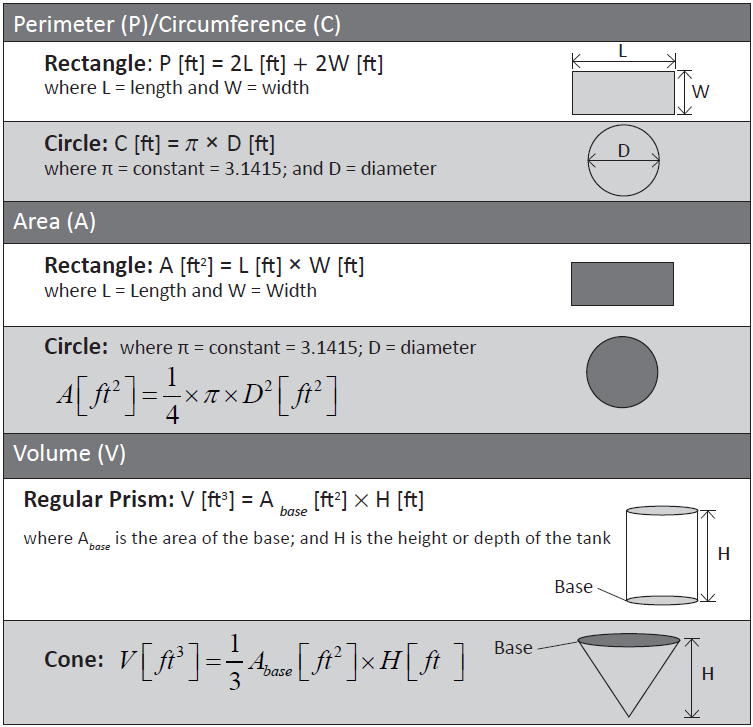
\includegraphics[scale=0.5]{Area&VolumeFormula}
\end{center}
\subsection{Example Problems}
% \hl{Example Problems}\\
\begin{enumerate}

\item The floor of a rectangular building is 20 feet long by 12 feet wide and the inside walls are 10 feet high. Find the total surface area of the inside walls of this building\\
Solution:\\
% \begin{center}
\begin{tikzpicture}
	%%% Edit the following coordinate to change the shape of your
	%%% cuboid
      
	%% Vanishing points for perspective handling
	\coordinate (P1) at (-7cm,1.5cm); % left vanishing point (To pick)
	\coordinate (P2) at (8cm,1.5cm); % right vanishing point (To pick)

	%% (A1) and (A2) defines the 2 central points of the cuboid
	\coordinate (A1) at (0em,0cm); % central top point (To pick)
	\coordinate (A2) at (0em,-2cm); % central bottom point (To pick)

	%% (A3) to (A8) are computed given a unique parameter (or 2) .8
	% You can vary .8 from 0 to 1 to change perspective on left side
	\coordinate (A3) at ($(P1)!.8!(A2)$); % To pick for perspective 
	\coordinate (A4) at ($(P1)!.8!(A1)$);

	% You can vary .8 from 0 to 1 to change perspective on right side
	\coordinate (A7) at ($(P2)!.7!(A2)$);
	\coordinate (A8) at ($(P2)!.7!(A1)$);

	%% Automatically compute the last 2 points with intersections
	\coordinate (A5) at
	  (intersection cs: first line={(A8) -- (P1)},
			    second line={(A4) -- (P2)});
	\coordinate (A6) at
	  (intersection cs: first line={(A7) -- (P1)}, 
			    second line={(A3) -- (P2)});

	%%% Depending of what you want to display, you can comment/edit
	%%% the following lines

	%% Possibly draw back faces

	\fill[gray!40] (A2) -- (A3) -- (A6) -- (A7) -- cycle; % face 6
	\node at (barycentric cs:A2=1,A3=1,A6=1,A7=1) {\tiny Floor=W*L};
	
	\fill[gray!50] (A3) -- (A4) -- (A5) -- (A6) -- cycle; % face 3
	\node at (barycentric cs:A3=1,A4=1,A5=1,A6=1) {\tiny Wall - W*H};
	
	\fill[gray!10, opacity=0.2] (A5) -- (A6) -- (A7) -- (A8) -- cycle; % face 4
	\node at (barycentric cs:A5=1,A6=1,A7=1,A8=1) {\tiny Wall - L*H};
	
	\fill[gray!10,opacity=0.5] (A1) -- (A2) -- (A3) -- (A4) -- cycle; % f2
	\node at (barycentric cs:A1=1,A2=1,A3=1,A4=1) {\tiny Wall - L*H};
	
	\fill[gray!40,opacity=0.2] (A1) -- (A4) -- (A5) -- (A8) -- cycle; % f5
	\node at (barycentric cs:A1=1,A4=1,A5=1,A8=1) {\tiny Ceiling=W*L};	
	
	\draw[thick,dashed] (A5) -- (A6);
	\draw[thick,dashed] (A3) -- (A6);
	\draw[thick,dashed] (A7) -- (A6);

	%% Possibly draw front faces

	%\fill[orange] (A1) -- (A8) -- (A7) -- (A2) -- cycle; % face 1
	\node at (barycentric cs:A1=1,A8=1,A7=1,A2=1) {\tiny Wall - W*H};
	


	%% Possibly draw front lines
	\draw[thick] (A1) -- (A2);

	\draw[<->] (-1.8,0.38) -- (-1.8,-1.3)node [midway, above=-1.8mm] {\hspace{-1.3cm}\tiny Height=10'};
	\draw[<->] (-1.6,-1.4) -- (-.3,-2.1)node [midway, above=-2.6mm] {\hspace{-1.3cm}\tiny Length=20'};
	\draw[<->] (2.6,-1.13) -- (0.2,-2.2)node [midway, below=.6mm] {\hspace{1.2cm}\tiny Width=12'};
	\draw[thick] (A3) -- (A4);
	\draw[thick] (A7) -- (A8);
	\draw[thick] (A1) -- (A4);
	\draw[thick] (A1) -- (A8);
	\draw[thick] (A2) -- (A3);
	\draw[thick] (A2) -- (A7);
	\draw[thick] (A4) -- (A5);
	\draw[thick] (A8) -- (A5);
	
	% Possibly draw points
	% (it can help you understand the cuboid structure)
%	\foreach \i in {1,2,...,8}
%	{
%	  \draw[fill=black] (A\i) circle (0.15em)
%	    node[above right] {\tiny \i};
%	}
	% \draw[fill=black] (P1) circle (0.1em) node[below] {\tiny p1};
	% \draw[fill=black] (P2) circle (0.1em) node[below] {\tiny p2};
\end{tikzpicture}\\
% \end{center}
2 Walls W*H + 2 Walls L*H= $2*12*10ft^2 + 2*20*10ft^2$\\
$=240+400=\boxed{640ft^2}$

2 Walls W*H + 2 Walls L*H + Floor + Ceiling= $2*12*10ft^2 + 2*20*10ft^2 + 2*12*20ft^2$\\
$=240+400+480=\boxed{1,120ft^2}$
\end{enumerate}
\item Concentration\\

Concentration is typically expressed as mg/l which is the weight of the constituent (mg) in 1 l (liter) of solution (wastewater).  As 1 l of water weighs 1 million mg, a concentration of 1 mg/l implies 1 mg of constituent per 1 million mg of water or one part per million (ppm).   \textbf{Thus, mg/l and ppm are synonymous.}\\  
Sometimes the constituent concentration is expressed in terms of percentage.\\
\vspace{6pt}
For example:  sludge containing 5\% solids or a 12.5\% chlorine concentration solution.\\
\vspace{6pt}
As one liter of water weighs 1,000,000 mg, one percent of that weight is 10,000 mg.  So 1\% solids implies 10,000 mg of solids per liter or 10,000 mg/l or 10,000 ppm.\\
\vspace{6pt}
$1\% concentration = 10,000 \enspace ppm \enspace or \enspace\dfrac{mg}{l}$\\
\vspace{6pt}
$0.1\% concentration = 1,000 \enspace ppm \enspace or \enspace \dfrac{mg}{l}$\\
\vspace{6pt}
$0.01\% concentration = 100 \enspace ppm \enspace or \enspace \dfrac{mg}{l}$\\
\vspace{6pt}
$10\% concentration = 100,000 \enspace ppm \enspace or \enspace \dfrac{mg}{l}$\\
\vspace{6pt}
$5\% concentration = 50,000 \enspace ppm \enspace or \enspace \dfrac{mg}{l}$\\
\vspace{6pt}
$A \enspace  12.5\% \enspace bleach \enspace solution \enspace contains \enspace 12.5\% \enspace or \enspace 125,000 \enspace \dfrac{mg}{l} \enspace of \enspace \enspace active \enspace chlorine $

\item Process Removal Efficiency

% \section{Process Removal Efficiency}\index{Process Removal Efficiency}
% \begin{snugshade*}
% 	\item \noindent\textsc{Process Removal Efficiency}
% \end{snugshade*}
\begin{itemize}
\item Process removal rate or removal efficiency is the percentage of the inlet concentration removed.  
\item It is used for quantifying the pollutant removal during wastewater treatment and is established based upon the amount of a particular wastewater constituent entering and leaving a treatment process.

\item $Process \enspace Removal \enspace Rate \enspace (\%) = \dfrac{Pollutant \enspace  In-Pollutant\enspace  Out}{Pollutant \enspace In}*100$\\

\item If 10 units of a pollutant are entering a process and 8 units of pollutant are leaving (process removes 2 units), then the process removal rate for that pollutant is (10-8)/10*100=20\%.  In this example the process is 20\% efficient in removing that particular pollutant.

\item The amount of pollutant can be measured in terms of concentration (mg/l) or in terms of mass loading (lbs).  The pounds formula is used for calculating the mass loadings.  
\end{itemize}
The above example is for calculating the removal efficiency using the inlet and outlet concentrations or mass loading.\\
The methods below can be used for calculating either the inlet or outlet pollutant concentrations, if the removal efficiency and the corresponding inlet or outlet concentrations are given. 


\hl{Case 1:  Calculating outlet conc. (X) given the inlet conc. and removal efficiency (RE\%):}

\tikzstyle{block} = [rectangle, draw, fill=red!40, 
    text width=6em, text centered, rounded corners, minimum height=3em]
\tikzstyle{arrow} = [draw, -latex']
\begin{figure}[!h]
\centering
\begin{tikzpicture}[node distance =1.5cm, auto]
    \draw ++(0,0) node [block] (Process) {Process};
   \node[node distance=1.9in] (dummy_in) [left of=Process] {In};
   \node[node distance=1.9in] (dummy_out) [right of=Process] {Out};
	\node (Removal) [below of=Process, yshift=-0in] {${Removal \enspace Efficiency=RE\% \enspace (Given)}$};
    \path [arrow] (dummy_in)-- (Process)  node [above] {\hspace{-5.8cm}$A \enspace mg/l \enspace (Given) $} node [below] {\hspace{-5.8cm}$100 \enspace mg/l$};
    \path [arrow] (Process) -- (dummy_out)  node [above] {\hspace{-4cm}$X \enspace mg/l \enspace (Unknown)$} node [below] {\hspace{-3.9cm}($100-RE\%)\enspace mg/l$};
   \draw[arrow] (Process) -- (Removal);
\end{tikzpicture}
\end{figure}
Using the fact that if the inlet concentration was 100 mg/l, the outlet concentration would be 100 minus the removal efficiency.\\
Setup the equation as:  $\dfrac{Out}{In}: \enspace \dfrac{X \enspace mg/l}{A \enspace mg/l}=\dfrac{100-RE\%}{100}$\\
Calculate X using cross multiplication - if $\dfrac{A}{B}=\dfrac{C}{D} \implies A=B*\dfrac{C}{D}$:\\
$X \enspace mg/l=A \enspace mg/l*\dfrac{100-RE\%}{100}$\\


\hl{Case 2:  Calculating inlet conc. (X) given the outlet conc. and removal efficiency (RE\%):}

\begin{figure}[!h]
\centering
\begin{tikzpicture}[node distance =1.5cm, auto]
    \draw ++(0,0) node [block] (Process) {Process};
   \node[node distance=1.9in] (dummy_in) [left of=Process] {In};
   \node[node distance=1.9in] (dummy_out) [right of=Process] {Out};
	\node (Removal) [below of=Process, yshift=-0in] {$Removal \enspace Efficiency=RE\% \enspace (Given)$};
    \path [arrow] (dummy_in)-- (Process)  node [above] {\hspace{-5.8cm}$X \enspace mg/l \enspace (Unknown)$} node [below] {\hspace{-5.8cm}$100 \enspace mg/l$};
    \path [arrow] (Process) -- (dummy_out)  node [above] {\hspace{-4cm}$A \enspace mg/l \enspace (Given)$} node [below] {\hspace{-3.9cm}($100-RE\%)\enspace mg/l$};
   \draw[arrow] (Process) -- (Removal);
\end{tikzpicture}
\end{figure}
Using the fact that if the inlet concentration was 100 mg/l, the outlet concentration would be 100 minus the removal efficiency.\\
Setup the equation as:  $\dfrac{In}{Out}: \enspace \dfrac{X \enspace mg/l}{A \enspace mg/l}=\dfrac{100}{100-RE\%}$\\
\vspace{0.3cm}
Calculate X using cross multiplication - if $\dfrac{A}{B}=\dfrac{C}{D} \implies A=B*\dfrac{C}{D}$:\\
$X \enspace mg/l=A \enspace mg/l*\dfrac{100}{100-RE\%}$\\

\vspace{0.4cm}
\subsection{Example Problems}
% \hl{Example Problems:}\\

\begin{enumerate}

\item What is the \% removal efficiency if the influent concentration is 10 mg/L and the effluent concentration is 2.5 mg/L?\\
$Removal \enspace Rate (\%) = \dfrac{In-Out}{In}*100 \implies \dfrac{10-2.5}{10}*100=\boxed{75\%}$



\item Calculate the outlet concentration if the inlet concentration is 80 mg/l and the process removal efficiency is 60\%\\
Solution:\\

\tikzstyle{block} = [rectangle, draw, fill=red!40, 
    text width=6em, text centered, rounded corners, minimum height=3em]
\tikzstyle{arrow} = [draw, -latex']
\begin{figure}[!h]
\centering
\begin{tikzpicture}[node distance =1.5cm, auto]
    \draw ++(0,0) node [block] (Process) {Process};
   \node[node distance=1.5in] (dummy_in) [left of=Process] {In};
   \node[node distance=1.5in] (dummy_out) [right of=Process] {Out};
	\node (Removal) [below of=Process, yshift=-0in] {$Removal \enspace Efficiency=60\%$};
    \path [arrow] (dummy_in)-- (Process)  node [above] {\hspace{-4.39cm}$80mg/l$} node [below] {\hspace{-4.39cm}$100mg/l$};
    \path [arrow] (Process) -- (dummy_out)  node [above] {\hspace{-3.cm}$Xmg/l$} node [below] {\hspace{-3cm}40mg/l};
   \draw[arrow] (Process) -- (Removal);
\end{tikzpicture}
%\caption[MFCC]{Diagrama en bloques del cálculo de las MFCC para un frame.}
%\label{MFCC}
\end{figure}

$\dfrac{Out}{In} \enspace:\enspace\dfrac{Actual \enspace Outlet (X)}{80}=\dfrac{100-60}{100}$\\
$\implies \dfrac{Actual \enspace Outlet (X)}{80} =0.4$\\
$\implies Actual \enspace  Outlet (X) = 0.4 * 80 = \boxed{32 mg/l}$\\


\item Calculate the inlet concentration if the outlet concentration is 80 mg/l and the process removal efficiency is 60\%\\

\tikzstyle{block} = [rectangle, draw, fill=red!40, 
    text width=6em, text centered, rounded corners, minimum height=3em]
\tikzstyle{arrow} = [draw, -latex']
\begin{figure}[!h]
\centering
\begin{tikzpicture}[node distance =1.5cm, auto]
    \draw ++(0,0) node [block] (Process) {Process};
   \node[node distance=1.5in] (dummy_in) [left of=Process] {In};
   \node[node distance=1.5in] (dummy_out) [right of=Process] {Out};
	\node (Removal) [below of=Process, yshift=-0in] {$Removal \enspace Efficiency=60\%$};
    \path [arrow] (dummy_in)-- (Process)  node [above] {\hspace{-4.39cm}$Xmg/l$} node [below] {\hspace{-4.39cm}$100mg/l$};
    \path [arrow] (Process) -- (dummy_out)  node [above] {\hspace{-3.cm}80mg/l} node [below] {\hspace{-3cm}40mg/l};
   \draw[arrow] (Process) -- (Removal);
\end{tikzpicture}
\end{figure}

$\dfrac{In}{Out} \enspace : \enspace \dfrac{Actual \enspace inlet \enspace  (X)}{80}=\dfrac{100}{100-60}\implies \dfrac{Actual \enspace inlet \enspace  (X)}{80}=2.5$\\    
Rearranging the equation:   $Actual \enspace inlet (X)=2.5*80 = \boxed{200 mg/l}$\\

\item If a plant removes 35\% of the influent BOD in the primary treatment and 85\% of the remaining BOD in the secondary system, what is the BOD of the raw wastewater if the BOD of the final effluent is 20mg/l\\
Solution:\\

\begin{figure}[!h]
\centering
\begin{tikzpicture}[node distance =1.5cm, auto]
    \draw ++(0,0) node [block] (Primary) {Primary};
    
   \node[node distance=1.9in] (dummy_in) [left of=Primary] {Influent BOD};
   \node[node distance=1.9in] (dummy_out) [right of=Primary] {Primary BOD Out};
	\node (Removal) [below of=Primary, yshift=-0in] {$Removal \enspace Efficiency=35\% $};
    \path [arrow] (dummy_in)-- (Primary)  node [above] {\hspace{-4.8cm}$X \enspace mg/l \enspace$} node [below] {};
    \path [arrow] (Primary) -- (dummy_out)  node [above] {\hspace{-4.9cm}$0.65X \enspace mg/l$} node [below] {};
   \draw[arrow] (Process) -- (Removal);
\end{tikzpicture}
\end{figure}


\begin{figure}[!h]
\centering
\begin{tikzpicture}[node distance =1.5cm, auto]
    \draw ++(0,0) node [block] (Secondary) {Secondary};
    
   \node[node distance=1.9in] (dummy_in) [left of=Secondary] {Primary BOD Out};
   \node[node distance=1.9in] (dummy_out) [right of=Secondary] {Secondary BOD Out};
	\node (Removal) [below of=Secondary, yshift=-0in] {$Removal \enspace Efficiency=85\% $};
    \path [arrow] (dummy_in)-- (Secondary)  node [above] {\hspace{-4.8cm}$0.65X \enspace mg/l \enspace$} node [below] {\hspace{-5cm}$100 \enspace mg/l$};
    \path [arrow] (Secondary) -- (dummy_out)  node [above] {\hspace{-4.9cm}$20 \enspace mg/l$} node [below] {\hspace{-4.9cm}$15 \enspace mg/l$};
   \draw[arrow] (Process) -- (Removal);
\end{tikzpicture}
\end{figure}
\vspace{0.3cm}
For the Secondary process:\\
$\dfrac{In}{Out}: \enspace \dfrac{0.65X}{20}=\dfrac{100}{15} \implies X \enspace mg/l=\dfrac{100*20}{15*0.65}=\boxed{205 \enspace mg/l}$\\

\vspace{0.3cm}
Alternate Solution \#1

$\xrightarrow[
				\text{X}\dfrac{mg}{l}
			]
			{
			\text{Influent BOD}
			}
 \boxed{Primary}
 \xrightarrow[
 				\text{X-0.35X=X*(1-0.35)=0.65X}\dfrac{mg}{l}
 			]
 			{
 			\text{Primary Effluent BOD}
 			}
 \boxed{Secondary}
 \xrightarrow[
				\text{0.65X-0.5525X=(0.65-0.5525)X=0.0975X }
			 ]
			{
			\text{Secondary Effluent BOD}
			}
$\\
\hspace{2.8cm}$\downarrow$ {\tiny(0.35X)BOD Removed}\hspace{3.2cm}$\downarrow$ {\tiny(0.65*0.85)X = 0.5525X BOD Removed}\\
$\implies 0.0975X=20 \implies X=\dfrac{20}{0.0975}=\boxed{205\dfrac{mg}{l}}$\\

\vspace{0.3cm}

Alternate Solution \#2:\\
$\xrightarrow[\text{X}\dfrac{mg}{l}]{\text{Influent BOD}}\boxed{Primary}\xrightarrow[\text{0.65X}]{\text{Primary Effluent BOD}}\boxed{Secondary}\xrightarrow[\text{(0.65*0.15)X}]{\text{Secondary Effluent BOD}}$\\
\hspace{2.8cm}$\downarrow$ {\tiny(0.35X)BOD Removed}\hspace{2.2cm}$\downarrow$ {\tiny(0.65X*0.85)BOD Removed}\\

Primary Effluent BOD = Influent BOD * (1-Primary BOD Removal), and\\
Secondary Effluent BOD=[Primary Effluent BOD]*(1-Secondary BOD Removal)\\
Secondary Eff. BOD=[Influent BOD * (1-Primary BOD Removal)]*(1-Secondary BOD Removal)\\

Therefore, 20 = [X*(1-0.35)] * (1-0.85)= X*0.65*0.15\\
$\implies 20 \enspace \dfrac{mg}{l}= 0.0975X \implies X=\dfrac{20}{0.0975}=\boxed{205 \enspace \dfrac{mg}{l}}$

\end{enumerate}
\item Pumping
% \section{Pumping}\index{Pumping}
% \pagebreak
% \begin{snugshade*}
% 	\item \noindent\textsc{Pumping}
% \end{snugshade*}
For Grades I \& II, pumping rate problems include the following:
% \begin{enumerate}
% \definecolor{shadecolor}{RGB}{225, 235, 235}
% \begin{snugshade*}
% \item \noindent\textsc{Calculating volume pumped in a given time interval given the pump flow rate\\}


\textbf{Method:\\}
\hspace{1cm}Step 1. Multiply the pump flow rate by the time interval\\
\textbf{Make sure:}
\begin{itemize}
\item The time units - in the given time interval and in the pump flow rate match
\end{itemize}
\subsection{Calculating time to pump a certain volume}\index{Calculating time to pump a certain volume}
% \begin{snugshade*}
% \item \noindent\textsc{Calculating time to pump a certain volume given the pump flow rate\\}
% \end{snugshade*}
\textbf{Method:}
\hspace{1cm}Step 1. Calculate the total volume pumped\\
\hspace{1cm}Step 2.	Divide the total volume by the pump flow rate\\
\textbf{Make sure:}
\begin{itemize}
\item The volume units - in the volume that needs to be pumped and in the pump flow rate match
\item The time unit in the pump flow rate needs to be converted to the time unit that you need the answer in
\end{itemize}
% \end{enumerate}


% \hl{Example Problems:}\\

\begin{enumerate}

\item A sludge pump is set to pump 5 minutes each hour. It pumps at the rate of 35 gpm. How many gallons of sludge are pumped each day?\\
Solution:\\
$\dfrac{35 \enspace gal \enspace sludge}{\cancel{min}}*\dfrac{5 \enspace \cancel{min}}{\cancel{hr}} *\dfrac{24 \enspace \cancel{hr}}{day}=\boxed{\dfrac{4,200 \enspace gallons}{day}}$\\
\vspace{0.5cm}

\item A sludge pump operates 5 minutes each 15 minute interval.  If the pump capacity is 60 gpm, how many gallons of sludge are pumped daily?

$\dfrac{60 \enspace gal \enspace sludge}{\xcancel{min}}*\dfrac{5 \enspace \xcancel{min}}{15 \enspace \cancel{min}}*1440\dfrac{\cancel{min}}{day}=\boxed{\dfrac {28,800 \enspace gal \enspace sludge }{day}}$\\

\item Given the tank is 10ft wide, 12 ft long and 18 ft deep tank including 2 ft of freeboard when filled to capacity. How much time (minutes) will be required to pump down this tank to a depth of 2 ft when the tank is at maximum capacity using a 600 GPM pump\\
Solution:\\
\vspace{0.5cm}


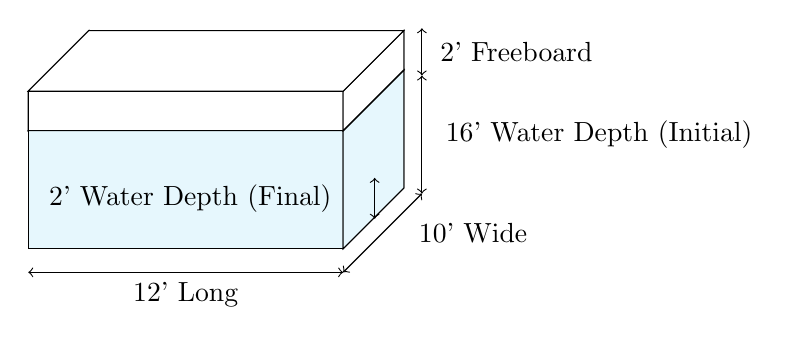
\begin{tikzpicture}

\pgfmathsetmacro{\cubexx}{4}
\pgfmathsetmacro{\cubeyy}{1.5}
\pgfmathsetmacro{\cubezz}{2}
\pgfmathsetmacro{\cubex}{4}
\pgfmathsetmacro{\cubey}{0.5}
\pgfmathsetmacro{\cubez}{2}
\pgfmathsetmacro{\cubexxx}{4}
\pgfmathsetmacro{\cubeyyy}{4}
\filldraw [fill=cyan!10!white, draw=black] (0,-\cubey,0) -- ++(-\cubexx,0,0) -- ++(0,-\cubeyy,0) -- ++(\cubexx,0,0) -- cycle ;
\filldraw [fill=cyan!0!white, draw=black] (0,-\cubey,0) -- ++(0,0,-\cubezz) -- ++(0,-\cubeyy,0) -- ++(0,0,\cubezz) -- cycle;
\filldraw [fill=cyan!10!white, draw=black] (0,-\cubey,0) -- ++(0,0,-\cubezz) -- ++(0,-\cubeyy,0) -- ++(0,0,\cubezz) -- cycle;
%\filldraw [fill=cyan!10!white, draw=black] (0,-\cubey,0) -- ++(-\cubexx,0,0) -- ++(0,0,-\cubezz) -- ++(\cubexx,0,0) -- cycle;
%%%\draw (0,-0.5,0) -- ++(-\cubex,0,0) -- ++(0,-\cubey,-\cubez) -- ++(\cubex,0,0) -- cycle;
\draw (-\cubex,0,0) -- ++(0,0,-\cubez) -- ++(0,-\cubey,0) -- ++(0,0,\cubez) -- cycle;
\draw (0,-\cubey,0) -- ++(-\cubex,0,0) -- ++(0,0,-\cubez) -- ++(\cubex,0,0) -- cycle;
\filldraw [fill=white, draw=black] (0,0,0) -- ++(-\cubex,0,0) -- ++(0,-\cubey,0) -- ++(\cubex,0,0) -- cycle ;
\filldraw [fill=white, draw=black] (0,0,0) -- ++(0,0,-\cubez) -- ++(0,-\cubey,0) -- ++(0,0,\cubez) -- cycle;
\filldraw [fill=white, draw=black] (0,0,0) -- ++(0,0,-\cubez) -- ++(0,-\cubey,0) -- ++(0,0,\cubez) -- cycle;
\filldraw [fill=white, draw=black] (0,0,0) -- ++(-\cubex,0,0) -- ++(0,0,-\cubez) -- ++(\cubex,0,0) -- cycle;

%\filldraw [fill=RoyalBlue!10!white, draw=black] (0,-1.5,0) -- ++(-\cubex,0,0) -- ++(0,-\cubey,0) -- ++(\cubex,0,0) -- cycle ;

%\filldraw [fill=RoyalBlue!10!white, draw=black] (0,-1.5,0) -- ++(0,0,-\cubez) -- ++(0,-\cubey,0) -- ++(0,0,\cubez) -- cycle;



%%\draw (0,-0.5,0) -- ++(-\cubex,0,0) -- ++(0,0,-\cubez) -- ++(\cubex,0,0) -- cycle;
%%\filldraw [fill=white, draw=black] (-\cubex,0,0) -- ++(0,0,-\cubez) -- ++(0,-\cubey,0) -- ++(0,0,\cubez) -- cycle;
%%\filldraw [fill=white, draw=black] (0,-\cubey,0) -- ++(-\cubex,0,0) -- ++(0,0,-\cubez) -- ++(\cubex,0,0) -- cycle ;

\draw [<->] (-4,-2.3) -- (0,-2.3) node [midway, below] {12' Long};
\draw [<->] (1,-1.3) -- (1,.2) node [midway, midway] {\hspace{4.5cm}16' Water Depth (Initial)};
\draw [<->] (0.4,-1.62) -- (0.4,-1.1) node [midway, midway] {\hspace{-4.8cm} 2' Water Depth (Final)};
\draw [<->] (1,.8) -- (1,.2) node [midway, midway] {\hspace{2.4cm}2' Freeboard};
\draw [<->] (1,-1.3) -- (0,-2.3) node [midway, midway] {\hspace{2.3cm}10' Wide};
\end{tikzpicture}\\
Volume to be pumped=$12 \enspace ft*10 \enspace ft *(16-2)\enspace ft=1,680ft^3$\\
\vspace{0.3cm}
$\implies \dfrac{1,680\cancel{ft^3}*7.48\dfrac{\cancel{gal}}{\cancel{ft^3}}}{600\dfrac{\cancel{gal}}{min}}=\boxed{21min}$
\end{enumerate}
\end{enumerate}

hydraulic grade line (HGL)\\
The surface or profile of water flowing in an open channel or a pipe flowing partially full. If a pipe is under pressure, the hydraulic grade line is that level water would rise to in a small, vertical tube connected to the pipe.\\

PRESSURE\\
Water pressure is measured in terms of pounds per square inch (psi) and feet of head (height of a water column in feet). A column of water 2.31 feet high creates a pressure of 1 psi. The water pressure at the bottom of a storagetank can be used to determine the water level in the tank.  Centrifugal pumps are rated in feet of Total Dynamic Head (TDH) but system pressures are measured in psi. All watersystem operators must be able to convert from one pressure unit to the other. .If the pressure (psi) is known, the height of the water column can be determined by multiplying the psi by 2.31.\\
$psi * 2.31 = Feet \enspace of \enspace Head$\\
EXAMPLE:\\
A pressure gauge at the bottom of a storage tank reads 30 psi. What is the water level in the tank?\\
Convert psi to feet of head\\
$30 psi * 2.31 = 69.3 \enspace feet \enspace of \enspace water \enspace above \enspace the \enspace gauge$\\
If the height of a column of water is known, the pressure it exerts can be determined by dividing the feet of head by 2.31.\\
$\dfrac{Head \enspace ft}{2.31} = psi$\\

EXAMPLE:\\
The reservoir level is 115 feet above the pump discharge. What is the discharge pressure on the pump?\\
Convert feet of head to psi.\\
$\dfrac{115 feet}{2.31} = 49.8 psi$\\


FLOW\\
The amount of water moving through the system can be measured in one of three different units. They are gpm (gallons per minute), mgd (millions of gallons per day), and cfs (cubic feet per second). The conversions are listed below.\\
$mgd x 700 = gpm $\\
$\dfrac{gpm}{700} = mgd$\\
$cfs x 449 = gpm $\\
$\dfrac{gpm }{449}= cfs$\\
EXAMPLES:\\
A system uses 2 mgd. How many gallons per minute does it use?\\
Convert mgd to gpm\\
$2 mgd x 700 = 1400 gpm$\\
A pipeline has a carrying capacity of 3 cfs. How many gpm can it handle?\\
Convert cfs to gpm\\
$3 cfs x 449 = 1347 gpm$\\
A well pumps 350 gpm. How many mgd will it pump?\\
Convert gpm to mgd\\
$\dfrac{350 gpm}{700} = 0.5 mgd$\\

AREAS\\
In order to calculate volumes of circular tanks and velocities in pipes, the area of the circle must first be determined. There are two basic formulae used to calculate the area of a circle.\\
$Area = 3.1416 x r2 Area = d2 x 0.785$\\
r = radius d = diameter\\
EXAMPLES:\\
A sedimentation basin is 60 feet in diameter. What is the surface area of the tank?\\
Calculate the area\\
$3.1416 x 30' x 30' = 2830 square feet$\\
$60' x 60' x 0.785 = 2830 square feet$\\
A pipeline has diameter of 12 inches. What is the area of the pipe?\\
Calculate the area\\
$3.1416 x 6" x 6" = 113 square inches$\\
$12" x 12" x 0.785 = 113 square inches$\\
VOLUMES\\
The volume of a rectangular tank can be determined by\\
multiplying the length, height, and width together.\\
Volume of rectangular tank (ft3) = L’ x H’ x W’\\
EXAMPLE:\\
A sedimentation basin is 60' long by 40' wide and 10'\\
deep. What is the volume of the tank in cubic feet?\\
Calculate the volume\\
60' x 40' x10' = 24,000 cubic feet (ft3)\\
The volume of a circular tank can be determined by multiplying the area of the by the height (or depth) of the tank. \\
$Volume of circular tank (ft3) = 3.1416 x r’2 x H’$\\
or\\
$Volume of circular tank (ft3) = d’2 x 0.785 x H’$\\
EXAMPLE:\\
A sedimentation basin is 60’in diameter and 12' deep. What is the volume of the tank?\\
Calculate the volume\\
$3.1416 x 30' x 30' x 12' = 33,900 cubic feet (ft3)$\\
or\\
$60' x 60' x 0.785 x 12' = 33,900 cubic feet (ft3)$\\
VOLUMES IN GALLONS\\
It is often necessary to calculate a volume of a tank or pipe in gallons rather than cubic feet. In most cases the volume must be calculated in cubic feet and then converted into gallons. This is determined by multiplying cubic feet by 7.48.\\
$Cubic feet x 7.48 = gallons$\\
EXAMPLE:\\
A sedimentation basin is 60' long by 40' wide and 10' deep. What is the volume of the tank in cubic feet?\\
Calculate the volume\\
$60' x 40' x10' = 24,000 ft3$\\
Convert cubic feet to gallons\\
$24,000 ft3 x 7.48 = 179,500 gallons$\\
A circular tank has a diameter of 40 feet and is 10 feet deep. How many gallons will it hold?\\
Calculate the volume\\
$1416 x 20' x 20' x 10' = 12,600 ft$3\\
or\\
$40' x 40' x 0.785 x 10' = 12,600 ft$3\\
Convert cubic feet to gallons\\
$12,600 ft3 x 7.48 = 94,200 gallons$\\
VOLUMES OF PIPES\\
The number of gallons contained in a one-foot section of pipe can be determined by squaring the diameter (in inches) and then multiplying by 0.0408. To determine the number of gallons in a particular length of pipe multiply the gallons per foot by the number of feet of pipe.\\
$Volume (gal) = D”2x 0.0408 x Length’$\\
EXAMPLES:\\
A 12" line is 1100 ft long. How many gallons does the pipe hold?\\
Find the volume of the pipe in gallons\\
$12" x 12" x 0.0408 x 1100 = 6460 gallons$\\
A 6" line is 654 ft long. How many gallons does the pipe hold?\\
Find the volume of the pipe in gallons\\
$6" x 6" x 0.0408 x 654 = 960 gallons$\\
VELOCITY\\
The velocity of the water moving through a pipe can be determined if the flow in cubic feet per second (cfs) and the diameter of the pipe (inches) are known. The area of the pipe must be calculated in square feet (ft2) and the flow is then divided by the area.\\
$\dfrac{Velocity (fps)}{ Area (ft2)} = Flow (cfs)$\\
EXAMPLE:\\
A 24" pipe carries a flow of 11 cfs. What is the velocity in the pipe? Change diameter in inches to feet\\
$24"/12" per ft = 2 ft.$\\
Find area of the pipe in sq.ft.\\
$1 x 1 x 3.1416 = 3.14 sq.ft$.\\
Find the velocity in fps\\
$\dfrac{11 cfs}{3.14 sq.ft.} = 3.5 fps$\\
The flow through a pipe (cfs) can be determined if the velocity and pipe diameter are known. The area of the pipe must be calculated in square feet and then multiplied by the velocity (fps.)\\
EXAMPLES:\\
A 12"’ pipe carries water at a velocity of 5.0 fps. What\\
is the flow in cfs?\\
Change inches to ft.\\
$12"/12" per ft = 1 ft.$\\
Find area of the pipe in sq.ft.\\
$0.5 x 0.5 x 3.1416 = 0.785 sq.ft.$\\
Find the flow in cfs\\
$5.0 fps x 0.785 sq.ft. = 3.9 cfs$\\
A 12" pipe carries 1400 gpm at 4.0 fps velocity and reduces to a 6" pipe. What is the velocity in the 6"\\
pipe?\\
Convert flow to cfs\\
$\dfrac{1400 gpm}{449 gpm/cfs}= 3.12 cfs$\\
Change inches to ft.\\
$\dfrac{6"}{12" per ft }= 0.5 ft$.\\
Find area of the pipe in sq.ft.\\
$0.25' x 0.25' x 3.1416 = 0.196 sq.ft.$\\
Find the velocity in fps\\
$3.12 cfs = 16 fps$\\
0.196 sq.ft.\\
DETENTION TIME\\
Detention time (D.T.) is the length of time in minutes or hours for one gallon of water to pass through a tank. To calculate detention time, the capacity of a tank in gallons is divided by the flow in gallons per minute (gpm) or gallons per day (gpd). If gpm is used, the answer will be in minutes and must be divided by 60 minutes to get hours. If gpd is used, the answer will be in days and must be multiplied by 24 hours. The detention time formula can also be used to calculate how long it will take to fill a tank.\\

EXAMPLES:\\
A 50,000 gallon tank receives 250,000 gpd flow. What is the detention time in hours?  Find detention time in days\\
$\dfrac{50,000 gal}{250,000 gal/day}. = 0.2 days$\\
Change days to hours\\
$0.2 days x 24 hrs/day = 4.8 hours$\\
A tank is 60' x 80' x 10' and the flow is 2.0 mgd? What is the detention time in hours? Find Volume in cubic feet\\
$60' x 80' X 10' = 48,000 cu.ft.$\\
Change cubic feet to gallons\\
$48,000 cu.ft. X 7.48 gal/cu.ft.= 359,000 gal$.\\
Change mgd to gal/day\\
$2.0 mgd = 2,000,000 gal/day$\\
Find D.T. in days\\
$\dfrac{359,000 gal}{2,000,000 gal/day} = 0.18 days$\\
Change days to hours\\
$0.18 days x 24 hrs/day = 4.3 hours$\\
A tank is 100' in diameter and 22 feet deep. If the flow into the tank is 1500 gpm and the flow out of the tank is 300 gpm, how many hours will it take to fill the tank?\\
Calculate the volume in cubic feet\\
$3.1416 x 50' x 50' x 22' = 173,000 ft3$\\
or\\
$100' x 100' x 0.785 x 22' = 173,000 ft3$\\
Change cubic feet to gallons\\
172,800 ft3 x 7.48 = 1,290,000 gallons\\
Calculate the net inflow\\
$1500 gpm – 300 gpm = 1200 gpm$\\
Calculate how long until full (detention time)\\
$\dfrac{1,290,000 gal}{1200 gpm} = 1075 minutes$\\
Change minutes to hours\\
$\dfrac{1075 min}{60 min/hr} = 17.9 hours$\\
DOSAGE\\
Chemical dosages are measured in ppm (parts per million) or mg/l (milligrams per liter.) Parts per million (ppm) is always a comparison of weight (pounds per million pounds). One pound of chemical added to one million pounds of water would be a dosage of 1 ppm. Since each gallon of water\\
weighs 8.34 pounds, one million gallons of water weighs 8.34 million pounds and would require 8.34 pounds of chemical to obtain a dosage of l ppm. Milligrams per liter (mg/l) is the metric term for a dosage equal to ppm. \\
$1 gallon = 8.34 lbs.$\\
$1 ppm = 1 mg/l$\\

The number of pounds of chemical needed to achieve a certain dosage can be determined by multiplying the ppm by the number of millions of gallons treated and then by 8.34 lbs/gal. The amount of water to be treated must always be in terms of millions of gallons (mgd). mg/l x mgd x 8.34 = pounds per day\\
EXAMPLE:\\
How many lbs/day of chlorine are needed to provide a dosage of 2.2 mg/l in 800,000 gal/day?\\
Change gal/day to mgd\\
$800,000 gpd = 0.8 mgd$\\
Calculate lbs/day\\
$2.2 mg/l x 0.8 mgd x 8.34 =14.7 lbs/day$\\
If HTH is used, instead of chlorine gas, only 65-70\% of each pound will be chlorine. Therefore, the amount of HTH must be calculated by dividing the pounds of chlorine needed by 0.65 or 0.70.\\
EXAMPLES:\\
A tank is 44' in diameter and 22' high and is dosed with 50 ppm of chlorine. How many pound of 70\% HTH is needed?\\
Find the volume of the tank in cubic feet\\
$22' x 22' x 3.1416 x 22' = 33,450 cu.ft.$\\
Change cu.ft. to gallons\\
$33,450 x 7.48 = 250,000 gallons$\\
Change gallons to mgd\\
$250,000 gallons = 0.250 mgd$\\
Find lbs of chlorine\\
$50 ppm x 0.25 mg x 8.34 = 104.25 lbs of chlorine$\\
Change percent available to a decimal equivalent\\
$70\% = 0.70$\\
Find lbs of HTH\\
$\dfrac{104.25 lbs Cl}{0.70}= 149 lbs of HTH$\\
A chlorine pump is feeding 10\% bleach at a dosage of 5 mg/l. If 2,200,000 gallons are treated in 16 hours, how many gallons per hour is the pump feeding?\\
Change gallons to mg\\
$2,200,000 gallons = 2.2 mg$\\
Find lbs of chlorine\\
$5 ppm x 2.2 mg x 8.34 = 91.7 lbs of Chlorine$\\
Change percent available to a decimal equivalent\\
$10\% = 0.10$\\
Find lbs of Bleach\\
$\dfrac{91.7 lbs Cl}{0.10}= 917 lbs of Bleach$\\
Find gallons of Bleach\\
$\dfrac{917 lbs Bleach}{8.34 lbs/gal} = 110 gallons of Bleach$\\

Find gallons per hour\\
110 gal. = 6.9 gal/hr\\
16 hr\\
A 12" pipe is 1880' long and must be disinfected with 50 ppm of 65\% HTH. How many pounds of HTH are needed? Find the volume of the pipe in gallons\\
$12" x 12" x .0408 x 1880' = 11, 045 gallons$\\
Change gallons to mgd\\
$11,045 gallons = 0.011 mgd$\\
Find lbs of chlorine\\
$50 ppm x 0.011 mgd x 8.34 = 4.6 lbs of Chlorine$\\
Change percent available to a decimal equivalent\\
$65\%= 0.65$\\
Find lbs of HTH\\
$4.6 lbs Cl = 7.1 lbs of HTH$\\
0.65\\
Liquid chemical dosages can be calculated to determine the gallons per day. Chemical feed pumps are calibrated using ml/min. If you take 3785 ml/gal and divide it by 1440 min/day, the conversion for gal/day to ml/min can be determined.\\
$\dfrac{3785 ml/gal}{1440 min/day} = 2.6 ml/min /gal/day$\\
Gal/day x 2.6 = ml/min\\
EXAMPLES:\\
A 20\% available Fluoride solution is used to dose 2,000,000 gpd at 450 ppb (parts per billion). How many ml/min is the pump feeding?\\
Change 450 ppb to ppm\\
$450 ppb = 0.45 ppm (mg/l)$\\
Change 2,000,000 gpd to mgd\\
$2,000,000 gpd = 2.0 mgd$\\
Find lbs of Fluoride\\
$0.45 ppm x 2.0 mgd x 8.34 = 7.5 lbs/day$\\
Change percent available to a decimal equivalent\\
$20\%= 0.2$\\
Find lbs of Fluoride solution\\
$7.5lbs F = 37.5 lbs of F solution$\\
0.2\\
Find gallons of fluoride\\
$37.5 lbs solution = 4.5 gpd$\\
8.34 lbs/gal\\
Change gallon/day to ml/min\\
$4.5 gpd x 2.6 = 11.7 ml/min$\\

An 18\% available Alum solution is used to dose 600,000 gpd at 25 mg/l. How many ml/min is the pump feeding?\\
Change 600,000 gpd to mgd\\
$25 mg/l x 0.6 mgd x 8.34 = 125 lbs/day$\\
Change percent available to a decimal equivalent 18\%= 0.18\\
Find lbs of Alum solution\\
$\dfrac{125 lbs Alum}{0.18} = 695 lbs of Alum solution$\\
Find gallons of Alum\\
$\dfrac{695 lbs solution}{8.34 lbs/gal} = 83.3 gpd$\\
Change gallon/day to ml/min\\
$83.3 gpd x 2.6 = 217 ml/min$\\
Sometimes there is too much information in the question.\\
The example below has too much information. The well\\
flow and storage tank data are not needed to work the\\
problem.\\
EXAMPLE:\\
A system has a well that produces 200 gpm and a 1500 gallon storage tank. There are 120 homes on the systems and the average daily consumption is 350 gallons/home. A chlorine dosage of 1.3 ppm is maintained using 65\% HTH. How many pounds of HTH must be purchased each year?\\
Find system consumption\\
$120 homes x 350 gallons/day/home = 42,000 gpd$\\
Change gallons/day to mgd\\
$42,000 gallons/day = 0.042 mgd$\\
Find lbs/day of chlorine\\
$1.3 ppm x 0.042 mg x 8.34 = 0.45 lbs/day of Cl$\\
Change percent available to a decimal equivalent\\
$65\% = 0.65$\\
Find lbs/day of HTH\\
$\dfrac{0.45 lbs Cl}{ 0.65}= 0.7 lbs/day of HTH$\\
Find lbs/year of HTH\\
$0.7 lbs/day x 365 days/year = 255.5 lbs/year$\\
WIRE-TO-WATER CALCULATIONS\\
The term wire-to-water refers to the conversion of electrical horsepower to water horsepower. The motor takes electrical energy and converts it into mechanical energy. The pump turns mechanical energy into hydraulic energy. The electrical energy is measured as motor horsepower (MHp.) The mechanical energy is measured as brake horsepower (BHp.) And the hydraulic energy is measured as water horsepower (WHp.)\\

Horsepower is measured by lifting a weight a given distance in a specific time period. One horsepower is the amount of energy required to produce 33,000 ft-lbs of work per minute. That means that lifting 33,000 pounds one foot in one minute or lifting one pound 33,000 feet in the air in one minute\\
would both require one horsepower worth of energy. When water is pumped, performance is measured in flow (gallons/minute) and pressure (feet of head). If you multiply gallons per minute and feet of head the resulting units would be gallon-feet per minute. Multiply gallon-feet per minute by 8.34 pounds/gallon and the units become foot pounds (of water) per minute. This can now be converted to water horsepower by dividing by 33,000 ft-lbs/min per horsepower.\\
$\dfrac{Gpm}{33,000 ft-lbs/min/Hp} x 8.34 x Feet of Head = Water Horsepower (WHp)$\\
This equation can be further simplified to:\\
$\dfrac{Gpm}{3960}x Feet of Head = Water Horsepower (WHp)$\\
Brake horsepower is the amount of energy that must go into the pump to produce the required WHp. Loses due to friction and heat in the pump reduce the pump’s efficiency and require more energy in than goes out. If a pump is 80\% efficient, it requires 10 BHp to generate 8 WHp.\\
$\dfrac{BrakeHp}{ Pump Efficiency}= WaterHp$\\
Motor horsepower is the amount of electrical energy that must go into the motor to produce the required BHp. Loses due to friction and heat in the motor reduce the motor’s efficiency and require more energy in than goes out. If a motor is 88\% efficient, it requires 10 BHp to generate 8.8 BHp.\\
$\dfrac{MotorHp}{ Motor Eff} = BrakeHp$\\
or\\
$\dfrac{MotorHp}{ Motor Eff x Pump Eff }= WaterHp$\\

Motor horsepower can be converted into kilowatts by multiplying by 0.746 Kw/Hp. Kilowatt-hours can be determined by multiplying kilowatts by run time in hours. MotorHp x 0.746 Kw/Hp x Hours = Kw-Hours of electricity The following example has seven problems that relate to wire-to-water calculations. Each problem will take the calculation one step further. It is intended to show how the steps are linked, not to represent an example of a set of exam questions. An actual exam question would possibly\\
require the calculation of Water horsepower (Problems 1-3) or calculation of cost of operation (Problems 1-7).\\
Pump Data:\\
6 Feet - Negative Suction Head\\
96 Feet - Discharge Head\\
17 Feet - Friction Loss\\
400 gpm - Flow\\
Motor Efficiency - 90\%\\
Pump Efficiency - 80\%\\
What is the static head on the pump?\\
$96 ft + 6 ft = 102 ft$\\
What is the total dynamic head?\\
$96 ft + 6 ft + 17 ft = 119 ft TDH$\\
What is the Water Horsepower that the pump delivers?\\
$\dfrac{400 gpm }{3960}x 119 ft = 12 WHp$\\
What is the Brake Horsepower?\\
Change 80\% to a decimal\\
Find Brake Horsepower\\
$\dfrac{12 Whp*0.80 Pump Eff} = 15 BHp$\\
What is the Motor Horsepower?\\
Change 90\% to a decimal\\
90\% = 0.90\\
Find Motor Horsepower\\
15 BHp = 16.7 MHp\\
0.90 Motor Eff\\
How many Kilowatts of electricity does the motor 
require?\\
6.7 MHp x 0.746 Kw/Hp = 12.5 Kw\\
If the pump runs 13 hours a day and electric rates are \$0.09/Kw-Hour; How much does it cost to run the pump for a month (30 days)?\\
Find Kw-Hours per day\\
$12.5 Kw x 13 hours/day = 162 Kw-Hours/day$\\
Find cost per day\\
$162 Kw-Hours x \$0.09/KwHour = \$14.58/day$\\
Find cost for the month\\
$14.58/day x 30 days/month = \$437.40/month$\\

\end{document}
%%
\part{Week 5}
\chapterimage{Water1.png} % Chapter heading image

\chapter{Water Treatment I}

Lorem ipsum dolor sit amet, consectetur adipiscing elit, sed do eiusmod tempor incididunt ut labore et dolore magna aliqua. Vitae et leo duis ut. Eget gravida cum sociis natoque. Fusce id velit ut tortor. Nibh venenatis cras sed felis eget velit. In mollis nunc sed id semper risus in hendrerit. Volutpat odio facilisis mauris sit. Enim diam vulputate ut pharetra. Viverra vitae congue eu consequat. Sapien faucibus et molestie ac. Quam pellentesque nec nam aliquam sem et. Sed elementum tempus egestas sed sed risus pretium quam. Vel pharetra vel turpis nunc eget lorem dolor sed viverra. Ornare aenean euismod elementum nisi quis eleifend. Eget arcu dictum varius duis.
%%
\part{Week 6}
\chapterimage{Water1.png} % Chapter heading image

\chapter{Water Treatment II}



Lorem ipsum dolor sit amet, consectetur adipiscing elit, sed do eiusmod tempor incididunt ut labore et dolore magna aliqua. Ornare quam viverra orci sagittis eu volutpat odio facilisis mauris. Amet massa vitae tortor condimentum lacinia quis vel eros donec. Integer eget aliquet nibh praesent tristique magna sit. Sit amet massa vitae tortor condimentum. Ut sem nulla pharetra diam sit amet. Mauris cursus mattis molestie a iaculis at erat. Pulvinar etiam non quam lacus suspendisse. Risus at ultrices mi tempus imperdiet nulla malesuada pellentesque elit. Viverra accumsan in nisl nisi scelerisque. Justo nec ultrices dui sapien. Nulla facilisi morbi tempus iaculis urna id volutpat lacus laoreet. Tortor posuere ac ut consequat semper viverra nam libero justo. Sit amet nisl suscipit adipiscing bibendum est ultricies integer. Eget gravida cum sociis natoque penatibus et magnis dis. Mi ipsum faucibus vitae aliquet nec ullamcorper sit amet risus. Sagittis nisl rhoncus mattis rhoncus urna neque viverra justo. Non tellus orci ac auctor augue mauris augue.

%%
%\part{Week 7}
%\chapterimage{Water1.png} % Chapter heading image

\chapter{Review}

Lorem ipsum dolor sit amet, consectetur adipiscing elit, sed do eiusmod tempor incididunt ut labore et dolore magna aliqua. Consequat semper viverra nam libero justo. Hendrerit gravida rutrum quisque non tellus orci ac auctor augue. Purus in mollis nunc sed id semper. Donec enim diam vulputate ut pharetra sit amet aliquam. Nibh venenatis cras sed felis eget. Aliquam id diam maecenas ultricies. Fringilla urna porttitor rhoncus dolor purus. Morbi non arcu risus quis varius quam quisque. Aliquet bibendum enim facilisis gravida neque convallis a cras semper. Semper quis lectus nulla at volutpat diam ut venenatis. Fames ac turpis egestas maecenas pharetra convallis posuere morbi. Egestas erat imperdiet sed euismod nisi porta lorem. Vitae sapien pellentesque habitant morbi tristique senectus.
%%
%\part{Module 9}
%\chapterimage{Dewatering.jpg} % Chapter heading image

\chapter{Solids Treatment}

\section{Why do we need to treat wastewater solids?}\index{Why do we need to treat wastewater solids?}

\begin{itemize}
\item Sludge is generated from the wastewater treatment processes -  settled solids and scum from primary and secondary treatment processes
\item This sludge contain organic compounds and also elements that are beneficial plant nutrients
\item However, the organic solids in the sludge are not stable (i.e. they will decay) and include pathogens.  \item Prior to disposal, sludge has to be treated – stabilized, so that its disposal or reuse does not pose a threat to public health.
\item Sludge treatment is very critical as it is an expensive process and sludge disposal is subject to strict regulatory requirement.
\item Even solids are only a small component of wastewater, the solids treatment and disposal account for a very substantial portion of wastewater treatment costs.  Typically 40 to 60\% of total wastewater treatment operations cost is attributable to sludge treatment and disposal.
\end{itemize}

\textbf{NOTE: Solids removed during Preliminary Treatment, from barscreens and grit chambers are typically not treated as part of the solids treatment process.  These solids are disposed off at a landfill}

\vspace{0.5cm}
\textbf{Typical solids treatment is comprised of the following three sequential steps:
\begin{enumerate}
\item Sludge thickening
\item Sludge stabilization
\item Sludge dewatering
\end{enumerate}}
\vspace{0.5cm}
\section{Sludge thickening}\index{Sludge thickening}
Sludge thickening involves the removal of excess water from the primary and secondary sludge increasing the solids content of the sludge and reducing the volume of sludge to be treated in the sludge stabilization process.
Sludge thickening reduces the volume of sludge that need to be handled in the sludge stabilization step thereby reducing treatment cost.  
\begin{itemize}
\item There is an upper limit of the solids concentration that can be effectively treated (stabilized) as increasing the solids concentration reduces its ability to be mixed and pumped easily.  Typically the sludge thickening process produces sludge with a solids content of less than 10\%.\\
\end{itemize}
Benefits of thickening to the sludge stabilization process include:
\begin{itemize}
\item Improved performance due to a lower volume of sludge
\item Cost savings in the construction of new facilities
\item Reduction in energy requirements as less water has to be heated
\end{itemize}
Typical methods used for sludge thickening include:
\begin{enumerate}
\item Gravity thickener - more suitable for primary sludge
\item Dissolved air floatation thickener - more suitable for lighter, fluffier floc such as the secondary sludge.
\end{enumerate}
\section{Sludge Stabilization}\index{Sludge Stabilization}
\textbf{}\\
Sludge stabilization process produces solids that are deemed safe for eventual disposal.  Federal Part 503 rule establishes requirements for the final use or disposal of sewage sludge.  The solids disposal methods may include: land application, as a crop/vegetation fertilizer, placed on a surface disposal site for final disposal and fired in an incinerator.\\
\textbf{Biosolids is the term used for stabilized sludge which meets regulatory standards for beneficial reuse}\\  

Sludge stabilization process results in the following:
\begin{enumerate}
\item Reduction in amount of solids
\item Pathogen reduction
\item Odor reduction
\item Reduction in vector attraction
\end{enumerate}
The main processes involved in sludge stabilization include:
\begin{itemize}
\item Digestion - Aerobic or anaerobic
\item Lime or alkaline stabilization
\item Composting
\item Long term storage in lagoons
\item Thermal processes
\item Incineration
\end{itemize}

Most common processes involved in sludge stabilization include:

		\begin{enumerate}
		\item Digestion - Aerobic or anaerobic
		\item Lime or alkaline stabilization
		\item Composting
		\item Long term storage in lagoons
		\item Thermal processes
		\item Incineration
		\end{enumerate}
		\begin{itemize}
		\item \hl{Sludge digestion is a microbiological process and is the most common sludge stabilization method}.
		\item There are two major sludge digestion processes:
			\begin{itemize}
			\item aerobic digestion which utilizes aerobic microorganisms, and produces carbon dioxide as a byproduct
			\item anaerobic digestion which utilizes anaerobic microorganisms and it produces digester gas as a byproduct.
			\item Digester gas is typically composed of 60-65\% methane gas with the remainder being mostly carbon dioxide ($CO_2$) and is useful because of its potential use as fuel - energy recovery from wastewater.
			\end{itemize}
		\end{itemize}

\subsection{Anaerobic Digestion Process Basics}\index{Anaerobic Digestion Process Basics}

		\begin{itemize}
		\item Solids removed from the primary and secondary treatment processes is fed to the digesters.  
		\item The sludge feed to the digesters range between 3 – 6\% total solids which typically contain 70\% organic solids
		\item The anaerobic digester is typically a large cylindrical concrete tank and is operated as a continuous process at a fixed volume\\ $\implies$ as sludge is fed into the digester it displaces an equal amount of sludge which leaves the digester.
\begin{center}
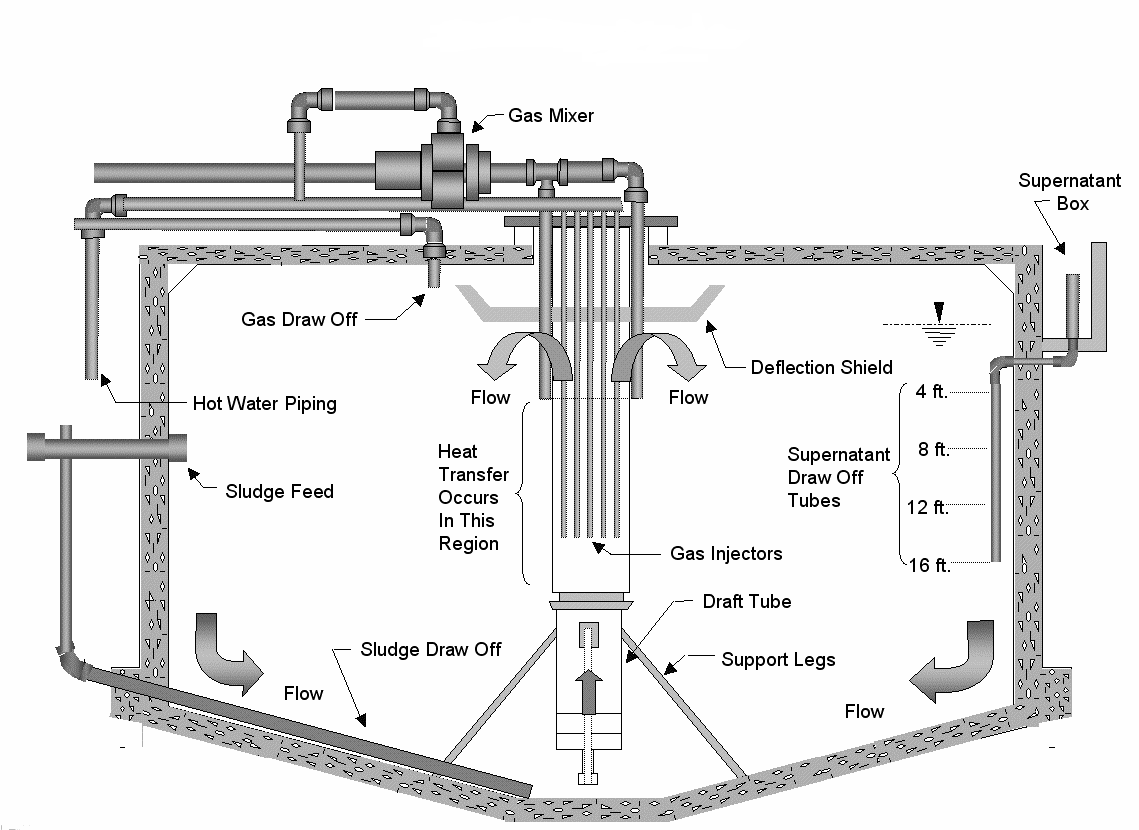
\includegraphics[scale=0.50]{DigesterFixedCover}\\
\textbf{Anaerobic Digester}\\
\end{center}
		\item The sludge typically occupies 70 - 90\% of the total digester volume and the methane carbon dioxide gas mixture occupies the headspace from where it is withdrawn also on a continuous basis.
		\item In the anaerobic digestion process microorganisms convert volatile matter into mainly methane (CH$_4$) and carbon dioxide (CO$_2$)
		\item The sludge content of the digesters is kept mixed and maintained in a constant temperature range using external heating.
		\item The activity and type of bacteria present in the digester is dictated by the operating temperature of the digester.
		\item Anaerobic digestion can be in the following three temperature ranges, each of which has its own unique microbiology.\\
			\begin{enumerate}[1. ]
			\item Psychrophilic digester:  Digester is maintained between 50  - 65 F.  Sludge detention time - 50 to 180 days
			\item Mesophilic digesters: – Digester is most commonly operated  between 95 – 98 F and the typical number of days required for digestion is between 15 to 30 days.\\
			\item Thermophilic digesters:  These digesters’ optimal operating temperatures range is between 113   135 F and it typically requires 5 to 12 days.\\
			\end{enumerate}     
		\item These organic solids are measured as volatile solids (VS).  
		\item The volatile solids content of the sludge entering and leaving the digester are measured to quantify the solids removal in the digester
		 \item Breakdown of volatile matter in the sludge ultimately into methane (CH$_4$) and carbon dioxide (CO$_2$) occurs in multiple steps involving different groups of microorganisms as follows:\\
			\begin{enumerate}[Step 1.]
			\item Hydrolysis:  Here the microorganisms breakdown complex organic matter in the sludge - carbohydrates, proteins, lignin, and lipids into simpler compounds including sugars, soluble fatty acids and amines.\\
			\item Acid Formation:  The simpler compounds formed in Step 1 are converted to organic acids by acid forming bacteria\\
			\item Methane Formation: The organic acids formed in Step 2 are converted into methane and carbon dioxide by methane forming bacteria.\\
			\end{enumerate}
		\item Gas production ranges between 10 to 16 cubic feet per pound of volatile matter destroyed and the gas production remains stable over time.
		\item Low gas production indicates problems - toxicity, temperature, volatile acid to alkalinity ratio, mixing, or feed rates.
		\end{itemize}


\section{Sludge Dewatering}\index{Sludge Dewatering}
Solids stabilized using digestion process has only a small percentage by weight of solids -less than 5\%.  It therefore becomes necessary to dewater the stabilized sludge prior to hauling off-site for final disposal.  Like thickening, the dewatering process does not treat the sludge.  It increases the solids content to between 15 to 30 percent and the higher solids content of the stabilized sludge makes it easier to handle and reduces costs associated with elements related to accomplishing the end objectives with the sludge – land application, composting, drying, incineration or landfill.\\
Dewatering involves conditioning the sludge with a polymer and subjecting it to a physical process which include:
\begin{enumerate}
\item Belt Filter Press 
\item Centrifuge
\end{enumerate}


%
%\part{Module 10}
%\chapterimage{FutureChapterImage2.png}
\chapter{Wastewater Treatment - Future}

\section{Water Resource Recovery Facility - WRRF}\index{Water Resource Recovery Facility - WRRF}
\begin{itemize}
\item Originally, the function of a wastewater treatment plant was collection, treatment and disposal which was driven solely by the need to reduce human disease and to protect the environment.
\item It was soon realized that wastewater contains valuable elements like organic matter, phosphorus, nitrogen, rare metals and thermal energy
\item The scope of wastewater treatment has now evolved to encompass recovering valuable resources contained in the wastewater.
\item The wastewater treatment plant is now known as a water resource recovery facility (WRRF). 
\item This change reflects the new focus on the products and benefits of treatment rather than its original and only objective - treating water for sanitation.
\item The WRRF is being adapted into the concept of the circular economy in which products, materials (and raw materials) remain in the economy for as long as possible, and waste is treated as secondary raw materials that can be recycled to process and re-used.  This distinguishes it from a linear economy which is based on the: "take-make-use-dispose" system, in which waste is usually the last stage of the product life cycle.

\end{itemize}

\subsection{Water}\index{Water}
\begin{itemize}
\item Municipal wastewater reuse offers the potential to significantly increase the nation’s total available water resources. Of the 32 billion gallons of treated wastewater discharged nationally, approximately 12 billion gallons of treated wastewater is discharged each day to an ocean or estuary.
\item WRRF is key to the use of treated wastewater, or “reclaimed” water, for beneficial purposes such as drinking, irrigation, or industrial uses—is one option that has helped some communities significantly expand their water supplies.
\item Wastewater can be treated to various qualities to satisfy demand from different sectors, including industry and agriculture. It can be used to maintain the environmental flow, or even reused as drinking water. 
\item Wastewater treatment is one solution to the water scarcity issue, and also to the problem of water security, freeing water resources for other uses or for preservation.
\end{itemize}




\subsection{Energy}\index{Energy}
\begin{itemize}
\item In the US, municipal wastewater treatment plants consume 30 terawatt-hours per year of electricity which is about 0.1\% of the total electrical consumption.  
\item WRRFs have the potential to be energy neutral or even net energy producers through comprehensive energy management approaches, incorporating efficient practices, and generating renewable energy from their by-products, such as biosolids.

\item By making the treatment processes more energy efficient and through the recovery of chemical or calorific energy in the wastewater play a key role in reducing the carbon foot print of the WRRF. 

\item Given the amount of chemical or calorific energy contained in wastewater, the goal is for the WRRFs to be energy neutral or even energy positive - which is to produce same or more energy than the energy needed for treatment.
\end{itemize}


\subsection{Nutrients}\index{Nutrients}
\begin{itemize}
\item Nutrient recovery is the practice of recovering nutrients such as nitrogen and phosphorus from used water streams that would otherwise be discarded/disposed and converting them into fertilizer used for ecological and agricultural purposes. 
\item Phosphate used in fertilizers is manufactured from phosphate rock using a very environmentally detrimental mining process.  Recovery/reuse of phosphate from wastewater mitigates dependence on this mined mineral.
\end{itemize} 
Nutrient recovery at a WRRF is accomplished using one of following two methods:
\begin{enumerate}[1.] 
\item By precipitating phosphorous as struvite crystals using a dedicated reactor. The struvite crystals are collected and resold as fertilizer which has a resale value ranging from \$100-\$600 per dry ton.  Benefits of this method include:
\begin{itemize}
\item Generation of revenue from the fertilizer produced
\item Reduces fouling of equipment due to precipitation of struvite formed during the solids treatment process
\item Allows for meeting NPDES nutrients discharge limits
\end{itemize}
\item Nutrient recovery can also be achieved through the land application of biosolids. Benefits of land application of biosolids include:
\begin{itemize}
\item Provide primary nutrients - nitrogen and phosphorous and secondary nutrients such as calcium, iron, magnesium and zinc for crops.
\item The organic carbon and organic matter in the biosolids help build better soils. 
\item Allows for sequestering carbon in the soil.
\end{itemize}
\end{enumerate}


\section{Challenges to WRRF}\index{Challenges to WRRF}

\subsection{Constituents of Emerging Concern}\index{Constituents of Emerging Concern}
\begin{itemize}
\item Constituents of Emerging Concern (CECs) include a variety of substances such as medicines, personal care products, flame retardants, algal toxins, micorplastics, and many others that are not currently federally regulated but known to occur in water.
\item Some of these CECs, incuding hormones, PFAS, and endocrine disruptors are known to pose health risks to humans and aquatic life.
\item Although some CECs that reach WRRFs are destroyed through wastewater treatment and solids processing, some recalcitrant microconstituents and their metabolites may pass through the treatment process intact and may end up in the effluent or biosolids. 
\item Both, the dose (concentration) of the CEC present and frequency/duration of exposure is important for interpreting possible risk to ecological and human health.
\item The CECs move in their complex cycling through surface and groundwaters across the planet - from potable water to wastewater and viceversa as potable water is converted into wastewater followed by uptake of the treated wastewater by the potable water supply system through groundwater contaminated by the percolation of these CECs in land applied wastewater biosolids or through the CECs in the treated wastewater discharge to surface water such as a lake or river.
\item The CECs concentrations in the plant influent range typically in nano-g/L to micro-g/L , in effluent from non-detect to nano-g/L, and in biosolids the concentrations vary from micro-g/kg to mg/kg.
\end{itemize}


\subsection{Decentralized and Distributed Systems}\index{Decentralized and Distributed Systems}
\begin{itemize}
\item To make the wastewater treatment systems more sustainable and to overcome the issues of a centralized system where wastewater is collected from various areas and cities in urban areas and conveyed to a centrally located plant for treatment, it is imperative to consider 
\item \textbf{Distributed systems} are in different geographical locations, but are linked to a central system either physically, or by management. \textbf{Decentralized systems} can be located in a different geographical location, but are not linked physically, or are not managed under the umbrella of a centralized system.
\item Through the selection of correct locations and appropriate technologies, distributed or decentralized systems can:
\begin{itemize}
\item Provide environmental benefits, such as nutrient and pathogen removal
\item Provide water for direct potable reuse and non-potable water in both rural and urban settings for purposes such as flushing, cooling and heating, landscaping, and subsurface irrigation drip.
\end{itemize}
\end{itemize}


\subsection{Climate Change}\index{Climate Change} 
\begin{itemize}
\item Climate change has directly impacted water resources by altering precipitation patterns, severe drought and floods, snowpack amount, elevation, stream flow, and rising sea levels. 
\item This has created a direct need for utilities to manage local water resources to lessen the potential impact of climate change. 
\item By increasing water reuse, developing resiliency and other actions, WRRFs can be a leader in fighting and preparing for climate change effects.
\item Driven largely by climate change factors, lower carbon footprint - the amount of carbon dioxide and other carbon compounds emitted due to the consumption of fossil fuels (energy), and lower energy demands are now being factored in when assessing wastewater treatment options.
\end{itemize}
\newpage
\begin{center}
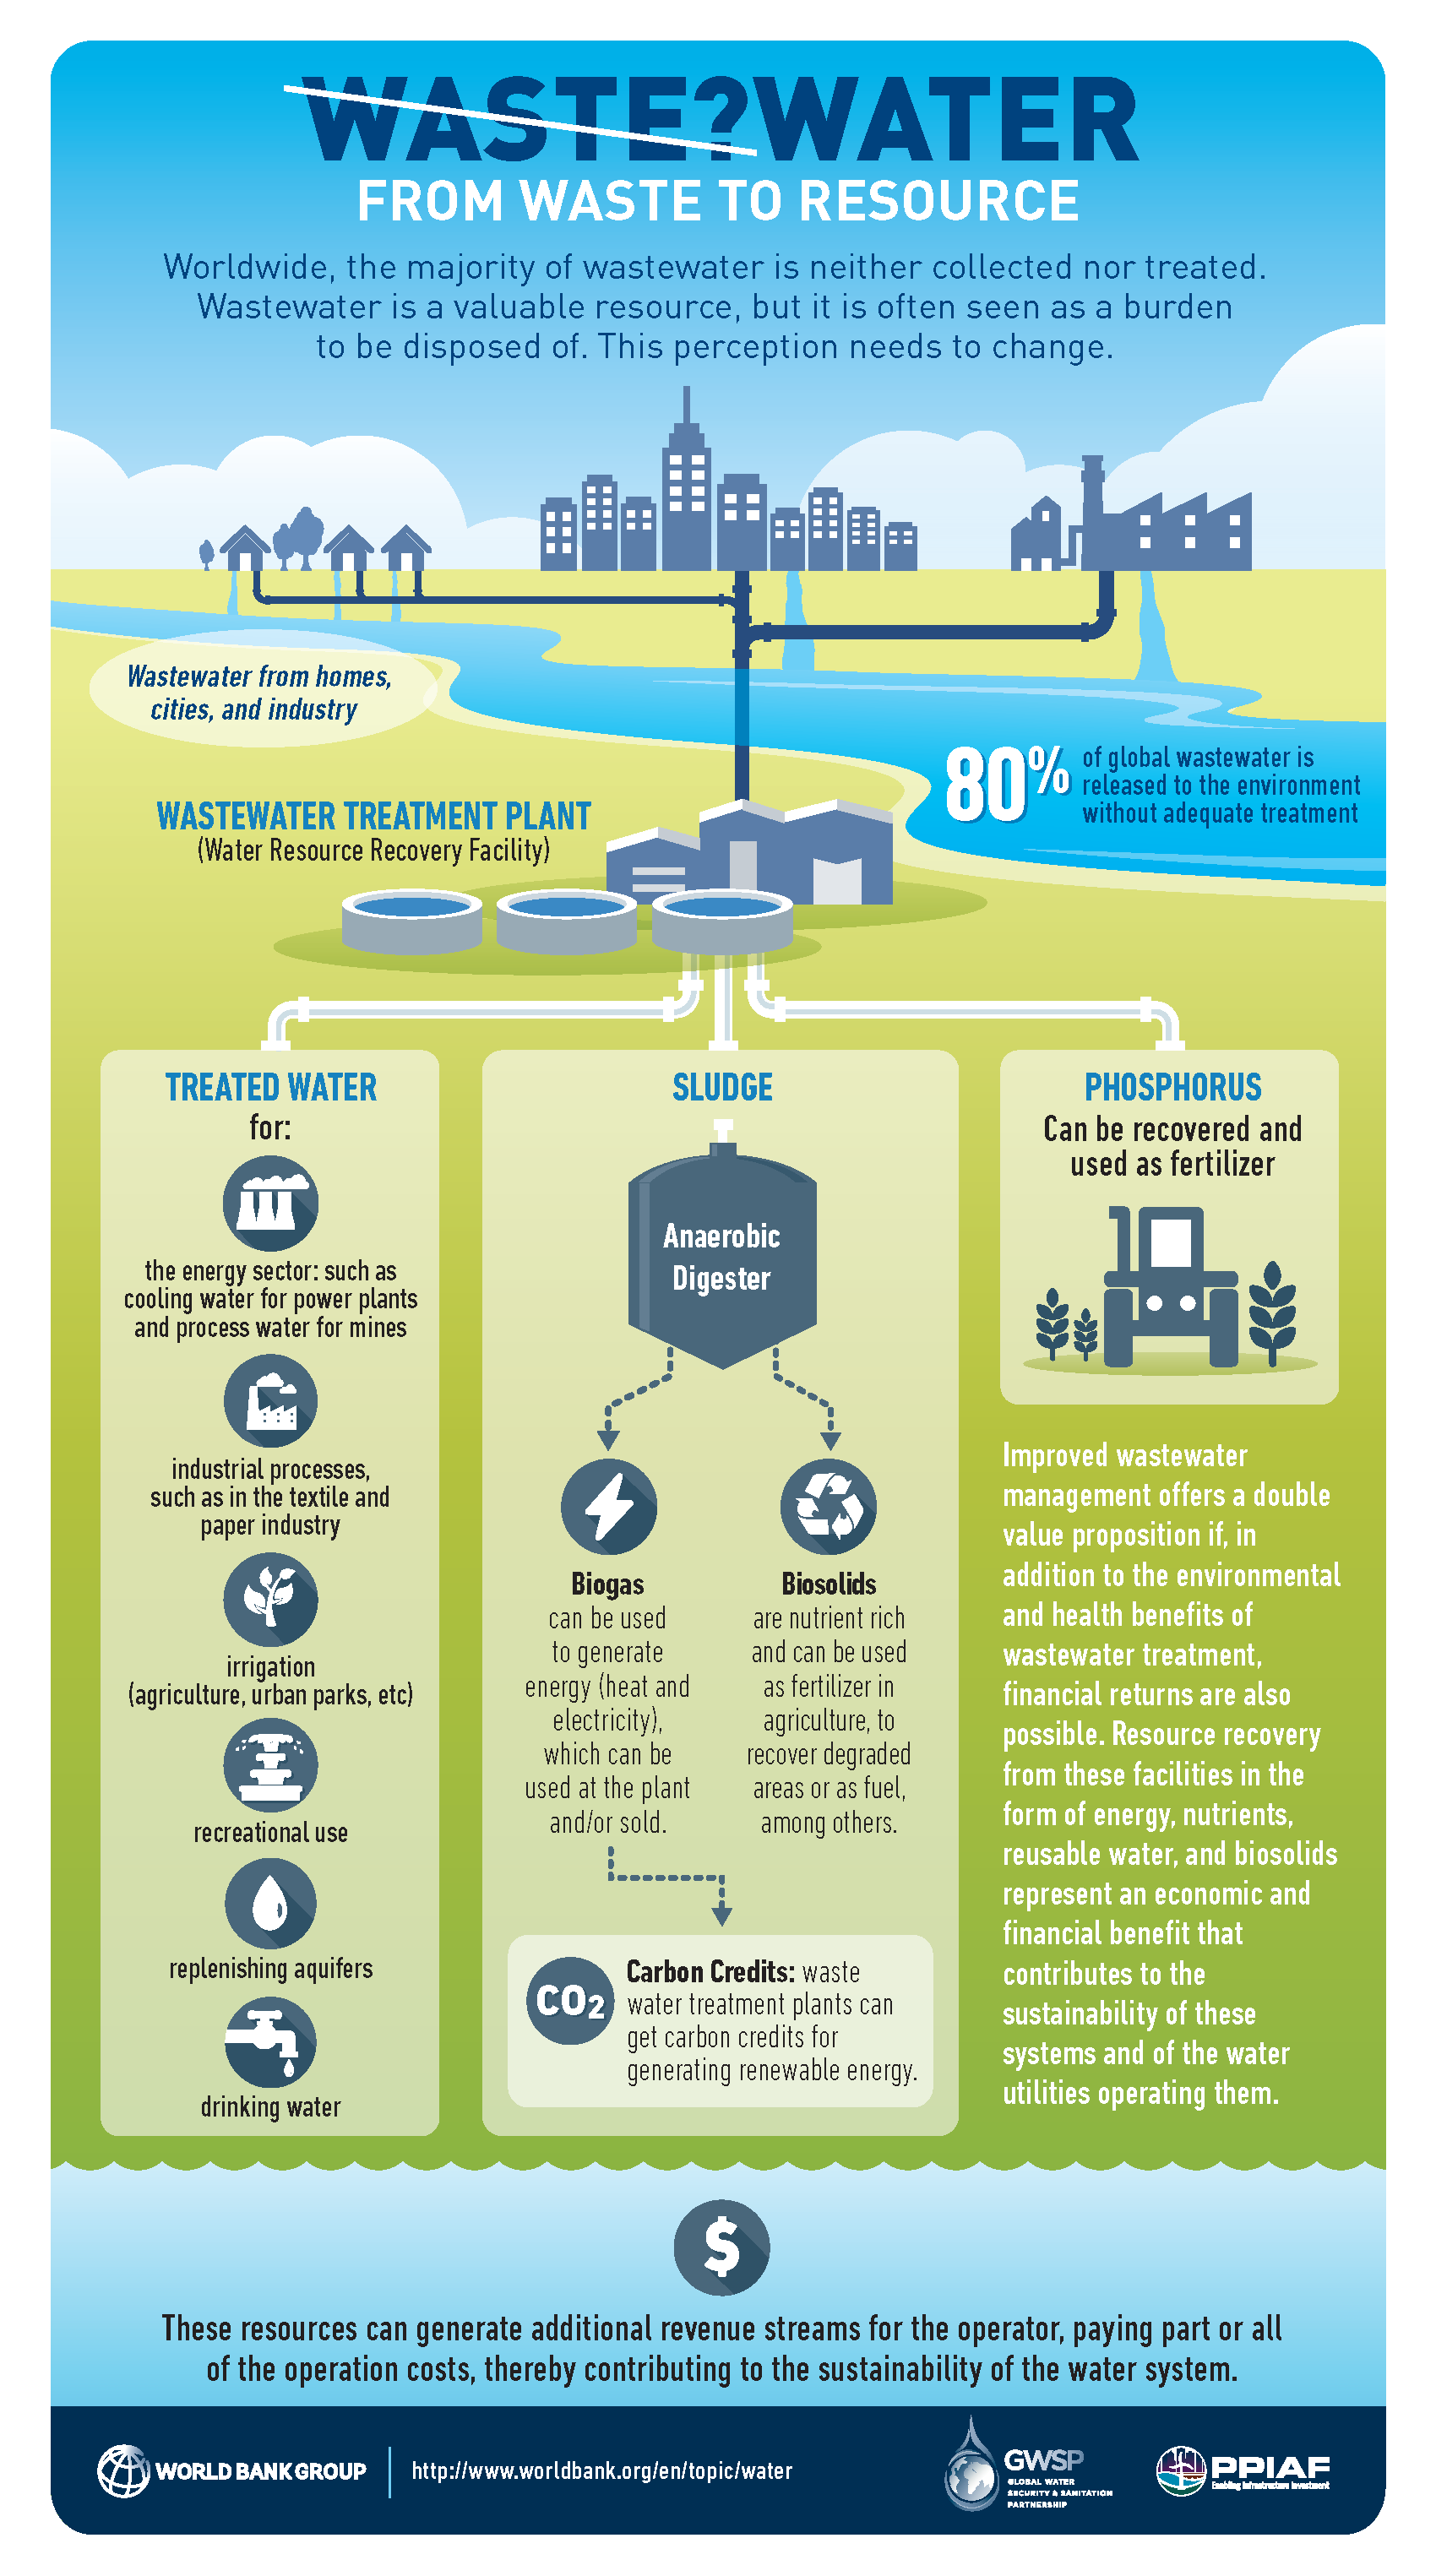
\includegraphics[scale=0.55]{WBWasteWaterResourceinfographic.png}\\
\emph{Source:  Waste to Resource - World Bank}\\
\end{center}









%\chapterimage{CareerChapterImage2.png}
\chapter{Wastewater Treatment - Careers}

\begin{itemize}
\item A career in wastewater treatment provides prospects of a stable and well paid employment with added perk of protecting the environment and the health of the community.
\item Wastewater treatment plants are facing challenges to fill the positions created by the retirement of the baby boomers.  It is estimated 30-50\% of the current employees will retire within the next 10 years.
\item There are a variety of career paths which require different skill sets and training. From high school graduates to PhDs.
\item Although actual renumeration and benefits depend on the size and location of the plant, in general wastewater jobs offer above average wages
\end{itemize}
\vspace{0.3cm}
\begin{tabular}{ |p{5cm}|p{5cm}|p{5cm}|  }
 \hline
 \multicolumn{3}{|c|}{Partial List of Wastewater Career Positions} \\
 \hline
 \hline
Plant Operators   & Collections Workers    &Electrical Maintenance Worker\\
Mechanical Mntnc. Worker   & Construction Inspectors   &Laboratory Technician\\
Environmental Specialists  & Civil Engineers & Mechanical Engineers\\
Electrical Engineers  & Office Assistants & Public Info. Specialists\\
Instrumentation Mntnc. Worker   & Finance and Accounting &Contracts Administrators\\
Warehouse Workers & Buyer & Health and Safety Specialist\\
Surveyors & CAD and Graphics Designers & Planners and Schedulers\\
 \hline
\end{tabular}\\



  
%% \section{Theorems}\index{Theorems}
%\part{Module 6}
%\chapterimage{Water1.png} % Chapter heading image

\chapter{Wastewater Math - Part II}
\chapterimage{MathCover.png} % Chapter heading image
\chapter{Wastewater Math}


% \begin{enumerate}
% \definecolor{shadecolor}{RGB}{200, 200, 240}
% \begin{snugshade*}
%\section{Units and Unit Conversion}\index{Units and Unit Conversion}
% 	\item \noindent\textsc{Units and Unit Conversion}
% \end{snugshade*}
\section{Unit Conversions}\index{Unit Conversions}
Common Units:\\

Length:  inches, ft, miles\\

Area:  ft$^2$, acres \\

Volume:  ft$^3$, gallons, acres-ft.\\

Density:  weight per volume, lbs/ft$^3$, lbs/gallon\\

Flow:  ft$^3$/min, MGD, acres-ft/day\\

		


Powers of Ten

\begin{center}
    
   
    \begin{tabular}{ | c | p{4cm} | c |p{8cm}|}
    \hline

%\hline
%\multicolumn{4}{|c|}{\textbf{ESSAYS}} \\
%\hline
%\thead{A Head} & \thead{A Second \\ Head} & \thead{A Third \\ Head} \\
%\hline%

$10^{12}$ & 1,000,000,000,000 & Tera & Like in tera byte drive - trillion\\
\hline 
$10^{9}$ & 1,000,000,000 & Giga & Like in giga byte data - billion\\
\hline
$10^{6}$ & 1,000,000 & Mega & Like in mega bytes or megawatts - million\\
\hline 
$10^{3}$ & 1,000 & Kilo & Like in kilogram \\
\hline 
$10^{0}$ & 1 &  & \\
\hline 
$10^{-3}$ & 0.001 & milli & Like in millimeter - thousandth of a meter\\
\hline 
$10^{-6}$ & 0.000001 & micro & Like in microgram - millionth of a gram \\
\hline 
$10^{-9}$ & 0.000000001 & nano & Like in nanometer - billionth of a meter\\
\hline 


    \end{tabular}
    
    \end{center}


For converting one measurement unit to another.

Step 1:  Make sure the original unit is for the same measurement as the conversion unit.  So if the original unit is for area, say ft$^2$ the conversion unit can be another area unit such as in$^2$ or acre but it cannot be gallons as gallon is a unit of volume.

Step 2: Write down the conversion formula as:

$Quantity \enspace in \enspace converted \enspace unit = Quantity \enspace (\cancel{Original \enspace Unit}) *   Conversion  \enspace Factor \enspace  \frac{Conversion \enspace unit}{\cancel{Original \enspace unit}}$


\section{Example Problems}
Problem 1\\
Convert 1000 $ft^3$ to cu. yards\\

$1000 \cancel{ft^3}*\frac{cu.yards}{27\cancel{ft^3}} = 37 cu.yards$

Problem 2\\
Convert 10 gallons/min to $ft^3$/hr\\

$\frac{10 \cancel{gallons}}{\cancel{min}}*  \frac{ft^3}{7.48 \cancel{gallons}}  * \frac{60 \cancel{min}}{hr}   = \frac{80.2ft^3}{hr}$


Problem 3\\
Convert 100,000 $ft^3$ to acre-ft.\\
$100,000 \cancel{ft^3} * \frac{acre-ft}{43,560 \cancel{ft^2-ft}} =  2.3 acre-ft$\\
\textbf{Note:} From the conversion table: acre = 43,560 $ft^2$\\
Thus, acre-ft  = 43,560 $ft^2$-ft\\

\section{Pounds Formula}\index{Pounds Formula}
%\section{Pounds Formula}\index{Pounds Formula}

% \begin{snugshade*}
% \item \noindent\textsc{Pounds Formula}
% \end{snugshade*}
Pounds formula is used for:
\begin{itemize}
\item Calculating the quantity in pounds of a particular wastewater constituent entering or leaving a wastewater treatment process
\item Calculating the pounds of chemicals to be added\\
\end{itemize}
So if the concentration of a particular constituent (in mg/liter) and the volume or flow of wastewater is given, one can calculate the amount of that constituent in pounds using the following – Pounds Formula:
$$lbs \enspace \textbf{or} \enspace \frac{lbs}{day}=concentration(\frac{mg}{l})*8.34*volume(MG) \enspace \textbf{or} \enspace flow(\frac{MG}{day}(MGD)$$

\begin{center}
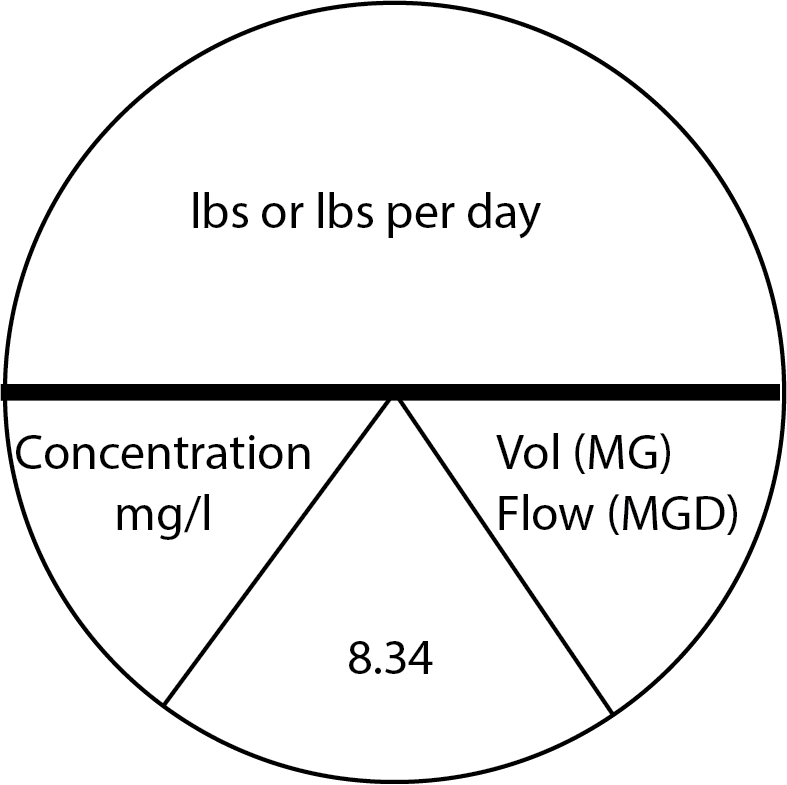
\includegraphics[scale=0.5]{PoundsFormula}
\end{center}

There are three variables – (lbs, concentration and volume) and one constant (8.34) in the pounds formula.  Knowing any of the two variables in the formula, one can calculate the third (unknown) variable by rearranging the equation.

\section{Concentration}\index{Concentration}

Concentration is typically expressed as mg/l which is the weight of the constituent (mg) in 1 l (liter) of solution (wastewater).  As 1 l of water weighs 1 million mg, a concentration of 1 mg/l implies 1 mg of constituent per 1 million mg of water or one part per million (ppm).   \textbf{Thus, mg/l and ppm are synonymous.}\\  
Sometimes the constituent concentration is expressed in terms of percentage.\\
\vspace{6pt}
For example:  sludge containing 5\% solids or a 12.5\% chlorine concentration solution.\\
\vspace{6pt}
As one liter of water weighs 1,000,000 mg, one percent of that weight is 10,000 mg.  So 1\% solids implies 10,000 mg of solids per liter or 10,000 mg/l or 10,000 ppm.\\
\vspace{6pt}
$1\% concentration = 10,000 \enspace ppm \enspace or \enspace\frac{mg}{l}$\\
$0.1\% concentration = 1,000 \enspace ppm \enspace or \enspace \frac{mg}{l}$\\
$0.01\% concentration = 100 \enspace ppm \enspace or \enspace \frac{mg}{l}$\\
$10\% concentration = 100,000 \enspace ppm \enspace or \enspace \frac{mg}{l}$\\
$5\% concentration = 50,000 \enspace ppm \enspace or \enspace \frac{mg}{l}$\\
$12.5\% concentration = 125,000 \enspace ppm \enspace or \enspace \frac{mg}{l}$

\subsection{Example Problems}
% \hl{Example Problems}\\

Problem 1\\Calculate the lbs/day of solids entering the plant given the influent flow is 5 MGD with an average solids concentration  of 250 mg/l.\\

Solution:\\

Applying lbs formula:\\
$\dfrac{lbs}{day}=5 MGD *250\dfrac{mg}{l}*8.34 = \boxed{10,425\dfrac{lbs}{day}}$
\\
Problem 2\\Calculate the lbs of solids in the primary sludge if the sludge flow is 7500 gallons and the solids concentration is 4.5\%.\\
Solution\\
Applying lbs formula:\\
$lbs \enspace solids = \dfrac{7500}{1,000,000}MG * 4.5*10,000 *8.34 = \boxed{2,815 \enspace lbs \enspace solids}$\\
\textbf{Note:}\\  
1) 7500 gallons was converted to MG by dividing by 1,000,000\\
$7500 \enspace gallons * \dfrac{1 MG}{1,000,000 \enspace gallon}$\\
2) 4.5\% was converted to mg/l by multiplying by 10,000 as 1\%=10,000mg/l

\newpage
\section{Area \& Volume}\index{Area \& Volume}
% \section{Area \& Volume}\index{Area \& Volume}

% \begin{snugshade*}
% 	\item \noindent\textsc{Area \& Volume}
% \end{snugshade*}

\begin{center}
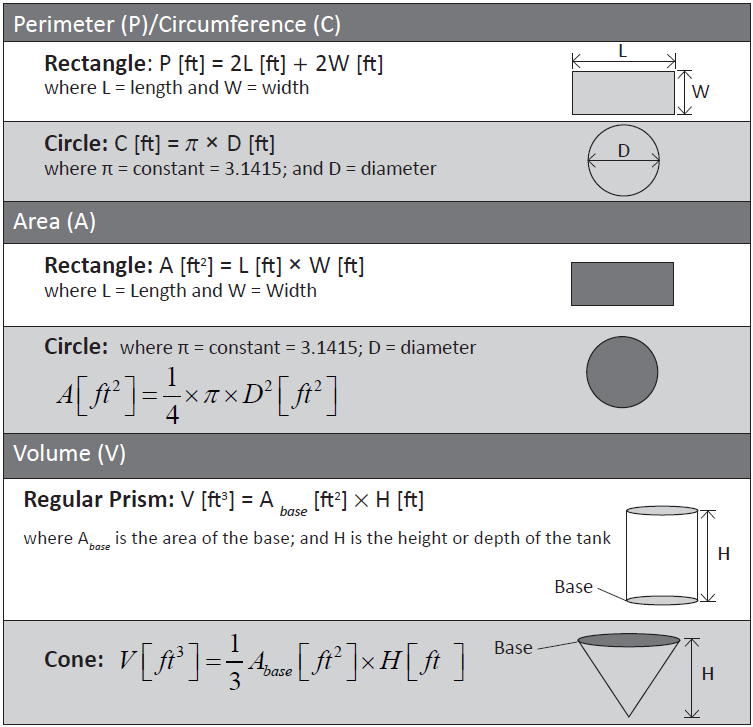
\includegraphics[scale=0.5]{Area&VolumeFormula}
\end{center}
\subsection{Example Problems}
% \hl{Example Problems}\\
\begin{enumerate}

\item The floor of a rectangular building is 20 feet long by 12 feet wide and the inside walls are 10 feet high. Find the total surface area of the inside walls of this building\\
Solution:\\
% \begin{center}
\begin{tikzpicture}
	%%% Edit the following coordinate to change the shape of your
	%%% cuboid
      
	%% Vanishing points for perspective handling
	\coordinate (P1) at (-7cm,1.5cm); % left vanishing point (To pick)
	\coordinate (P2) at (8cm,1.5cm); % right vanishing point (To pick)

	%% (A1) and (A2) defines the 2 central points of the cuboid
	\coordinate (A1) at (0em,0cm); % central top point (To pick)
	\coordinate (A2) at (0em,-2cm); % central bottom point (To pick)

	%% (A3) to (A8) are computed given a unique parameter (or 2) .8
	% You can vary .8 from 0 to 1 to change perspective on left side
	\coordinate (A3) at ($(P1)!.8!(A2)$); % To pick for perspective 
	\coordinate (A4) at ($(P1)!.8!(A1)$);

	% You can vary .8 from 0 to 1 to change perspective on right side
	\coordinate (A7) at ($(P2)!.7!(A2)$);
	\coordinate (A8) at ($(P2)!.7!(A1)$);

	%% Automatically compute the last 2 points with intersections
	\coordinate (A5) at
	  (intersection cs: first line={(A8) -- (P1)},
			    second line={(A4) -- (P2)});
	\coordinate (A6) at
	  (intersection cs: first line={(A7) -- (P1)}, 
			    second line={(A3) -- (P2)});

	%%% Depending of what you want to display, you can comment/edit
	%%% the following lines

	%% Possibly draw back faces

	\fill[gray!40] (A2) -- (A3) -- (A6) -- (A7) -- cycle; % face 6
	\node at (barycentric cs:A2=1,A3=1,A6=1,A7=1) {\tiny Floor=W*L};
	
	\fill[gray!50] (A3) -- (A4) -- (A5) -- (A6) -- cycle; % face 3
	\node at (barycentric cs:A3=1,A4=1,A5=1,A6=1) {\tiny Wall - W*H};
	
	\fill[gray!10, opacity=0.2] (A5) -- (A6) -- (A7) -- (A8) -- cycle; % face 4
	\node at (barycentric cs:A5=1,A6=1,A7=1,A8=1) {\tiny Wall - L*H};
	
	\fill[gray!10,opacity=0.5] (A1) -- (A2) -- (A3) -- (A4) -- cycle; % f2
	\node at (barycentric cs:A1=1,A2=1,A3=1,A4=1) {\tiny Wall - L*H};
	
	\fill[gray!40,opacity=0.2] (A1) -- (A4) -- (A5) -- (A8) -- cycle; % f5
	\node at (barycentric cs:A1=1,A4=1,A5=1,A8=1) {\tiny Ceiling=W*L};	
	
	\draw[thick,dashed] (A5) -- (A6);
	\draw[thick,dashed] (A3) -- (A6);
	\draw[thick,dashed] (A7) -- (A6);

	%% Possibly draw front faces

	%\fill[orange] (A1) -- (A8) -- (A7) -- (A2) -- cycle; % face 1
	\node at (barycentric cs:A1=1,A8=1,A7=1,A2=1) {\tiny Wall - W*H};
	


	%% Possibly draw front lines
	\draw[thick] (A1) -- (A2);

	\draw[<->] (-1.8,0.38) -- (-1.8,-1.3)node [midway, above=-1.8mm] {\hspace{-1.3cm}\tiny Height=10'};
	\draw[<->] (-1.6,-1.4) -- (-.3,-2.1)node [midway, above=-2.6mm] {\hspace{-1.3cm}\tiny Length=20'};
	\draw[<->] (2.6,-1.13) -- (0.2,-2.2)node [midway, below=.6mm] {\hspace{1.2cm}\tiny Width=12'};
	\draw[thick] (A3) -- (A4);
	\draw[thick] (A7) -- (A8);
	\draw[thick] (A1) -- (A4);
	\draw[thick] (A1) -- (A8);
	\draw[thick] (A2) -- (A3);
	\draw[thick] (A2) -- (A7);
	\draw[thick] (A4) -- (A5);
	\draw[thick] (A8) -- (A5);
	
	% Possibly draw points
	% (it can help you understand the cuboid structure)
%	\foreach \i in {1,2,...,8}
%	{
%	  \draw[fill=black] (A\i) circle (0.15em)
%	    node[above right] {\tiny \i};
%	}
	% \draw[fill=black] (P1) circle (0.1em) node[below] {\tiny p1};
	% \draw[fill=black] (P2) circle (0.1em) node[below] {\tiny p2};
\end{tikzpicture}\\
% \end{center}
2 Walls W*H + 2 Walls L*H= $2*12*10ft^2 + 2*20*10ft^2$\\
$=240+400=\boxed{640ft^2}$

2 Walls W*H + 2 Walls L*H + Floor + Ceiling= $2*12*10ft^2 + 2*20*10ft^2 + 2*12*20ft^2$\\
$=240+400+480=\boxed{1,120ft^2}$

\item How many gallons of paint will be required to paint the inside walls of a 40 ft long x 65 ft wide x 20 ft high tank if the paint coverage is 150 sq. ft per gallon.  Note:  We are painting walls only.  Disregard the floor and roof areas.
Solution:\\
\vspace{0.3cm}
% \begin{center}
\begin{tikzpicture}
	%%% Edit the following coordinate to change the shape of your
	%%% cuboid
      
	%% Vanishing points for perspective handling
	\coordinate (P1) at (-7cm,1.5cm); % left vanishing point (To pick)
	\coordinate (P2) at (8cm,1.5cm); % right vanishing point (To pick)

	%% (A1) and (A2) defines the 2 central points of the cuboid
	\coordinate (A1) at (0em,0cm); % central top point (To pick)
	\coordinate (A2) at (0em,-2cm); % central bottom point (To pick)

	%% (A3) to (A8) are computed given a unique parameter (or 2) .8
	% You can vary .8 from 0 to 1 to change perspective on left side
	\coordinate (A3) at ($(P1)!.8!(A2)$); % To pick for perspective 
	\coordinate (A4) at ($(P1)!.8!(A1)$);

	% You can vary .8 from 0 to 1 to change perspective on right side
	\coordinate (A7) at ($(P2)!.7!(A2)$);
	\coordinate (A8) at ($(P2)!.7!(A1)$);

	%% Automatically compute the last 2 points with intersections
	\coordinate (A5) at
	  (intersection cs: first line={(A8) -- (P1)},
			    second line={(A4) -- (P2)});
	\coordinate (A6) at
	  (intersection cs: first line={(A7) -- (P1)}, 
			    second line={(A3) -- (P2)});

	%%% Depending of what you want to display, you can comment/edit
	%%% the following lines

	%% Possibly draw back faces

	\fill[gray!40] (A2) -- (A3) -- (A6) -- (A7) -- cycle; % face 6
	\node at (barycentric cs:A2=1,A3=1,A6=1,A7=1) {};
	
	\fill[gray!50] (A3) -- (A4) -- (A5) -- (A6) -- cycle; % face 3
	\node at (barycentric cs:A3=1,A4=1,A5=1,A6=1) {\tiny Wall - W*H};
	
	\fill[gray!10, opacity=0.2] (A5) -- (A6) -- (A7) -- (A8) -- cycle; % face 4
	\node at (barycentric cs:A5=1,A6=1,A7=1,A8=1) {\tiny Wall - L*H};
	
	\fill[gray!10,opacity=0.5] (A1) -- (A2) -- (A3) -- (A4) -- cycle; % f2
	\node at (barycentric cs:A1=1,A2=1,A3=1,A4=1) {\tiny Wall - L*H};
	
	\fill[gray!40,opacity=0.2] (A1) -- (A4) -- (A5) -- (A8) -- cycle; % f5
	\node at (barycentric cs:A1=1,A4=1,A5=1,A8=1) {};	
	
	\draw[thick,dashed] (A5) -- (A6);
	\draw[thick,dashed] (A3) -- (A6);
	\draw[thick,dashed] (A7) -- (A6);

	%% Possibly draw front faces

	%\fill[orange] (A1) -- (A8) -- (A7) -- (A2) -- cycle; % face 1
	\node at (barycentric cs:A1=1,A8=1,A7=1,A2=1) {\tiny Wall - W*H};
	


	%% Possibly draw front lines
	\draw[thick] (A1) -- (A2);

	\draw[<->] (-1.8,0.38) -- (-1.8,-1.3)node [midway, above=-1.8mm] {\hspace{-1.3cm}\tiny Height=20'};
	\draw[<->] (-1.6,-1.4) -- (-.3,-2.1)node [midway, above=-2.6mm] {\hspace{-1.3cm}\tiny Length=45'};
	\draw[<->] (2.6,-1.13) -- (0.2,-2.2)node [midway, below=.6mm] {\hspace{1.2cm}\tiny Width=65'};
	\draw[thick] (A3) -- (A4);
	\draw[thick] (A7) -- (A8);
	\draw[thick] (A1) -- (A4);
	\draw[thick] (A1) -- (A8);
	\draw[thick] (A2) -- (A3);
	\draw[thick] (A2) -- (A7);
	\draw[thick] (A4) -- (A5);
	\draw[thick] (A8) -- (A5);
	
	% Possibly draw points
	% (it can help you understand the cuboid structure)
%	\foreach \i in {1,2,...,8}
%	{
%	  \draw[fill=black] (A\i) circle (0.15em)
%	    node[above right] {\tiny \i};
%	}
	% \draw[fill=black] (P1) circle (0.1em) node[below] {\tiny p1};
	% \draw[fill=black] (P2) circle (0.1em) node[below] {\tiny p2};
\end{tikzpicture}\\
% \end{center}
\vspace{0.3cm}
2 Walls W*H + 2 Walls L*H = $2*65*20ft^2 + 2*40*20ft^2= 2,600+1,600=4,200ft^2$\\
$\implies @150\dfrac{ft^2}{gal} \enspace paint \enspace coverage \enspace \rightarrow \enspace \dfrac{4,200\cancel{ft^2}}{150\dfrac{\cancel{ft^2}}{gal}}=\boxed{28 \enspace gallons}$
\vspace{0.3cm}
\item What is the circumference of a 100 ft diameter circular clarifier?\\
\vspace{0.3cm}
Solution:\\
\vspace{0.3cm}
$Circumference=\pi*D=3.14*100ft=\boxed{314ft}$
\vspace{0.3cm}
\item If the surface area of a clarifier is 5,025$ft^2$, what is its diameter?\\
\vspace{0.3cm}
Solution:\\
\vspace{0.3cm}
$Surface \enspace area=\dfrac{\pi}{4}*D^2 \enspace \implies 5025(ft^2)=0.785*D^2 (ft^2)$\\
$\implies D^2=\dfrac{5025}{0.785} \implies D=\sqrt{6401.3}=\boxed{80ft}$
\vspace{0.3cm}

\item How many gallons of wastewater would 600 feet of 6-inch diameter pipe hold, approximately?\\
\vspace{0.3cm}
Solution:\\

\vspace{0.3cm}
% \begin{center}
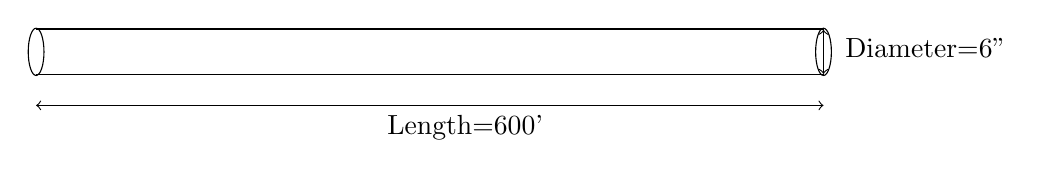
\begin{tikzpicture}
\draw (0,0) ellipse (0.1cm and 0.3cm);
\draw (10,0) ellipse (0.1cm and 0.3cm);
\draw [-] (0,-0.29) -- (10,-0.29);
\draw [-] (0,0.29) -- (10,0.29);
\draw [<->] (10,-0.28) -- (10,0.28) node [midway, below=-3mm] {\hspace{2.6cm}Diameter=6"};
\draw [<->] (0,-.68) -- (10,-.68)node [midway, below] {\hspace{0.9cm}Length=600'};
\end{tikzpicture}
% \end{center}
\vspace{0.3cm}
$Volume=\dfrac{\pi}{4}D^2*L=0.785*\Big(\dfrac{6}{12}\Big)^2*600\cancel{ft^3}*7.48\dfrac{gallons}{\cancel{ft^3}}=\boxed{881 \enspace gallons}$
\newpage
\item A 110 ft diameter digester with a 12 ft deep cone is operated at a side water depth of 20 ft.  Caluclate the volume of sludge in the digester in $ft^3$ and gallons.\\
\vspace{0.3cm}
Solution:\\
\vspace{0.3cm}
% \begin{center}
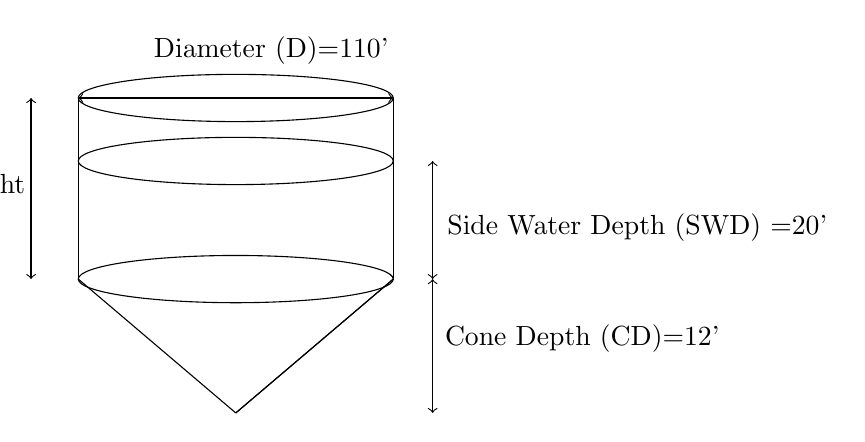
\begin{tikzpicture}
\draw (0,0) ellipse (2cm and 0.3cm);
\draw (0,-2.3) ellipse (2cm and 0.3cm);
\draw (0,-.8) ellipse (2cm and 0.3cm);
\draw [-] (2,-2.3) -- (2,0);
\draw [<->] (-2,0) -- (2,0) node [midway, below=-0.9cm] {\hspace{0.9cm}Diameter (D)=110'}; 
\draw [<->] (-2.6,-2.3) -- (-2.6,0) node [midway, below=-.3cm] {\hspace{-2.6cm}Cylinder Height};
\draw [<->] (2.5,-2.3) -- (2.5,-0.8) node [midway, below=-0.2cm] {\hspace{5.2cm}Side Water Depth (SWD) =20'};
\draw [-] (0,-4) -- (2,-2.3);
\draw [-] (0,-4) -- (-2,-2.3);
\draw [-] (0,-4) -- (2,-2.3);
\draw [-] (-2,0) -- (-2,-2.3);
\draw [<->] (2.5,-2.3) -- (2.5,-4)node [midway, below=-0.4cm] {\hspace{3.8cm}Cone Depth (CD)=12'};
\end{tikzpicture}\\
% \end{center}
$Digester \enspace volume=Volume_{cylinder}+Volume_{cone}$\\
$\implies Digester \enspace volume=\dfrac{\pi}{4}D^2*SWD+\dfrac{1}{3}*\Bigg(\dfrac{\pi}{4}*D^2*CD\Bigg)$\\
\vspace{0.3cm}
$=0.785*110^2*20+1.05*110^2*12=\boxed{227,988ft^3}$\\
\vspace{0.3cm}
$227,988\cancel{ft^3}*7.48\dfrac{gallons}{\cancel{ft^3}}=\boxed{1,705,352 \enspace gallons}$
\end{enumerate}

\section{Process Removal Efficiency}\index{Process Removal Efficiency}

% \section{Process Removal Efficiency}\index{Process Removal Efficiency}
% \begin{snugshade*}
% 	\item \noindent\textsc{Process Removal Efficiency}
% \end{snugshade*}
\begin{itemize}
\item Process removal rate or removal efficiency is the percentage of the inlet concentration removed.  
\item It is used for quantifying the pollutant removal during wastewater treatment and is established based upon the amount of a particular wastewater constituent entering and leaving a treatment process.

\item $Process \enspace Removal \enspace Rate \enspace (\%) = \dfrac{Pollutant \enspace  In-Pollutant\enspace  Out}{Pollutant \enspace In}*100$\\

\item If 10 units of a pollutant are entering a process and 8 units of pollutant are leaving (process removes 2 units), then the process removal rate for that pollutant is (10-8)/10*100=20\%.  In this example the process is 20\% efficient in removing that particular pollutant.

\item The amount of pollutant can be measured in terms of concentration (mg/l) or in terms of mass loading (lbs).  The pounds formula is used for calculating the mass loadings.  
\end{itemize}
The above example is for calculating the removal efficiency using the inlet and outlet concentrations or mass loading.\\
The methods below can be used for calculating either the inlet or outlet pollutant concentrations, if the removal efficiency and the corresponding inlet or outlet concentrations are given. 


\hl{Case 1:  Calculating outlet conc. (X) given the inlet conc. and removal efficiency (RE\%):}

\tikzstyle{block} = [rectangle, draw, fill=red!40, 
    text width=6em, text centered, rounded corners, minimum height=3em]
\tikzstyle{arrow} = [draw, -latex']
\begin{figure}[!h]
\centering
\begin{tikzpicture}[node distance =1.5cm, auto]
    \draw ++(0,0) node [block] (Process) {Process};
   \node[node distance=1.9in] (dummy_in) [left of=Process] {In};
   \node[node distance=1.9in] (dummy_out) [right of=Process] {Out};
	\node (Removal) [below of=Process, yshift=-0in] {${Removal \enspace Efficiency=RE\% \enspace (Given)}$};
    \path [arrow] (dummy_in)-- (Process)  node [above] {\hspace{-5.8cm}$A \enspace mg/l \enspace (Given) $} node [below] {\hspace{-5.8cm}$100 \enspace mg/l$};
    \path [arrow] (Process) -- (dummy_out)  node [above] {\hspace{-4cm}$X \enspace mg/l \enspace (Unknown)$} node [below] {\hspace{-3.9cm}($100-RE\%)\enspace mg/l$};
   \draw[arrow] (Process) -- (Removal);
\end{tikzpicture}
\end{figure}
Using the fact that if the inlet concentration was 100 mg/l, the outlet concentration would be 100 minus the removal efficiency.\\
Setup the equation as:  $\dfrac{Out}{In}: \enspace \dfrac{X \enspace mg/l}{A \enspace mg/l}=\dfrac{100-RE\%}{100}$\\
Calculate X using cross multiplication - if $\dfrac{A}{B}=\dfrac{C}{D} \implies A=B*\dfrac{C}{D}$:\\
$X \enspace mg/l=A \enspace mg/l*\dfrac{100-RE\%}{100}$\\


\hl{Case 2:  Calculating inlet conc. (X) given the outlet conc. and removal efficiency (RE\%):}

\begin{figure}[!h]
\centering
\begin{tikzpicture}[node distance =1.5cm, auto]
    \draw ++(0,0) node [block] (Process) {Process};
   \node[node distance=1.9in] (dummy_in) [left of=Process] {In};
   \node[node distance=1.9in] (dummy_out) [right of=Process] {Out};
	\node (Removal) [below of=Process, yshift=-0in] {$Removal \enspace Efficiency=RE\% \enspace (Given)$};
    \path [arrow] (dummy_in)-- (Process)  node [above] {\hspace{-5.8cm}$X \enspace mg/l \enspace (Unknown)$} node [below] {\hspace{-5.8cm}$100 \enspace mg/l$};
    \path [arrow] (Process) -- (dummy_out)  node [above] {\hspace{-4cm}$A \enspace mg/l \enspace (Given)$} node [below] {\hspace{-3.9cm}($100-RE\%)\enspace mg/l$};
   \draw[arrow] (Process) -- (Removal);
\end{tikzpicture}
\end{figure}
Using the fact that if the inlet concentration was 100 mg/l, the outlet concentration would be 100 minus the removal efficiency.\\
Setup the equation as:  $\dfrac{In}{Out}: \enspace \dfrac{X \enspace mg/l}{A \enspace mg/l}=\dfrac{100}{100-RE\%}$\\
\vspace{0.3cm}
Calculate X using cross multiplication - if $\dfrac{A}{B}=\dfrac{C}{D} \implies A=B*\dfrac{C}{D}$:\\
$X \enspace mg/l=A \enspace mg/l*\dfrac{100}{100-RE\%}$\\

\vspace{0.4cm}
\subsection{Example Problems}
% \hl{Example Problems:}\\

\begin{enumerate}

\item What is the \% removal efficiency if the influent concentration is 10 mg/L and the effluent concentration is 2.5 mg/L?\\
$Removal \enspace Rate (\%) = \dfrac{In-Out}{In}*100 \implies \dfrac{10-2.5}{10}*100=\boxed{75\%}$



\item Calculate the outlet concentration if the inlet concentration is 80 mg/l and the process removal efficiency is 60\%\\
Solution:\\

\tikzstyle{block} = [rectangle, draw, fill=red!40, 
    text width=6em, text centered, rounded corners, minimum height=3em]
\tikzstyle{arrow} = [draw, -latex']
\begin{figure}[!h]
\centering
\begin{tikzpicture}[node distance =1.5cm, auto]
    \draw ++(0,0) node [block] (Process) {Process};
   \node[node distance=1.5in] (dummy_in) [left of=Process] {In};
   \node[node distance=1.5in] (dummy_out) [right of=Process] {Out};
	\node (Removal) [below of=Process, yshift=-0in] {$Removal \enspace Efficiency=60\%$};
    \path [arrow] (dummy_in)-- (Process)  node [above] {\hspace{-4.39cm}$80mg/l$} node [below] {\hspace{-4.39cm}$100mg/l$};
    \path [arrow] (Process) -- (dummy_out)  node [above] {\hspace{-3.cm}$Xmg/l$} node [below] {\hspace{-3cm}40mg/l};
   \draw[arrow] (Process) -- (Removal);
\end{tikzpicture}
%\caption[MFCC]{Diagrama en bloques del cálculo de las MFCC para un frame.}
%\label{MFCC}
\end{figure}

$\dfrac{Out}{In} \enspace:\enspace\dfrac{Actual \enspace Outlet (X)}{80}=\dfrac{100-60}{100}$\\
$\implies \dfrac{Actual \enspace Outlet (X)}{80} =0.4$\\
$\implies Actual \enspace  Outlet (X) = 0.4 * 80 = \boxed{32 mg/l}$\\


\item Calculate the inlet concentration if the outlet concentration is 80 mg/l and the process removal efficiency is 60\%\\

\tikzstyle{block} = [rectangle, draw, fill=red!40, 
    text width=6em, text centered, rounded corners, minimum height=3em]
\tikzstyle{arrow} = [draw, -latex']
\begin{figure}[!h]
\centering
\begin{tikzpicture}[node distance =1.5cm, auto]
    \draw ++(0,0) node [block] (Process) {Process};
   \node[node distance=1.5in] (dummy_in) [left of=Process] {In};
   \node[node distance=1.5in] (dummy_out) [right of=Process] {Out};
	\node (Removal) [below of=Process, yshift=-0in] {$Removal \enspace Efficiency=60\%$};
    \path [arrow] (dummy_in)-- (Process)  node [above] {\hspace{-4.39cm}$Xmg/l$} node [below] {\hspace{-4.39cm}$100mg/l$};
    \path [arrow] (Process) -- (dummy_out)  node [above] {\hspace{-3.cm}80mg/l} node [below] {\hspace{-3cm}40mg/l};
   \draw[arrow] (Process) -- (Removal);
\end{tikzpicture}
\end{figure}

$\dfrac{In}{Out} \enspace : \enspace \dfrac{Actual \enspace inlet \enspace  (X)}{80}=\dfrac{100}{100-60}\implies \dfrac{Actual \enspace inlet \enspace  (X)}{80}=2.5$\\    
Rearranging the equation:   $Actual \enspace inlet (X)=2.5*80 = \boxed{200 mg/l}$\\

\item If a plant removes 35\% of the influent BOD in the primary treatment and 85\% of the remaining BOD in the secondary system, what is the BOD of the raw wastewater if the BOD of the final effluent is 20mg/l\\
Solution:\\

\begin{figure}[!h]
\centering
\begin{tikzpicture}[node distance =1.5cm, auto]
    \draw ++(0,0) node [block] (Primary) {Primary};
    
   \node[node distance=1.9in] (dummy_in) [left of=Primary] {Influent BOD};
   \node[node distance=1.9in] (dummy_out) [right of=Primary] {Primary BOD Out};
	\node (Removal) [below of=Primary, yshift=-0in] {$Removal \enspace Efficiency=35\% $};
    \path [arrow] (dummy_in)-- (Primary)  node [above] {\hspace{-4.8cm}$X \enspace mg/l \enspace$} node [below] {};
    \path [arrow] (Primary) -- (dummy_out)  node [above] {\hspace{-4.9cm}$0.65X \enspace mg/l$} node [below] {};
   \draw[arrow] (Process) -- (Removal);
\end{tikzpicture}
\end{figure}


\begin{figure}[!h]
\centering
\begin{tikzpicture}[node distance =1.5cm, auto]
    \draw ++(0,0) node [block] (Secondary) {Secondary};
    
   \node[node distance=1.9in] (dummy_in) [left of=Secondary] {Primary BOD Out};
   \node[node distance=1.9in] (dummy_out) [right of=Secondary] {Secondary BOD Out};
	\node (Removal) [below of=Secondary, yshift=-0in] {$Removal \enspace Efficiency=85\% $};
    \path [arrow] (dummy_in)-- (Secondary)  node [above] {\hspace{-4.8cm}$0.65X \enspace mg/l \enspace$} node [below] {\hspace{-5cm}$100 \enspace mg/l$};
    \path [arrow] (Secondary) -- (dummy_out)  node [above] {\hspace{-4.9cm}$20 \enspace mg/l$} node [below] {\hspace{-4.9cm}$15 \enspace mg/l$};
   \draw[arrow] (Process) -- (Removal);
\end{tikzpicture}
\end{figure}
\vspace{0.3cm}
For the Secondary process:\\
$\dfrac{In}{Out}: \enspace \dfrac{0.65X}{20}=\dfrac{100}{15} \implies X \enspace mg/l=\dfrac{100*20}{15*0.65}=\boxed{205 \enspace mg/l}$\\

\vspace{0.3cm}
Alternate Solution \#1

$\xrightarrow[
				\text{X}\dfrac{mg}{l}
			]
			{
			\text{Influent BOD}
			}
 \boxed{Primary}
 \xrightarrow[
 				\text{X-0.35X=X*(1-0.35)=0.65X}\dfrac{mg}{l}
 			]
 			{
 			\text{Primary Effluent BOD}
 			}
 \boxed{Secondary}
 \xrightarrow[
				\text{0.65X-0.5525X=(0.65-0.5525)X=0.0975X }
			 ]
			{
			\text{Secondary Effluent BOD}
			}
$\\
\hspace{2.8cm}$\downarrow$ {\tiny(0.35X)BOD Removed}\hspace{3.2cm}$\downarrow$ {\tiny(0.65*0.85)X = 0.5525X BOD Removed}\\
$\implies 0.0975X=20 \implies X=\dfrac{20}{0.0975}=\boxed{205\dfrac{mg}{l}}$\\

\vspace{0.3cm}

Alternate Solution \#2:\\
$\xrightarrow[\text{X}\dfrac{mg}{l}]{\text{Influent BOD}}\boxed{Primary}\xrightarrow[\text{0.65X}]{\text{Primary Effluent BOD}}\boxed{Secondary}\xrightarrow[\text{(0.65*0.15)X}]{\text{Secondary Effluent BOD}}$\\
\hspace{2.8cm}$\downarrow$ {\tiny(0.35X)BOD Removed}\hspace{2.2cm}$\downarrow$ {\tiny(0.65X*0.85)BOD Removed}\\

Primary Effluent BOD = Influent BOD * (1-Primary BOD Removal), and\\
Secondary Effluent BOD=[Primary Effluent BOD]*(1-Secondary BOD Removal)\\
Secondary Eff. BOD=[Influent BOD * (1-Primary BOD Removal)]*(1-Secondary BOD Removal)\\

Therefore, 20 = [X*(1-0.35)] * (1-0.85)= X*0.65*0.15\\
$\implies 20 \enspace \dfrac{mg}{l}= 0.0975X \implies X=\dfrac{20}{0.0975}=\boxed{205 \enspace \dfrac{mg}{l}}$

\end{enumerate}
\section{Pumping}\index{Pumping}
% \section{Pumping}\index{Pumping}
% \pagebreak
% \begin{snugshade*}
% 	\item \noindent\textsc{Pumping}
% \end{snugshade*}
For Grades I \& II, pumping rate problems include the following:
% \begin{enumerate}
% \definecolor{shadecolor}{RGB}{225, 235, 235}
% \begin{snugshade*}
% \item \noindent\textsc{Calculating volume pumped in a given time interval given the pump flow rate\\}
% \end{snugshade*}
\subsection{Calculating volume pumped given the pump flow rate}\index{Calculating volume pumped given the pump flow rate}

\textbf{Method:\\}
\hspace{1cm}Step 1. Multiply the pump flow rate by the time interval\\
\textbf{Make sure:}
\begin{itemize}
\item The time units - in the given time interval and in the pump flow rate match
\end{itemize}
\subsection{Calculating time to pump a certain volume}\index{Calculating time to pump a certain volume}
% \begin{snugshade*}
% \item \noindent\textsc{Calculating time to pump a certain volume given the pump flow rate\\}
% \end{snugshade*}
\textbf{Method:}
\hspace{1cm}Step 1. Calculate the total volume pumped\\
\hspace{1cm}Step 2.	Divide the total volume by the pump flow rate\\
\textbf{Make sure:}
\begin{itemize}
\item The volume units - in the volume that needs to be pumped and in the pump flow rate match
\item The time unit in the pump flow rate needs to be converted to the time unit that you need the answer in
\end{itemize}
% \end{enumerate}

\section{Example Problems}
% \hl{Example Problems:}\\

\begin{enumerate}

\item A sludge pump is set to pump 5 minutes each hour. It pumps at the rate of 35 gpm. How many gallons of sludge are pumped each day?\\
Solution:\\
$\dfrac{35 \enspace gal \enspace sludge}{\cancel{min}}*\dfrac{5 \enspace \cancel{min}}{\cancel{hr}} *\dfrac{24 \enspace \cancel{hr}}{day}=\boxed{\dfrac{4,200 \enspace gallons}{day}}$\\
\vspace{0.5cm}

\item A sludge pump operates 5 minutes each 15 minute interval.  If the pump capacity is 60 gpm, how many gallons of sludge are pumped daily?

$\dfrac{60 \enspace gal \enspace sludge}{\xcancel{min}}*\dfrac{5 \enspace \xcancel{min}}{15 \enspace \cancel{min}}*1440\dfrac{\cancel{min}}{day}=\boxed{\dfrac {28,800 \enspace gal \enspace sludge }{day}}$\\

\item Given the tank is 10ft wide, 12 ft long and 18 ft deep tank including 2 ft of freeboard when filled to capacity. How much time (minutes) will be required to pump down this tank to a depth of 2 ft when the tank is at maximum capacity using a 600 GPM pump\\
Solution:\\
\vspace{0.5cm}


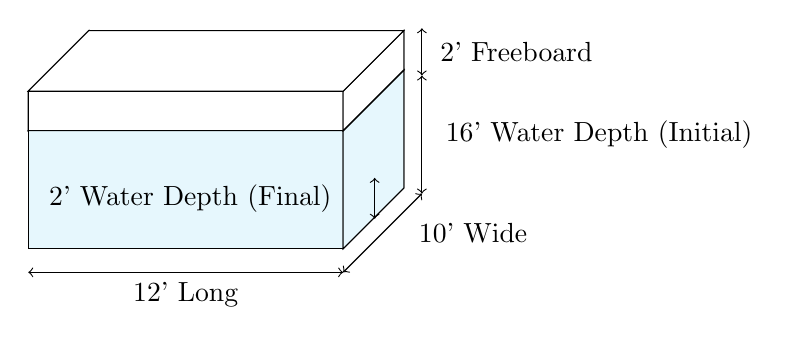
\begin{tikzpicture}

\pgfmathsetmacro{\cubexx}{4}
\pgfmathsetmacro{\cubeyy}{1.5}
\pgfmathsetmacro{\cubezz}{2}
\pgfmathsetmacro{\cubex}{4}
\pgfmathsetmacro{\cubey}{0.5}
\pgfmathsetmacro{\cubez}{2}
\pgfmathsetmacro{\cubexxx}{4}
\pgfmathsetmacro{\cubeyyy}{4}
\filldraw [fill=cyan!10!white, draw=black] (0,-\cubey,0) -- ++(-\cubexx,0,0) -- ++(0,-\cubeyy,0) -- ++(\cubexx,0,0) -- cycle ;
\filldraw [fill=cyan!0!white, draw=black] (0,-\cubey,0) -- ++(0,0,-\cubezz) -- ++(0,-\cubeyy,0) -- ++(0,0,\cubezz) -- cycle;
\filldraw [fill=cyan!10!white, draw=black] (0,-\cubey,0) -- ++(0,0,-\cubezz) -- ++(0,-\cubeyy,0) -- ++(0,0,\cubezz) -- cycle;
%\filldraw [fill=cyan!10!white, draw=black] (0,-\cubey,0) -- ++(-\cubexx,0,0) -- ++(0,0,-\cubezz) -- ++(\cubexx,0,0) -- cycle;
%%%\draw (0,-0.5,0) -- ++(-\cubex,0,0) -- ++(0,-\cubey,-\cubez) -- ++(\cubex,0,0) -- cycle;
\draw (-\cubex,0,0) -- ++(0,0,-\cubez) -- ++(0,-\cubey,0) -- ++(0,0,\cubez) -- cycle;
\draw (0,-\cubey,0) -- ++(-\cubex,0,0) -- ++(0,0,-\cubez) -- ++(\cubex,0,0) -- cycle;
\filldraw [fill=white, draw=black] (0,0,0) -- ++(-\cubex,0,0) -- ++(0,-\cubey,0) -- ++(\cubex,0,0) -- cycle ;
\filldraw [fill=white, draw=black] (0,0,0) -- ++(0,0,-\cubez) -- ++(0,-\cubey,0) -- ++(0,0,\cubez) -- cycle;
\filldraw [fill=white, draw=black] (0,0,0) -- ++(0,0,-\cubez) -- ++(0,-\cubey,0) -- ++(0,0,\cubez) -- cycle;
\filldraw [fill=white, draw=black] (0,0,0) -- ++(-\cubex,0,0) -- ++(0,0,-\cubez) -- ++(\cubex,0,0) -- cycle;

%\filldraw [fill=RoyalBlue!10!white, draw=black] (0,-1.5,0) -- ++(-\cubex,0,0) -- ++(0,-\cubey,0) -- ++(\cubex,0,0) -- cycle ;

%\filldraw [fill=RoyalBlue!10!white, draw=black] (0,-1.5,0) -- ++(0,0,-\cubez) -- ++(0,-\cubey,0) -- ++(0,0,\cubez) -- cycle;



%%\draw (0,-0.5,0) -- ++(-\cubex,0,0) -- ++(0,0,-\cubez) -- ++(\cubex,0,0) -- cycle;
%%\filldraw [fill=white, draw=black] (-\cubex,0,0) -- ++(0,0,-\cubez) -- ++(0,-\cubey,0) -- ++(0,0,\cubez) -- cycle;
%%\filldraw [fill=white, draw=black] (0,-\cubey,0) -- ++(-\cubex,0,0) -- ++(0,0,-\cubez) -- ++(\cubex,0,0) -- cycle ;

\draw [<->] (-4,-2.3) -- (0,-2.3) node [midway, below] {12' Long};
\draw [<->] (1,-1.3) -- (1,.2) node [midway, midway] {\hspace{4.5cm}16' Water Depth (Initial)};
\draw [<->] (0.4,-1.62) -- (0.4,-1.1) node [midway, midway] {\hspace{-4.8cm} 2' Water Depth (Final)};
\draw [<->] (1,.8) -- (1,.2) node [midway, midway] {\hspace{2.4cm}2' Freeboard};
\draw [<->] (1,-1.3) -- (0,-2.3) node [midway, midway] {\hspace{2.3cm}10' Wide};
\end{tikzpicture}\\
Volume to be pumped=$12 \enspace ft*10 \enspace ft *(16-2)\enspace ft=1,680ft^3$\\
\vspace{0.3cm}
$\implies \dfrac{1,680\cancel{ft^3}*7.48\dfrac{\cancel{gal}}{\cancel{ft^3}}}{600\dfrac{\cancel{gal}}{min}}=\boxed{21min}$
\end{enumerate}

\chapterimage{TitleIII.png} % Chapter heading image

\chapter{Wastewater Constituents and Analysis}
% \begin{enumerate}[1.]
% 	\definecolor{shadecolor}{RGB}{200, 200, 240}

% 	%%%%%%%%%%%
% 	% LEVEL 2 %
% 	%%%%%%%%%%%

% 	\begin{snugshade*}
% 		\item \noindent\textsc{Wastewater Constituents}%$$$$$$$$$$$$$$$$$$$$%
% 	\end{snugshade*}
% 	Solids, organic matter, nutrients, pathogens and oil \& grease are the main target constituents of wastewater treatment operations.
% 	\begin{enumerate}[A.]%___________%
% 			\definecolor{shadecolor}{RGB}{225, 235, 235}

				%%%%%%%%%%%
				% LEVEL 3 %
				%%%%%%%%%%%
		% \begin{snugshade*}
		% 	\item \noindent\textsc{Organic Matter}%###############################%
		% \end{snugshade*}
		
		\section{Organics}\index{Organics}		
		\begin{itemize}
			\item The main reason for treating domestic wastewater is to remove the organic matter.  
			\item Organics are substances containing carbon, hydrogen and oxygen, and some of which may be combined with nitrogen, sulfur or phosphorous.
			\item About 50 percent of the solids present in wastewater are organic.  This fraction is generally of animal or vegetable life, dead animal matter, plant tissue or organisms, and also include synthetic organic compounds.
			\item The principal organic compounds present in domestic wastewater are proteins, carbohydrates and fats together with the products of their decomposition.
			\item Organics are subject to decay or decomposition through the activity of bacteria and other living organisms.  \hl{Since the organic fraction can be driven off at high temperatures, they are also called \textbf{volatile solids}}.\
			\item \emph{Organics in wastewater is typically quantified in terms of oxygen required to oxidize the carbon based material present} in wastewater using the following methods:\\
\subsection{Biochemical Oxygen Demand (BOD)}\index{Biochemical Oxygen Demand (BOD)}

			  %     \begin{enumerate}[i.]
			  %     	\definecolor{shadecolor}{RGB}{220,220,220}
					% %%%%%%%%%%%
					% % LEVEL 4 %
					% %%%%%%%%%%%
			  %     	\begin{snugshade*}
			  %     		\item \noindent\textsc{Biochemical Oxygen Demand (BOD)}%@@@@@@@@@@@@@@@@@@%
			  %     	\end{snugshade*}					
			      	\begin{itemize}
			      		\item The BOD of wastewater is measured in terms of oxygen required for the microorganisms to consume the organic material present.
			      		\item BOD is typically measured as BOD$_5$ which is the oxygen demand of the wastewater measured after 5 days of the initiation of the test.
			      		\item The test involves incubating a known dilution of wastewater in a 300 ml bottle for 5 days at 20\si{\degree}C.  The dissolved oxygen (DO) content at the start and end of the incubation period is used for calculating the BOD.
			      		\item For the test to be considered valid, the following criteria need to be met: 1) DO consumption during the test must be at least 2 mg/l, 2) DO remaining at the end of the test must be at least 1 mg/l, and 3) DO consumed in blank should be 0.2 mg/l or less
			      		      			
			      		\item BOD is a parameter to measure the strength of wastewater and the measurement of the wastewater treatment plant or treatment process influent and effluent BOD is standard practice to measure its performance.  Typical domestic wastewater BOD is about 200-250 mg/l.
			      		\item The oxygen consumed by the microorganisms during the BOD test is primarily for: 1) Oxidizing the carbonaceous material (cBOD – carbonaceous BOD), and 2) Oxidizing nitrogenous constituents such as ammonia (nBOD – nitrogenous BOD).
			      		\item Thus, BOD (Total) = cBOD + nBOD.  The cBOD and nBOD is measured by adding certain chemical inhibitors which will inhibit the bacteria responsible for consuming the nitrogenous matter, thus measuring only the cBOD as part of the BOD test.
			      		\item Since not all of the organics is metabolized in the 5 days of the regular BOD test, certain wastewater discharge permits require reporting of the ultimate BOD value (BOD$_U$)\\
			      	\end{itemize}

			    \subsection{Chemical Oxygen Demand (COD)}\index{Chemical Oxygen Demand (COD)}
			      	% \begin{snugshade*}
			      	% 	\item \noindent\textsc{Chemical Oxygen Demand (COD)}%@@@@@@@@@@@@@@@@@@%
			      	% \end{snugshade*}		  
			      	\begin{itemize}
			      		\item The COD test involves using chemical oxidizers to measure the oxygen demand of the wastewater.
			      		\item As the chemical oxidizers will oxidize other constituents present, including inorganic matter, the COD value of wastewater will be higher than the BOD.  
			      		\item The COD test can be conducted rather quickly than the 5 day BOD test, it is an effective method to quantify the wastewater strength and process efficiencies and allow operators to make timely process adjustments.
			      	\end{itemize}

			    \subsection{Total Organic Carbon (TOC)}
			      	% \begin{snugshade*}
			      	% 	\item \noindent\textsc{Total Organic Carbon (TOC):}\\%@@@@@@@@@@@@@@@@@@%
			      	% \end{snugshade*}
			      	The TOC method utilizes laboratory analytical instruments which directly measure the organic carbon content by quantifying the amount of carbon dioxide produced from the complete combustion of the organics present.
			      % \end{enumerate}
		\end{itemize}
		
		
		
			\hl{Note: BOD measures the amount of oxygen required by the microorganisms present to consume the organic material while COD measures the chemical oxidation required to oxidize all chemicals including organics present in wastewater.  BOD value of typical domestic sewage is about 200 - 250 mg/l while the COD value ranges from 300 - 450 mg/l.  Typical BOD:COD ratio ranges from 0.5-0.8.}\\


\section{Solids}\index{Solids}
% 		\pagebreak
% 				\begin{snugshade*}
% 			\item \noindent\textsc{Solids}
% 		\end{snugshade*}	
		Like BOD, wastewater solids is another critical parameter for establishing the wastewater strength and determining treatment process efficiencies. 
		\begin{itemize}
			\item The \texthl{solids can be classified as suspended or dissolved} based upon its ability to pass through a standardized filter paper.
			\item When the wastewater is filtered:
			      \begin{itemize}
			      	\item the residual solids remaining on the filter paper after drying in an oven at 103\si{\degree}C is the \hl{suspended solids} portion, and 
			      	\item the solids remaining after drying the filtrate are the \hl{dissolved solids}.
			      \end{itemize}
			\item Suspended solids include larger floating particles and consist of sand, grit, clay, fecal matter, paper, pieces of wood, particles of food and garbage, and similar materials.
			\item Suspended solids can be categorized based upon its settling characteristics as:
			      \begin{itemize}
			      	\item \hl{Settleable}
			      	\item \hl{Non-settleable}
			      	      \begin{itemize}
			      	      	\item \hl{Colloidial}-small, charged (typically negative) particles which do not settle easily.  Some of the colloidial particles are small enough to pass through the filter paper used for filtering the suspended solids
			      	      	\item \hl{Floatable}-example oil and grease and small plastics
			      	      \end{itemize}
			      \end{itemize}
			\item Dissolved solids in wastewater include organics.  However, the major elements of dissolved solids are inorganic ions such as Ca$^{+2}$, Mg$^{+2}$, Cl$^-$, SO$_4$ $^{-2}$ , HCO$_3$ $^-$, Fe$^{+2}$, PO$_4$ $^{-3}$, NO$_3$ $^-$.  These ions are part of the dissolved salts such as sodium chloride (NaCl), calcium bicarbonate (Ca(HCO$_3$)$_2$), magnesium phosphate (Mg$_3$PO$_4$) and others which are normally present in water and wastewater. 
			      \begin{itemize}
			      	\item Conductivity or electrical conductance (EC) measurement is typically conducted as the wastewater enters the plant as \hl{conductivity provides an indirect and simple measure of the amount of dissolved solids present.}  
			      	\item Conductivity or electrical conductance (EC) is a measure the amount of electrical current that can be conducted by a solution.  
			      	\item The conductance of electricity in a solution is due to the presence of dissolved inorganic ions 
			      	\item The higher the concentration of these ions, the higher is the conductivity. 
			      	\item \underline{Conductivity is measured in the units of mhos/cm or Siemens/cm.}  (Note:  mhos is the reverse of ohm which is a measure of resistance).
			      	\item Typical wastewater conductivities range from 50 to 1500 S/cm
			      \end{itemize}
			\item Both suspended and dissolved solids can be either \hl{volatile (organic)} or \hl{fixed (inorganic)}.
			\item \hl{Total Solids is thus a sum of TSS and dissolved solids or volatile and fixed solids.}
			      \begin{itemize}
			      	\item The volatile solids are typically of plant or animal origin .
			      	\item The fixed solids include sand, gravel and silt as well as the dissolved salts.
			      \end{itemize}
			      \begin{minipage}{0.5\textwidth}
			      	\item The volatile or fixed fractions are quantified by incinerating the solids in a muffler furnace at 550\si{\degree} which removes only the volatile solids leaving only the fixed solids behind.
			      	\item In terms of the size of the solids, the distribution is approximately thirty percent suspended and about seventy percent dissolved solids - which includes the colloidal particles which have passed through the filter paper.\\ 
			      	\item As primary treatment process involve settling of solids, establishing the settleable portion of the suspended solids is important.\\  
			      	\item \hl{The settleable solids are quantified using an Imhoff cone and are reported in ml/L}.  Imhoff cone is a 1 liter, clear cone shaped container, with volume graduations (ml) at the bottom.
			      						
			      \end{minipage}	
			      \begin{minipage}{0.5\textwidth}
			      	\begin{center}
			      		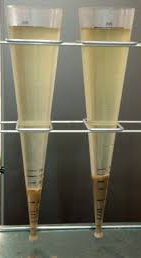
\includegraphics[scale=0.7]{ImhoffCone}\\
			      		Imhoff Cone\\
			      		\textit{Note the ml markings at the bottom of the cone}
			      		
			      		
			      	\end{center}
		      \end{minipage}
%			      \end{minipage}
			      	\item One factor which affects settleability is the conveyance time of the sewage to the treatment plant. 			
			      	\item The settleable component of the suspended solids will decrease as the sewage becomes more septic due to longer conveyance times.
			\item Influent and effluent total suspended solids are measured to establish the overall treatment and individual process efficiencies.  
			\item Volatile solids measurements before and after biological processes such as secondary treatment and digestion provide information on the process efficiency.\\
		\end{itemize}


	\subsection{Procedures for Solids Analysis}\index{Procedures for Solids Analysis}
% 		\begin{enumerate}%$$$$$$$$$$$$$$$$$$$$%
% 			\definecolor{shadecolor}{RGB}{220, 220, 220}
% 			\begin{snugshade*}
% 				\item \noindent\textsc{Procedures for Solids Analysis}
% 			\end{snugshade*}		
	\subsubsection{Determining wastewater suspended solids - Total(TSS) and Volatile(VSS) concentrations}\index{Determining wastewater suspended solids - Total(TSS) and Volatile(VSS) concentrations}			
			% \begin{enumerate}[a.]
			% 	\definecolor{shadecolor}{RGB}{110, 192, 221}
			% 	\begin{snugshade*}
			% 		\item \noindent\textsc{Determining wastewater suspended solids - Total(TSS) and Volatile(VSS) concentrations:}
			% 	\end{snugshade*}
				 
				%\hl{How total suspended solids concentration is established for a wastewater sample:}
				\begin{itemize}
					\item A known volume of wastewater sample is filtered through a pre-weighed filter paper
					\item The suspended solids will be retained by the filter
					\item The water with the dissolved solids will pass through the filter
					\item The filter paper with the filter solids is rinsed with distilled water to remove 
					\item The filter paper with the solids is dried in the oven and then weighed
					\item The difference between the weight of the dried filter paper with the solids and the pre-weighed filter paper, measured in mg, will be the suspended solids in: mg per the original quantity of wastewater sample taken.  This value can be converted to give the suspended solids content in mg/l
					\item A filter paper with the dried solids is incinerated in a muffler furnace
					\item The difference in the weight of the solids, before and after incineration is the fixed solids
					\item The difference between the weight of the solids before incineration and the fixed solids is the volatile solids
				\end{itemize}
				
	\subsubsection{Determining wastewater and sludge total solids (TS) and volatile solids (VS) concentrations}\index{Determining wastewater and sludge total solids (TS) and volatile solids (VS) concentrations}				
				
				% \begin{snugshade*}
				% 	\item \noindent\textsc{Determining wastewater and sludge total solids (TS) and volatile solids (VS) concentrations:}
				% \end{snugshade*}
				\begin{itemize}
					\item A certain quantity of wastewater (by volume) or sludge (by weight) is taken in a pre-weighed dish and weighed.  Note:  the sample is not filtered.
					\item The dish with the sample is dried in an oven
					\item The difference in the weight of the pre-weighed dish from that of the dish with the dried sample is the total solids
					\item The dried solids are incinerated in a muffler furnace
					\item The difference in the weight of the solids, before and after incineration is the fixed solids
					\item The difference between the fixed solids and the total solids is the volatile solids
					\item Total solids of a sludge sample is reported as a \% of the sludge weight.  A 7\% sludge has 7 lbs of solids for every 100 lbs of sludge.
				\end{itemize}
				
							
				
				
					\hl{For sludge samples, volatile solids is typically reported as the volatile solids fraction in \% of the total solids content of the sludge.  For example, if a 8\% sludge (i.e sludge which has 8\% TS or 80,000mg/l solids), is reported to have 70\% volatile, it means that 70\% of the total solids - 0.7*8\%=5.6\% or 56,000mg/l is the sludge volatile solids content.  \emph{70\% volatile does not meet the sludge has 700,000mg/l volatile solids}}\\
				
% 			\end{enumerate}
	\subsection{Summary of Wastewater Solids}\index{Summary of Wastewater Solids}		
% 			\begin{snugshade*}
% 				\item \noindent\textsc{Summary of Wastewater Solids}
% 			\end{snugshade*}
			\begin{itemize}
				\item Solids in wastewater can be categorized as dissolved or suspended
				      \begin{itemize}
				      	\item Suspended solids can be further categorized as settleable or unsettleable
				      \end{itemize}
				\item Solids can also be categorized as organic (aka: volatile) or inorganic (aka: fixed)
				\item Colloidial particles are small sized particles some of which pass through the filter and accounted as part of dissolved solids
				\item TSS - Total Suspended Solids are the solids that are captured on the filter paper upon filtration of the wastewater sample.  
				\item Wastewater samples typically analyzed for TSS include:  plant, primary and secondary processes - influent and effluent.  TSS is reported in mg/l
				\item TS - Total Solids are solids content of sludge.  TS of sludge is established by drying a preweighed quantity of sludge in an oven and is typically reported as \% solids - which is how many parts (by weight) of solids per 100 parts (by weight) of sludge.
				\item Volatile solids are solids that are removed when the solids are incinerated at 550C.  The solids that remain after incineration are fixed or non-volatile or inorganic solids.
			\end{itemize}
	\subsubsection{Wastewater Solids Content}\index{Wastewater Solids Content}			
% 			\begin{snugshade*}
% 				\item \noindent\textsc{Typical influent wastewater contains:}
% 			\end{snugshade*}
			\begin{itemize}
				\item Less than 0.1\% total solids.  Total solids concentration in typical wastewater is about 750mg/l
				\item The total solids are 50\% organic (volatile) and 50\% inorganic (fixed)
				\item Of the total solids, dissolved solids constitute about 70\% of the solids and the remaining 30\% solids are suspended solids
				\item 40\% of the dissolved solids are volatile the remaining 60\% are fixed
				\item 70\% of the suspended solids are volatile and the remaining 30\% are fixed
			\end{itemize}
			% \clearpage\thispagestyle{empty}
			\begin{figure}[!htbp]
			\vspace{2cm}
				\begin{center}
					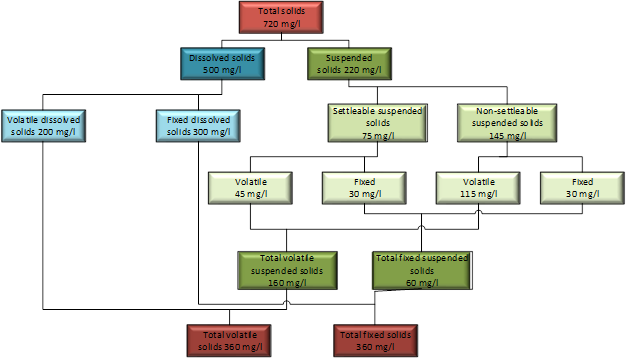
\includegraphics[scale=0.8]{WastewaterSolids}\\
					\caption{Typical Wastewater Solids Concentrations}
				\end{center}
				\end{figure}
% % 			\end{enumerate}
				
\section{Nutrients}\index{Nutrients}	
% 			\begin{snugshade*}
% 				\item \noindent\textsc{Nutrients}
% 			\end{snugshade*}	
			\begin{itemize}
				\item Plant nutrients - nitrogen and phosphorous, present in wastewater effluent discharge, promote growth of plant and algal matter in the receiving waters causing destruction of the normal aquatic life mainly due to oxygen depletion - eutrophication.
				      
				\item Because of the potential impacts of the presence of these nutrients in wastewater effluent on the receiving waters,  limits on the levels of these nutrients is typically stipulated in the treatment plant's wastewater discharge permit.
				      
				\item Typically, conventional secondary treatment processes are designed primarily remove the organics from the wastewater.  Secondary treatment process designed to additionally remove nutrients is deemed as tertiary or advanced treatment is termed as Biological Nutrient Removal (BNR).
			\end{itemize}
	\subsection{Nitrogen}\index{Nitrogen}				
% 			\begin{enumerate}%@@@@@@@@@@@@@@@@@@%
% 				\definecolor{shadecolor}{RGB}{220,220,220}
% 				\begin{snugshade*}
% 					\item \noindent\textsc{Nitrogen}%@@@@@@@@@@@@@@@@@@%
% 				\end{snugshade*}

	\subsubsection{Forms of nitrogen}\index{Forms of nitrogen}	
% 				\begin{itemize}
% 					\item Forms of nitrogen:\\
					      \begin{itemize}
					      	\item About 60\% of nitrogen in wastewater is present as ammonia nitrogen (about 60\%).  The ammonium nitrogen is present either in the form of ammonia (NH$_3$ ) or as ammonium (NH$_4^+$ ) ion.   These two forms can rapidly change from one to the other depending on pH and temperature.  Under low pH (acidic) or neutral conditions – pH less than or equal to 7, ammonia exists mostly as ammonium.  Ammonia becomes the dominant form as the pH increases to 8 and beyond.
					      	\item The other dominant form of nitrogen, about 40\% of the total nitrogen is as organic nitrogen
					      	\item Nitrogen measured as Total Kjeldahl Nitrogen (TKN) which is the sum of the organic nitrogen and the ammonia nitrogen concentrations.  Total inorganic nitrogen is the total concentration of ammonia nitrogen, NO3-, and NO2-.   Table provides the concentrations and forms of nitrogen in wastewater.
					      \end{itemize}
					      \setlength{\arrayrulewidth}{0.7mm}
					      \setlength{\tabcolsep}{8 pt}
					      \renewcommand{\arraystretch}{0.8}
					      \begin{center}
					      \begin{figure}[!htbp]
					      	\noindent \begin{tabular}[!htbp]{ |p{6cm}|p{2.0cm}|p{2.5cm}|p{2.cm}|}
					      	\hline
					      	\multicolumn{4}{|c|}{\textbf{Forms of Nitrogen in Wastewater}} \\
					      	\hline
					      	%\thead{A Head} & \thead{A Second \\ Head} & \thead{A Third \\ Head} \\
					      	%\hline%
					      	
					      	\hspace{1.8 cm}Forms of Nitrogen & \hspace{0.25 cm} Formula & \hspace{.4 cm} Found in & \hspace{.4 cm} Typical \newline \hspace{.2 cm}Concentration\\
					      	\hline
					      	\small Ammonia/Ammonium & \small NH$_3$/NH$_4^{\enspace +}$ &  \small Influent wastewater & 30-50 mg/l\\
					      	
					      	Total Kjeldahl Nitrogen \newline  \small (Ammonia/Ammonium + Organic Nitrogen) &  \small TKN &  \small Wastewater \newline  \small effluent  & 30-60 mg/l \\
					      	
					      	\small Total Inorganic Nitrogen \newline  \small (Ammonia/Ammonium + Nitrite + Nitrate) & \small TIN &  \small  Wastewater \newline  \small effluent  & 1-40 mg/l \\
					      	
					      	\small Nitrate  & $NO_3^{\enspace -}$ &  \small Nitrified effluent &  \small 1-35 mg/l \\
					      	
					      	\small Nitrate  &  $NO_2^{\enspace -}$ &  \small Partially nitrified effluent &  \small 0.1-2 mg/l \\
					      	
					      	\hline
					      	\end{tabular}
					      	\caption{Forms of Nitrogen}
					      	\end{figure}
					      \end{center}
					      
		\subsection{Phosphorous}\index{Phosphorous}			
		\subsubsection{Forms of phosphorous}\index{Forms of phosphorous}
					      \begin{itemize}
					      	\item The principal forms are organically bound phosphorus, polyphosphates, and orthophosphates.
					      	\item Organically bound phosphorus originates from body and food waste and, upon biological decomposition of these solids, is converted to orthophosphates. 
					      	\item Polyphosphates originate from synthetic detergents and are hydrolyzed to orthophosphates. Thus, the principal form of phosphorus in wastewater is assumed to be orthophosphates, although the other forms may exist. Orthophosphates consist of the negative ions PO$_4$$^{3-}$, HPO$_4$$^{2-}$, and H$_2$PO$_4$ $^-$.  These may form chemical combinations with cations (positively charged ions).
					      \end{itemize}

\section{Oil and Grease}\index{Oil and Grease}	
			Fats, oil and grease in wastewater originate from homes, food establishments and industries.
			\begin{itemize}
				\item Oil and grease content of wastewater is established in the laboratory by extracting it with a solvent - \textit{n}-hexane.  The concentration of oil and grease is reported in mg/l and typical oil and grease content of wastewater ranges from 80 - 120 mg/l
				\item Presence of excessive oils and grease could potentially impact the secondary treatment process
				\item Oils and grease are removed as floatables in primary treatment and sent with the sludge to the digesters
			\end{itemize}
		



\section{Wastewater Parameters}\index{Wastewater Parameters}			
		Laboratory and field tests are conducted to measure parameters which are critical for monitoring and controlling treatment.  The following are the key parameters that are measured.	
			
\subsection{pH}\index{pH}	
			\hl{pH is a measure of the hydrogen ion (H$^+$) content or the acidity or basicity of a solution.}  pH impacts the chemical and micribiological elements of wastewater treatment processes and thus pH measurement and control is critical.
			\begin{itemize}
				\item Pure water dissociates into equal concentration of hydrogen ions and hydroxide ions:\\ 
				      $H_2O \rightarrow H^+ + OH^-$.
				\item The H$^+$ are responsible for acidic properties and the OH$^-$ ions for the basic properties.  
				\item pH is the inverse of H$^+$ concentration; pH increases when the concentration of H$^+$ decreases relative to the concentration of OH-. 
				\item pH scale ranges from 0 – 14. When the concentration of both H$^+$ and OH$^-$ are equal, as in pure water, it is considered neutral and its pH is 7.0.  \item If the pH of a sample solution is below 7.0, the sample is termed acidic and is alkaline or basic if its pH is above 7.0. 
				\item Each change of 1 pH unit represents a 10 fold change in concentration.  For example, a sample with a pH of 2.0 is 1000 times more acidic than a sample with a pH of 5.0. 
				\item pH is measured by an electrode that is sensitive only to H$^+$ or using a pH strip which is essentially an adsorbent paper which is pre-impregnated with chemicals which change color under different H$^+$ concentrations.
				\item Most organisms involved in biological wastewater treatment processes do well within a a narrow range of pH near neutral (pH of 7).			
			\end{itemize}
			
\subsection{Oxidation Reduction Potential (ORP)}\index{Oxidation Reduction Potential (ORP)}			
			ORP is a measure of the potential of a wastewater to allow for microbiological oxidation and reduction reactions.\\
			An example of wastewater treatment process where microbiological oxidation involved include the activated sludge process.  Whereas, anaerobic digestion is a microbiological reduction based process.
			\begin{itemize}
				\item ORP value is measured in millivolts (mV), using an electrochemical probe
				\item The measured ORP value provides an indication of the potential of oxidation and reduction reactions in that sample.
				\item A higher positive ORP is indicative of oxidation potential of the wastewater whereas a negative ORP value indicates potential for a reduction reaction to occur.
				\item ORP measurements are used for controlling treatment processes including nitrification, odor control and disinfection.  For example, in the disinfection process utilizing chlorine (bleach), ORP measurements provides the strength of the oxidation potential of chlorine present in the wastewater being disinfected.  This measurement is used for precisely controlling the chlorine dosing.  The proper chlorine control results in optimizing chlorine dosing which reduces potential toxicity issues and dechlorination costs.
			\end{itemize}
			Typical ORP applications include the following processes and process elements
			
			
			\setlength{\arrayrulewidth}{0.3mm}
			\setlength{\tabcolsep}{8 pt}
			\renewcommand{\arraystretch}{0.8}
			\begin{center}
				\begin{tabular}{ |p{9.5cm}|p{4.0cm}|}
					\hline
					\multicolumn{2}{|c|}{\textbf{Typical Wastewater Process ORPs}} \\
					\hline
					
					\hline
					\small Collections	Sulfide formation                                & \small -50 to -250 mV  \\
					\small Influent wastewater                                          & \small - 200 mV        \\
					\small Activated sludge	cBOD degradation with free molecular oxygen & \small +50 to +250 mV  \\
					\small Biological phosphorous removal                               & \small +25 to +250 mV  \\
					\small Denitrification                                              & \small +50 to -50 mV   \\
					\small Anaerobic Digestion: Acid formation (Acidogenesis)           & \small -100 to -225 mV \\
					\small Anaerobic Digestion: Methane production (Methanogenesis)     & \small -75 to -400 mV  \\
					\hline
				\end{tabular}
				
			\end{center}
			
\subsection{Alkalinity}\index{Alkalinity}	
			\begin{itemize}
				\item \hl{Alkalinity is the ability of a water to neutralize acids.}  
				\item During certain wastewater treatment processes including anaerobic digestion, acids are generated as a result of microbiological activity.  The bacteria and other biological entities which play an active role in wastewater treatment are most effective at a neutral to slightly alkaline pH of 7 to 8.  In order to maintain these optimal pH conditions for biological activity there must be sufficient alkalinity present in the wastewater to neutralize acids generated by the active biomass.
				\item This ability to maintain the proper pH in the wastewater as it undergoes treatment is the reason why alkalinity is so important to the wastewater industry.
				\item The alkalinity is due to the presence of acid neutralizing bases in the water including the hydroxyl (OH$^-$), carbonate (CO$_3$$^-$) and bicarbonate (HCO$_3$$^-$)  ions.  These ions are of mineral origin and are also formed from carbon dioxide which comes from the atmosphere and from the microbial decomposition of organic material.  The resistance to pH change of the water will continue until all the alkalinity contributing ions are neutralized.  
				\item The pH of a water serves as a guide to the types of alkalinity present in the water but is unrelated to the alkalinity content of a water.  Important Note:  Alkalinity is a measure of the ability to neutralize acids whereas a solution is termed alkaline (or basic) if its pH greater than 7. 
				\item Alkalinity is expressed as milligrams per liter of CaCO$_3$
			\end{itemize}
			
\subsection{Dissolved Oxygen}\index{Dissolved Oxygen}	
			\begin{itemize}
				\item Dissolved oxygen (DO) is the concentration of oxygen dissolved in the wastewater sample and is typically measured in the field using a DO probe.  A titration based Winkler Test is used in the laboratory
				\item The \hl{presence of oxygen indicates an aerobic environment} where dissolved, free oxygen is available for aerobic microorganisms to live, BOD removal in the activated sludge process occurs as a result of the activity of aerobic bacteria.  The absence of DO indicates that the environment or condition is either anoxic or anaerobic.  
				\item \hl{In an anoxic environment, free oxygen is not present, but oxygen is available from its combined  forms - nitrate (NO$_3$ $^-$) and sulfate (SO$_4$ $^-$)} for the the consumption of microorganisms.  Example of an anoxic process is denitrification.  In denitrification, the anoxic bacteria in the presence of food (cBOD) consume the combined oxygen in nitrates (NO$_3$ $^-$ ) and convert it to nitrogen gas.
				\item \hl{The complete absence of oxygen including free and combined oxygen is an anaerobic environment.}
				\item Microorganisms are termed as obligate aerobes if they cannot survive without free oxygen.  Facultative aerobes are microorganisms which can survive in both aerobic and anaerobic environments.  
			\end{itemize}
			
\subsection{Microbiological testing and monitoring}\index{Microbiological testing and monitoring}	
			
			Microbiological testing and monitoring is conducted as part of the wastewater treatment for two main reasons:
			\begin{enumerate}[1.]
				\item Heterotrohic (organisms that consume organic material) microbes are responsible for the biological wastewater treatment processes - secondary treatment process, digestion and nutrient removal; and
				\item Pathogens - agents that cause disease are present in wastewater effluent.
			\end{enumerate}

\begin{itemize}
				
				\item Microbiological testing related to monitoring and troubleshooting biological wastewater treatment\\
				
				Microbes involved in biological wastewater treatment processes include:\\
				\begin{itemize}
					\item Fungi - Filamentous fungi occasionally bloom in activated sludge processes due to low pH or nutrient deficiency and cause problems with the settleability.
					\item Protozoa - Protozoas play a important role in the secondary treatment process.  Common protozoas in the activated sludge process include:
					      \begin{itemize}
					      	\item Amoeba
					      	\item Flagellate
					      	\item Cilliate
					      \end{itemize}
					\item Rotifers
					\item Nematodes
					\item Bacteria - Bacteria is the predominant microorganism responsible for the biological wastewater water treatment.  
				\end{itemize}
				\begin{itemize}
					\item The effectiveness of the biological wastewater treatment processes is primarily due to the presence of a microbial ecosystem with a right balance of populations of different microbial species.
					\item Methods used for monitoring the microbial composition include direct monitoring using a light microscope to see which and how many of the different microbial species are present - typically used for activated sludge process.
					\item Indirect method includes monitoring other parameters such as pH and alkalinity which are influenced by microbiological activity.
					\item The microbial monitoring ensures process stability and helps identify potential process upset conditions caused by changes to the microbial population due to other external factors - toxicty, organic loading, temperature etc.
				\end{itemize}

\item Microbiological testing related to monitoring and controlling pathogens in treated wastewater effluent\\

	
				Pathogens in wastewater belong to the following groups:
				\begin{itemize}
					\item Bacteria:  Although, bacteria is present in large numbers in feces, pathogenic or bacteria are present only because of an infection and this pathogenic bacteria can potentially spread the infection to other healthy individuals.  Disease spread by pathogenic bacteria include diarrhea, cholera and typhoid among many others.
					      
					\item Viruses: A large number of viruses may infect humans and are present in feces.  These include enteroviruses (including polioviruses), hepatitis A virus, reoviruses and diarrhea-causing viruses (especially rotavirus).
					      
					\item Protozoa:  Many species of protozoa can infect humans and cause diarrhoea and dysentery. Girardia which casues diarrheal illness is an example of a protozoan pathogen
					      
					\item Helminths:  These are parasitic worms that can infect humans and are transmitted to others through its eggs or larval forms
					      
				\end{itemize}
				
				\begin{itemize}
					\item As one of the main reasons for treating wastewater is to protect public health, microbiological/pathogen testing of the wastewater effluent and the surface water impacted by the wastewater discharge is conducted to meet the requirements of a wastewater discharge permit, to monitor the pathogen impact of treated wastewater discharge and assess the level of contamination of a public body of water.
					\item The bacteriological tests involves detection and quantification of one or more of the following bacteria:  total coliforms, fecal coliforms, E. Coli, and Enterococcus.  
					      \begin{itemize}
					      	\item The main reason why these bacteria such as coliforms and enterococcus are used \hl{as it is not practical to detect and quantify all pathogens associated with wastewater.}  
					      	\item These selected bacteria originate from feces and indicate fecal contamination and thus serve as an indicator organisms for pathogens of wastewater origin.  
					      	\item Also, they are abundant, potentially less harmful, and easy to detect.  E. coli has been shown to be a better predictor of the potential for impacts to human health and therefore many newer wastewater discharge permits require E. Coli testing in lieu of fecal coliform testing requirements.
					      \end{itemize}
					\item The microbiological test sample is always collected as a grab in a clean, sterile borosilicate glass or plastic bottle containing sodium thiosulfate. 
					      \begin{itemize}
					      	\item Sodium thiosulfate is added to remove residual chlorine which will kill coliforms during transit. 
					      	\item If the sample is not preserved or maintained under proper conditions until the test is conducted in the laboratory, the test would provide erroneous results.
					      	\item Samples must be refrigerated if they cannot be analyzed within 1 hour of collection and must be handled with care to prevent contamination and adverse conditions such as prolonged exposure to direct sunlight.
					      	\item The maximum holding time for state or federal permit reporting purposes is 6 hours. 
					      \end{itemize} 
					\item As it is not possible to exactly quantify the number of bacteria present, a statistical based - \hl{Most Probable Number (MPN)} approach is utilized.  The methods for wastewater bacteriological tests include:  multiple-tube fermentation technique, membrane filtration and quanti-tray testing. 
				\end{itemize}
			\end{itemize}

\subsection{Specific Gravity}\index{Specific Gravity}				
			\begin{itemize}
				\item Specific gravity is a term to express the weight of a solution with respect to that of water
				\item Water weighs 1 kg/L or 8.34 lbs/gallon or 62.4 lbs/ft$^3$
				\item A solution with a specific gravity of 1.2 will weigh 1.2 times the same volume of water.  1 L of that solution will weigh ( 1.2 kg )/L  or  ( 1.2*8.34=10lbs )/gallon.
				\item Typically wastewater and the associated unthickened sludge, for all practical purposes is assumed to have a specific gravity of 1 - implying 8.34 lbs/gallon.
				\item Specific gravity is typically used for calculations related to chemicals used in wastewater treatment.
			\end{itemize}
			
\section{Wastewater Sampling}\index{Wastewater Sampling}
		\begin{itemize}
			\item Field or laboratory measurement of a certain parameter is critical in wastewater treatment operations to obtain information about wastewater characteristics in order to either characterize a wastewater stream, or to monitor a treatment process or for permit compliance.  
			\item A sample is a small part of the whole representing the whole.  Thus, a sample needs to be such that it truly represents the entire population – which in a wastewater operations could be either a wastewater stream, wastewater solids or a chemical used.
		\end{itemize}
		
\subsection{Sampling Methods}\index{Sampling Methods}
\subsubsection{Grab Samples}\index{Grab Samples}
				\begin{itemize}
					\item A grab sample is a sample collected at a specific spot at a site over a short period of time.  
					\item Grab sampling allows for instantaneous analysis of parameters such as pH, dissolved oxygen, chlorine residual, temperature and other parameters which change rapidly with time.
					\item A grab sample represents a snapshot of space and time of a process stream.
					\end{itemize}
\subsubsection{Composite Samples}\index{Composite Samples}
				\begin{itemize}
					\item A composite sample is a collection of discrete samples are combined over a certain period or space and therefore represent the average performance of a wastewater treatment plant or a process during the collection period.\\  
					\item Composite sampling can be either based on:
					      
					      1. constant time interval (time proportioned sampling)\\
					      2. constant wastewater volume interval (flow-proportioned sampling), and\\
					      3. treatment process space - includes samples taken at different depths\\
					      
					\item Composite samples are typically collected using automated samplers which can be programmed to collect samples at pre-established time intervals – for time proportional sampling.
					\item Time and space composite samples are collected by adding equal volumes of samples collected from different times or locations.  
					\item Flow proportional composite samples comprise of volume of each subsample based on flow.\\  
				\end{itemize}
				
			\begin{center}
				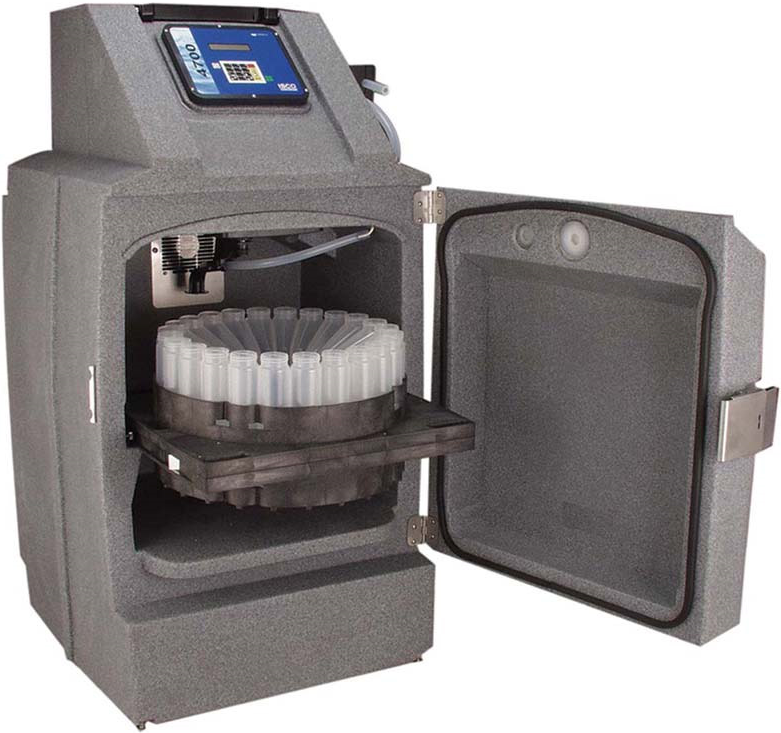
\includegraphics[scale=0.2]{Autosampler} \hspace{2cm} 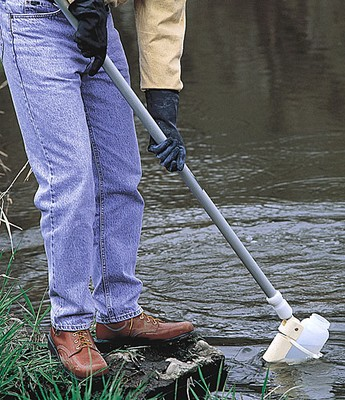
\includegraphics[scale=0.37]{Grabsampler}\\
			\end{center}
			\hspace{2.3cm} Automated Sampler \hspace{2.0cm} \parbox{\textwidth}{Grab Sampling Using a Long Handle Dipper}\\

\subsubsection{Sampling Precautions and Protocols}\index{Sampling Precautions and Protocols}
			\begin{itemize}
				\item Samples should represent the major portion of the process or the process stream and should be taken from places where the mixing is thorough, avoiding dead spots and areas of heavier or lighter loadings. 
				\item The collected sample is invariably exposed to conditions very different from the original source and is subject to change due to chemical and microbiological activity.  
				\item Thus, in order to ensure integrity of sample, sample preservation techniques specific to the analysis to be performed is needed.  
				      \begin{itemize}
				      	\item The preservation technique should not only allow for stabilizing the parameter to be analyzed, it should also not interfere with the analyses.  
				      	\item The common preservation techniques involve use of proper containers, temperature control, addition of chemical preservatives, and observance of the recommended maximum sample holding time.
				      \end{itemize}
			\end{itemize}

\section{Data Reporting}\index{Data Reporting}	
		\begin{itemize}
			\item Arithmetic mean is typically calculated for reporting data where multiple samples have been collected and analyzed for the same process stream at different times and for reporting average value over a certain time period – daily, monthly etc.\\ \item Arithmetic mean mathematically is calculated by adding all the result values and dividing by the total number of data points.\\
		\end{itemize}
		Mathematically the arithmetic mean is represented as:\\
		$$\bar{x}=\dfrac{\sum_{i=1}^{n} x^i}{n} = \dfrac{x_1+x_2+x_3...x_n}{n}$$
		For example:\\
		Arithmetic mean of the following set of data points:  200, 304, 250, 400 is calculated as:\\
		\vspace{10pt}
		Arithmetic Mean = $\dfrac{200 + 302 + 250 + 400}{4}= 288$\\
		\vspace{10pt}
		For data sets for analysis such as fecal coliform could include values which vary by several orders of magnitudes, using the arithmetic mean to report the average value is not appropriate as the lower or higher values would bias the calculated mean.\\
		\vspace{10pt}
		For example, consider a data set with values:  260, 300, 500, 5,000, 320 and 200.\\
		\vspace{10pt}
		The arithmetic mean = $\dfrac{260+300+500+5,000+320+200}{6} = 3,444$\\
		Here the 5000 value completely skews the arithmetic mean.
		
		Therefore, for such tests, the geometric mean calculation is used for reporting the average value.\\
		
		
		Mathematically a geometric mean is represented as:\\
		$$\Bigg(\prod_{i=a}^n\Bigg)^{\dfrac{1}{n}}=\sqrt[n]{a_1*a_2*a_3...a_n}$$
		 
		Calculation method:\\
		1.	Find the product of all the data points (analogous to first calculating the sum of all the data points when calculating the arithmetic mean)\\
		260*300*500*5,000*320*200 = 12,480,000,000,000,000\\
		2.	Raise the product to the inverse of the number of data points\\
		(*Using the power function of a scientific calculator)\\
		Here n (\# data points) = 6 $\implies$ geometric mean = $(12,480,000,000,000,000)^{\dfrac{1}{6}}   = 482$

\end{document}
%% This is an example of theorems.
%\part{Module 7}
%\input{WATR080 Module7.tex}
% \subsection{Several equations}\index{Theorems!Several Equations}
% This is a theorem consisting of several equations.

% \begin{theorem}[Name of the theorem]
% In $E=\mathbb{R}^n$ all norms are equivalent. It has the properties:
% \begin{align}
% & \big| ||\mathbf{x}|| - ||\mathbf{y}|| \big|\leq || \mathbf{x}- \mathbf{y}||\\
% &  ||\sum_{i=1}^n\mathbf{x}_i||\leq \sum_{i=1}^n||\mathbf{x}_i||\quad\text{where $n$ is a finite integer}
% \end{align}
% \end{theorem}

% \subsection{Single Line}\index{Theorems!Single Line}
% This is a theorem consisting of just one line.

% \begin{theorem}
% A set $\mathcal{D}(G)$ in dense in $L^2(G)$, $|\cdot|_0$. 
% \end{theorem}

% %------------------------------------------------

% \section{Definitions}\index{Definitions}

% This is an example of a definition. A definition could be mathematical or it could define a concept.

% \begin{definition}[Definition name]
% Given a vector space $E$, a norm on $E$ is an application, denoted $||\cdot||$, $E$ in $\mathbb{R}^+=[0,+\infty[$ such that:
% \begin{align}
% & ||\mathbf{x}||=0\ \Rightarrow\ \mathbf{x}=\mathbf{0}\\
% & ||\lambda \mathbf{x}||=|\lambda|\cdot ||\mathbf{x}||\\
% & ||\mathbf{x}+\mathbf{y}||\leq ||\mathbf{x}||+||\mathbf{y}||
% \end{align}
% \end{definition}

% %------------------------------------------------

% \section{Notations}\index{Notations}

% \begin{notation}
% Given an open subset $G$ of $\mathbb{R}^n$, the set of functions $\varphi$ are:
% \begin{enumerate}
% \item Bounded support $G$;
% \item Infinitely differentiable;
% \end{enumerate}
% a vector space is denoted by $\mathcal{D}(G)$. 
% \end{notation}

%------------------------------------------------

% \section{Remarks}\index{Remarks}

% This is an example of a remark.

% \begin{remark}
% The concepts presented here are now in conventional employment in mathematics. Vector spaces are taken over the field $\mathbb{K}=\mathbb{R}$, however, established properties are easily extended to $\mathbb{K}=\mathbb{C}$.
% \end{remark}

% %------------------------------------------------

% \section{Corollaries}\index{Corollaries}

% This is an example of a corollary.

% \begin{corollary}[Corollary name]
% The concepts presented here are now in conventional employment in mathematics. Vector spaces are taken over the field $\mathbb{K}=\mathbb{R}$, however, established properties are easily extended to $\mathbb{K}=\mathbb{C}$.
% \end{corollary}

%------------------------------------------------

% \section{Propositions}\index{Propositions}

% This is an example of propositions.

% \subsection{Several equations}\index{Propositions!Several Equations}

% \begin{proposition}[Proposition name]
% It has the properties:
% \begin{align}
% & \big| ||\mathbf{x}|| - ||\mathbf{y}|| \big|\leq || \mathbf{x}- \mathbf{y}||\\
% &  ||\sum_{i=1}^n\mathbf{x}_i||\leq \sum_{i=1}^n||\mathbf{x}_i||\quad\text{where $n$ is a finite integer}
% \end{align}
% \end{proposition}

% \subsection{Single Line}\index{Propositions!Single Line}

% \begin{proposition} 
% Let $f,g\in L^2(G)$; if $\forall \varphi\in\mathcal{D}(G)$, $(f,\varphi)_0=(g,\varphi)_0$ then $f = g$. 
% \end{proposition}

%------------------------------------------------

% \section{Examples}\index{Examples}

% This is an example of examples.

% \subsection{Equation and Text}\index{Examples!Equation and Text}

% \begin{example}
% Let $G=\{x\in\mathbb{R}^2:|x|<3\}$ and denoted by: $x^0=(1,1)$; consider the function:
% \begin{equation}
% f(x)=\left\{\begin{aligned} & \mathrm{e}^{|x|} & & \text{si $|x-x^0|\leq 1/2$}\\
% & 0 & & \text{si $|x-x^0|> 1/2$}\end{aligned}\right.
% \end{equation}
% The function $f$ has bounded support, we can take $A=\{x\in\mathbb{R}^2:|x-x^0|\leq 1/2+\epsilon\}$ for all $\epsilon\in\intoo{0}{5/2-\sqrt{2}}$.
% \end{example}

% \subsection{Paragraph of Text}\index{Examples!Paragraph of Text}

% \begin{example}[Example name]
% \lipsum[2]
% \end{example}

%------------------------------------------------

% \section{Exercises}\index{Exercises}

% This is an example of an exercise.

% \begin{exercise}
% This is a good place to ask a question to test learning progress or further cement ideas into students' minds.
% \end{exercise}

%------------------------------------------------

% \section{Problems}\index{Problems}

% \begin{problem}
% What is the average airspeed velocity of an unladen swallow?
% \end{problem}

%------------------------------------------------

% \section{Vocabulary}\index{Vocabulary}

% Define a word to improve a students' vocabulary.

% \begin{vocabulary}[Word]
% Definition of word.
% \end{vocabulary}

%----------------------------------------------------------------------------------------
%	PART 3
%----------------------------------------------------------------------------------------

%\part{Analysis and Testing}

%----------------------------------------------------------------------------------------
%	CHAPTER 3
%----------------------------------------------------------------------------------------
%\input{WastewaterAnalysisandLaboratoryMethods.tex}
% \chapterimage{chapter_head_1.pdf} % Chapter heading image

% \chapter{Presenting Information}

% \section{Table}\index{Table}

% \begin{table}[h]
% \centering
% \begin{tabular}{l l l}
% \toprule
% \textbf{Treatments} & \textbf{Response 1} & \textbf{Response 2}\\
% \midrule
% Treatment 1 & 0.0003262 & 0.562 \\
% Treatment 2 & 0.0015681 & 0.910 \\
% Treatment 3 & 0.0009271 & 0.296 \\
% \bottomrule
% \end{tabular}
% \caption{Table caption}
% \label{tab:example} % Unique label used for referencing the table in-text
% %\addcontentsline{toc}{table}{Table \ref{tab:example}} % Uncomment to add the table to the table of contents
% \end{table}

% Referencing Table \ref{tab:example} in-text automatically.

% %------------------------------------------------

% \section{Figure}\index{Figure}

% \begin{figure}[h]
% \centering
\includegraphics[scale=0.5]{placeholder.jpg}
% \caption{Figure caption}
% \label{fig:placeholder} % Unique label used for referencing the figure in-text
% %\addcontentsline{toc}{figure}{Figure \ref{fig:placeholder}} % Uncomment to add the figure to the table of contents
% \end{figure}

% Referencing Figure \ref{fig:placeholder} in-text automatically.

%----------------------------------------------------------------------------------------
%%	BIBLIOGRAPHY
%%----------------------------------------------------------------------------------------
%
%\chapter*{Bibliography}
%\addcontentsline{toc}{chapter}{\textcolor{ocre}{Bibliography}} % Add a Bibliography heading to the table of contents
%
%%------------------------------------------------
%
%\section*{Articles}
%\addcontentsline{toc}{section}{Articles}
%\printbibliography[heading=bibempty,type=article]
%
%%------------------------------------------------
%
%\section*{Books}
%\addcontentsline{toc}{section}{Books}
%\printbibliography[heading=bibempty,type=book]
%
%%----------------------------------------------------------------------------------------
%%	INDEX
%%----------------------------------------------------------------------------------------
%
%\cleardoublepage % Make sure the index starts on an odd (right side) page
%\phantomsection
%\setlength{\columnsep}{0.75cm} % Space between the 2 columns of the index
%\addcontentsline{toc}{chapter}{\textcolor{ocre}{Index}} % Add an Index heading to the table of contents
%\printindex % Output the index

%----------------------------------------------------------------------------------------

\end{document}
